% This document describes how to use iiscthesis style
%%%%%%%%%%%%%%%%%%%%%%%%%%%%%%%%%%%%%%%%%%%%%%%%%%%%%%%%%%%%%%%%%%%%%%%%%%%
\documentclass[12pt,twosides]{iiscthes}
\pagestyle{bfheadings}
%\newcommand{\minp}{(\min,+)}


%\usepackage{times}
%\usepackage{helvet}
\usepackage{paralist}
\usepackage{latexsym}
\usepackage{url}
\usepackage[all]{xy}
\usepackage{graphicx}
\usepackage{etex}
\usepackage{amsmath}
\usepackage{amssymb}
\usepackage{comment}
\usepackage{enumitem}
\usepackage{xcolor}
\usepackage{xspace}
\usepackage{tikz}
\usepackage{pgfplots}
\usepackage{pgfplotstable}
\usepackage{pgf}
\usepackage{natbib}
\usepackage{algorithmic}
%\usepackage{algorithmicx}
%\usepackage{algorithm2e}
\usepackage{algorithm}
\usepackage{savesym}
\usepackage{gnuplotluatikz}
\usepackage{gnuplottex}
\savesymbol{AND}
\usepackage{xspace}
\usepackage{placeins}
\pgfplotsset{filter discard warning=false}
\usepgfplotslibrary{external} 
\tikzexternalize[optimize=false] 
%\usepackage{style/ssltr}
%\usepackage{style/macros}
\usetikzlibrary{intersections}
\usetikzlibrary{arrows,calc,fit,patterns,plotmarks,shapes.geometric,shapes.misc,shapes.symbols,   shapes.arrows,   shapes.callouts,   shapes.multipart,   shapes.gates.logic.US,   shapes.gates.logic.IEC,   er,   automata,   backgrounds,   chains,   topaths,   trees,   petri,   mindmap,   matrix,   calendar,   folding, fadings,   through,   positioning,   scopes,   decorations.fractals,   decorations.shapes,   decorations.text,   decorations.pathmorphing,   decorations.pathreplacing,   decorations.footprints,   decorations.markings, shadows,circuits}
\tikzstyle{decision}=[diamond,draw]
\tikzstyle{line}=[draw]
\tikzstyle{elli}=[draw,ellipse]
\tikzstyle{arrow} = [thick]
%\usepackage{subfig}
\newcommand{\mb}{\mbox{ }}
\newcommand{\one}{\mathbf{1}}
\newcommand{\nn}{\nonumber}
\newcommand{\minp}{(\min,+)}
\newcommand{\maxp}{(\max,+)}
\newcommand{\V}{\mathcal{V}}
\newcommand{\R}{\mathbf{R}}
\newcommand{\Rm}{\mathbf{R}_{\min}}
\newcommand{\Ls}{\mathcal{L}}
\newcommand{\ra}{\rightarrow}
\newcommand{\om}{\otimes}
\newcommand{\op}{\oplus}
\newcommand{\nd}{n\times d}
\newcommand{\RA}{\Rightarrow}
\newcommand{\LA}{\Leftarrow}
\newcommand{\E}{\mathbf{E}}
\newcommand{\T}{\mathcal{T}}
\newcommand{\B}{\mathcal{B}}
\newcommand{\F}{\mathcal{F}}
\newcommand{\C}{\mathcal{C}}
\newcommand{\M}{\mathcal{M}}
\newcommand{\N}{\mathcal{N}}
\newcommand{\et}{||\Gamma J^*-\hg J^*||_\infty}
\newcommand{\etmn}{||\Gamma J^*-\hg J^*||_{\mn}}
\newcommand{\ini}{\lceil \frac{n}{k}\rceil}
\newcommand{\I}{\mathcal{I}}
\newcommand{\mut}{\tilde{\mu}}
\newcommand{\mn}{\infty,1/\psi}
\newcommand{\tj}{\tilde{J}_c}
\newcommand{\hj}{\hat{J}_c}
\newcommand{\jd}{J'_c}
\newcommand{\bj}{\bar{J}}
\newcommand{\tv}{\tilde{V}}
\newcommand{\hv}{\hat{V}}

\newcommand{\tu}{\tilde{u}}
\newcommand{\hu}{\hat{u}}

\newcommand{\muh}{\hat{\mu}}
\newcommand{\mui}{{\mu}^i}

\newcommand{\br}{\bar{r}}
\newcommand{\hr}{\hat{r}_c}
\newcommand{\tr}{\tilde{r}_c}

\newcommand{\cf}{\mathcal{F}}







\newcommand{\tg}{\tilde{\Gamma}}



\newcommand{\conf}{\sqrt{\frac{2\ln t}{t_i}}}
%\newcommand{\tg}{\tilde{\Gamma}}
\newcommand{\hg}{\hat{\Gamma}}
\newcommand{\gd}{\Gamma'}
\newcommand{\vd}{V'}
%\newcommand{\qed}{\blacksquare}

\newcommand{\keywords}[1]{{\bf Keywords: } #1\par}
\newenvironment{proof}{{\bf Proof:} }{}
\newtheorem{theorem}{Theorem}
\newtheorem{lemma}[theorem]{Lemma}
\newtheorem{assumption}{Assumption}
\newtheorem{definition}[theorem]{Definition}
\newtheorem{proposition}[theorem]{Proposition}
\newtheorem{corollary}{Corollary}
\newtheorem{remark}{Remark}
\newtheorem{example}{Example}
\newtheorem{note}{Note}
\newcommand{\alert}[1]{\textcolor{red}{#1}} 



\def\v{\mathbf{v}}
\def\r{\mathbf{r}}
\def\p{\mathbf{p}}
\def\q{\mathbf{q}}
\def\R{\mathrm{R}}
\def\Re{\mathbb{R}}
\def\Z{\mathbb{Z}}
\def\P{\mathrm{P}}
\def\S{\mathcal{S}}
\def\A{\mathcal{A}}

\newcommand{\ith}[2][th]{$#2^{\text{#1}}$}

\newcounter{subequation}[equation]
\newcommand{\thesubequationonly}{\alph{subequation}}
\renewcommand{\thesubequation}{\text{\theequation(\thesubequationonly)}}
\newcommand{\subequationitem}{\refstepcounter{subequation}(\thesubequationonly)\thinspace}

\def\mathdisplay#1{%
  \ifmmode \@badmath
  \else
    $$\def\@currenvir{#1}%
    \let\dspbrk@context\z@
    \let\tag\tag@in@display \SK@equationtrue %\let\label\label@in@display
    \global\let\df@label\@empty \global\let\df@tag\@empty
    \global\tag@false
    \let\mathdisplay@push\mathdisplay@@push
    \let\mathdisplay@pop\mathdisplay@@pop
    \if@fleqn
      \edef\restore@hfuzz{\hfuzz\the\hfuzz\relax}%
      \hfuzz\maxdimen
      \setbox\z@\hbox to\displaywidth\bgroup
        \let\split@warning\relax \restore@hfuzz
        \everymath\@emptytoks \m@th $\displaystyle
    \fi
%   \fi
}

\newcommand{\algorithmicinput}{\textbf{Input:} }
\newcommand{\INPUT}{\item[\algorithmicinput]}
\newcommand{\algorithmicoutput}{\textbf{Output:} }
\newcommand{\OUTPUT}{\item[\algorithmicoutput]}
\newcounter{algostep}
\newcommand{\Step}[1][\STATE]{#1\textbf{\refstepcounter{algostep}\thealgostep}. }

\newenvironment{algoequation}{\refstepcounter{equation}$}{$\hfill (\theequation)}

\newenvironment{nonfloatalgorithm}[1]{\vspace{1ex}\hrule\vspace{0.5ex} \refstepcounter{algorithm}\textbf{Algorithm \thealgorithm}\hspace{1em} #1 \vspace{0.5ex}\hrule}{\hrule\vspace{1.5ex}\setcounter{algostep}{0}}

\newcounter{acalgorithm}

\newenvironment{nonfloatactorcriticalgorithm}[1]{\vspace{1ex}\hrule\vspace{0.5ex} \textbf{Actor-Critic Algorithm \refstepcounter{acalgorithm}\theacalgorithm}\hspace{1em} #1 \vspace{0.5ex}\hrule\addcontentsline{loa}{algorithm}{\protect\numberline{\theacalgorithm}{\ignorespaces #1}}}{\hrule\vspace{1.5ex}\setcounter{algostep}{0}}

% Put your macros here
%\newfont{\punkbx}{punkbx20}

\begin{document}
%%%%%%%%%%%%%%%%%%%%%%%%%%%%%%%%%%%%%%%%%%%%%%%%%%%%%%%%%%%%%%%%%%%%%%%%%%%
% The frontmatter environment for everything that comes with roman numbering
\begin{frontmatter}
%%%%%%%%%%%%%%%%%%%%%%%%%%%%%%%%%%%%%%%%%%%%%%%%%%%%%%%%%%%%%%%%%%%%%%%%%%%
%
% Everything is optional in the front matter.
%
%%%%%%%%%%%%%%%%%%%%%%%%%%%%%%%%%%%%%%%%%%%%%%%%%%%%%%%%%%%%%%%%%%%%%%
%                         THE TITLEPAGE                              %
%%%%%%%%%%%%%%%%%%%%%%%%%%%%%%%%%%%%%%%%%%%%%%%%%%%%%%%%%%%%%%%%%%%%%%
\title{Reinforcement Learning- Results in Approximate Dynamic Programming and Stochastic Approximation
	}
\author{Chandrashekar Lakshminarayanan}
% For all the parameters below, take default values
\submitdate{JUNE 2015}
\dept{Computer Science and Automation}
\enggfaculty
%\degreein{Computer Science and Engineering}
%\mscengg
%\me
\iisclogotrue % Default is false
% \figurespagefalse %default is true
\tablespagetrue %default is false
\maketitle
\makecontents
\vspace{10MM}
\noindent
\end{frontmatter}
%%%%%%%%%%%%%%%%%%%%%%%%%%%%%%%%%%%%%%%%%%%%%%%%%%%%%%%%%%%%%%%%%%%%%%%%%%%%%
%%%%%%%%%%%%%%%%%%%%%%%%%%%%%%%%%%%%%%%%%%%%%%%%%%%%%%%%%%%%%%%%%%%%%%%%%%%%%

\chapter{Introduction}
The framework of Markov Decision Process (MDP) is useful to model and study problems involving optimal sequential decision in a variety of dynamic systems. MDPs occur natrually in domains such as science, engineering and economics. Ideally, we are interested in computing the optimal strategy/policy i.e., the decision rule that yields the best response. However, in practice, it is computationally expensive to find the optimal policy and we have to resort to approximate methods that provide us with sub-optimal policies. Further, in many cases, the model of the MDP is not known explicitly and only \emph{noisy} samples are available. One way to handle the nosie is to \emph{learn} in an iterative manner by taking smaller steps towards the solution.\par
The aim of this thesis is to shed light on the following important questions.
\begin{enumerate}
\item Under what conditions can we quantify the performance of the sub-optimal policy computed by approximate methods?
\item Under what conditions can we show convergence and stability of iterative methods that learn from noisy samples?
\end{enumerate}
\section {Markov Decision Process}
We provide a rigourous treatment of MDPs in Chapter~\ref{mdp}. Informally, in the MDP framework, the planner/decision-maker needs to perform an action at each decision epoch. The action fetches an immediate reward and the system moves to the next state.\par
In each of the above examples the planner needs to come up with a good policy i.e., a decision rule that specifies how the planner needs to act in each and every state so as to obtain satisfactory rewards. \par
\textbf{The problems of \emph{Control} and \emph{Prediction}}\\
The problem of \emph{control} deals with computing good policies, following which the planner obtains a desirable response. Also, each policy is associated with a value function that specifies the value of any state under the policy. In most cases, in turns out that, in order to compute better policy, the planner also needs to solve the problem of \emph{prediction} i.e., the planner needs to compute the value function of a given policy. Thus problem of prediction and the problem of control are inter-related.\par
%\subsection{Examples}
Dynamic Programming (DP) is a general principle to solve MDPs, the core of which constitutes the \emph{Bellman} equation (BE). The Bellman equation relates the optimal policy and the optimal \emph{value function}, i.e., it relates the prediction and control problems of a given MDP. A host of analytical and iterative methods exists to solve the Bellman equation for MDPs. These methods are known as exact dynamic programming methods since they spell out the optimal policy and value function exactly.\par
The three important exact DP methods are 
\begin{itemize}
\item Value Iteration.
\item Policy Iteration.
\item Linear Programming.
\end{itemize}
%\subsection{Problems of Control and Prediction}
%\subsection{Curse of Dimensionality}
%\subsection{Lack of Model Information}

%\section{Approximate Dynamic Programming}

%\subsection{Various Approaches} Leading to value function based ADP methods.
%\subsection{Key Ingredients}
%\subsection{Performance Guarantees}
%\subsection{Open Questions}

%\section{Reinforcement Learning}

%\subsection{Stochastic Approximation}
%\subsection{Open Questions}

%\section{Contributions and Organization}
\section{Practical Issues}
MDPs arising in practical problems are faced with two important issues. First issue is due to the \emph{curse-of-dimensionality} (or simply the \emph{curse}), a term which signifies the fact that the number of states of the MDP grows exponentially in the number of dimensions. Thus it becomes difficult to solve the MDP employing exact DP methods due to the overhead involved in computing, storing and retrieving the exact value function and policy for each and every state.\par
The second issue is the lack of model information, wherein, the the model parameters of the MDP are not available explicitly. However, the the underlying system can be simulator or sample trajectories via direct interaction with the system. This scenario is known as the \emph{reinforcement learning} setting since the model parameters have to be \emph{learned} by using the feedback obtained via direct interaction with the environment.\par
A wide range of methods/algorithms exist in literature to address the issues of the curse and the lack of model information. In particular, the methods that tackle the curse are broadly termed as approximate dynamic programming methods and methods that handle the case of lack of model information are called reinforcement learning algorithms. 
\section{Approximate Dynamic Programming}
Approximate Dynamic Programming (ADP) methods, as the name suggests, combine the ideas of approximate computations and dynamic programming. In practice, ADP methods tackle the curse by approximating the value function and/or the policy. A popular approach adopted by ADP methods is to first compute an approximate value function and obtain a sub-optimal policy by substituting the approximate value function in the Bellman equation. Loosely speaking, any ADP method has two parts to it namely:
\begin{enumerate}
\item Approximation architecture.
\item Scheme to compute the \emph{best} function within the chosen approximation architecture.
\end{enumerate}
The requirements of an approximation architecture are compact representation, easy storage and computation of the approximate value function. In most cases, ADP methods draw upon ideas from exact DP methods to compute the \emph{best} function within a given approximation architecture.\par
\begin{comment}
\begin{enumerate}
\item Approximation architecture.
\item Scheme to compute the right function within the chosen approximation architecture.
\end{enumerate}
In most cases, ADP methods are obtained by combining exact DP methods with a given approximation architecture. A given ADP scheme can be said to belong to either of two approaches based on the way the prediction and the control problems are addressed. The two distinct approaches are:
\begin{enumerate}
\item The \emph{value function} based approach, wherein a direct approximation to the optimal value function is obtained and a \emph{greedy/sub-optimal} policy is computed by substituing the approximate value function in the Bellman equation.
\item The \emph{approximate policy iteration} based approach, wherein, the critic evaluates the current policy, i.e., computes an approximation of the value function of the current policy. The actor on the other hand, makes use of the approximate value function to imporve the current policy.
\end{enumerate}
\end{comment}
\textbf{Performance Metrics}\\
The performance of a given ADP method can be quantified by the following metrics namely
\begin{itemize}
\item Prediction Error, i.e., the difference between the exact value function and the approximate value function.
\item Control Error, i.e., the loss in performance due to the sub-optimal policy as compared to the optimal policy.
\end{itemize}
Here the sub-optimal policy is the one that is obtained by substituting the approximate value function in the Bellman equation.
It is a known result that if the prediction error is bounded in the $\max$-norm (or $L_\infty$-norm), the control error can be bounded as well. The necessacity of $L_\infty$-norm  arises due to the fact that the Bellman operator is only a contraction map in the $L_\infty$ norm.\par
An ADP method is said to address both the prediction and control problems if it can offer guaranteed performance levels measured in terms of the aforementioned metrics. Given an ADP method, it a major theoretical challenge to come up with an analytical expression to bound the aforementioned performance metrics and it is in particlar difficult to bound the control error in many ADP schemes.\par
\section{Linear Function Approximation}
The first step in any ADP method is the choice of approximation architecture. In particular, a compact way of representing an approximation for the value function is necessary in most cases. A paramtererized function class is an useful approximation architecture since every function can be specified by the parameter it is enough to store only the parameters. Computing the right function that best approximates the exact value function then boils down to computations involving only the parameters and the curse can be tackled by choosing the number of parameters to be much lesser than the number of states. The most widely used parameterized class is the linear function approximator (LFA). Under a LFA, each function is written as a linear combination of pre-selected \emph{basis} functions. The exact value function is then approximated by computing/learning the weights of the various basis functions in the linear combination.\par
The method used to compute the right weights of the linear combination affects the quality of the approximation. The projected Bellman equation and the approximate linear programming are two different ways of computing the weights. These two differing approaches have their advantages/disadvantages and provide interesting research problems.\par
\textbf{Projected Bellman Equation}\\
%Once the basis functions of the LFA have been fixed, the right candidate function from the LFA has to be picked as the approximate value function. 
A candidate for the approximate value function could be that function which is at the least distance from the exact value function. Minimizing the distance between the linear combination of basis functions and the exact value function is similar to the idea of conventional \emph{linear regression} wherein, the target function is \emph{projected} onto the linear sub-space spanned by the basis functions. However, the idea of linear regression cannot be applied in a straightforward manner to compute the approximate value function because the exact value function (which is the target function in this case) is not known.\par
The Projected Bellman Equation (PBE) combines the idea of linear least squares projection and the Bellman equation. The central idea underlying the PBE is to find a fixed point in the linear sub-space spanned by the basis functions. However, existence of such a fixed point can be ensured only under a restricted setting. In particular, the Bellam operator is \emph{non-linear} and is a contraction map in the $\max$-norm ($L_\infty$-norm). On the other hand, the linear least squares projection operator is non-expansive only in the $L_2$-norm. As a direct consequence of the mismatch in norms the PBE based methods suffer from the shortcoming mentioned as under.
\begin{enumerate}
\item While the prediction error can be bound only in the $L_2$-norm and hence the control error cannot be quantified.
\item There are simple MDPs for which the PBE based solution methods are known to produce a sequence of policies that oscillate within a set of bad policies. This phenomenon is called as \emph{policy-chattering}.\par
\end{enumerate}

\begin{comment}
Hence the Bellman operator cannot be combined as such with the least squares projection operator. Neverthless, this issue can be side stepped by considering the Bellman operator restricted to a given policy which can be shown to be a contraction map in a generalized $L_2$-norm. The Bellman operator restricted to a given policy can be combined with the linear least squares projection operator to find a fixed point. However, such a fixed point can approximate only the value function of the particular policy (with respect to which the Bellman operator has been restricted) and not the optimal value function. As a consequence, the PBE can only be used for approximate policy evaluation, i.e., it can be used to compute an approximation to the value function of a given policy. 
This means that the PBE based methods fall into the category of approximate policy iteration approach, i.e., the approximate policy evaluation should be followed by a policy improvement step. However, there is a `norm-mismatch' between the projection operator that minimizes the error in $L_2$-norm and the $\max/L_\infty$-norm required to guarantee policy improvement. As a result, the sub-optimal policy obtained from the approximate value function computed by the PBE is not guaranteed to be an improvement.\par
\end{comment}
\textbf{\underline{Problem~$1$: Projected Bellman Equation in the $\minp$ linear basis}}\\
\begin{comment}
The major disadvantage of the PBE based methods is that they do not address the control problem completely. In fact, there are simple MDPs for which the PBE based solution methods are known to produce a sequence of policies that oscillate within a set of bad policies. This phenomenon is called as \emph{policy-chattering} and is a direct consequence of the norm mismatch.\par
\end{comment}
It is known that \cite{BertB} the issue of norm-mismatch can be alleviated if the projection operator preserves \emph{monotonicity}, i.e., if given two functions with one of them greater (component-wise) that the other, then the same holds for their projections as well. It is also known that the projection operator arising in the $\minp$ linear algebra preserves this monotonicity property. The first part of the thesis deals with developing convergent ADP methods based on $\minp$ linear algebra. In particular, the monotonicity property helps in
\begin{itemize}
\item Building convergent value function based ADP methods. Since the optimal value function is approximated directly, the issue of policy-chattering is absent.
\item Providing performance guarantees for the greedy/sub-optimal policy. This is possible since there is no issue of `norm-mismatch'.
\end{itemize}
\textbf{Approximate Linear Programming}\\
The approximate linear programming (ALP) formulation is obtained by introducing linear function approximation in the linear programming formulation (LP) of the given MDP. In contrast to the PBE, the ALP does not rely on the linear least squares projection operator, but instead, computes the approximate value function by optimizing a linear objective over a set of linear inequality constraints. In particular, the ALP restricts its search to a space of linear functions that upper bound the optimal value function. The ALP is a value function method as it computes an approximation to the optimal value function. Since, the corresponding greedy policy can be derived in a straightforward manner, the ALP does not suffer from issues of policy-chattering. Further, the ALP also offers good performance guarantees for both the prediction as well as the control problems, and thus addresses both the problems.\par
A significant shortcoming of the ALP formulation is that the number of constraints is of the order of the state space. Most MDPs arising in practice have a large number of constraints and hence it is always not possible to solve the ALP with all the constraints. However, there are some special cases of factored MDPs with factored value function representations that enable elimination of variables to come up with a tractable number of constraints. A general approach is to handle the large number of constraints is constraint sampling, wherein a Reduced Linear Program (RLP) is formulated by sampling fewer number of constraints from the orginial constraints of the ALP. Though the RLP is known to perform well in experiments, the theoretical analysis is available only for a specific RLP formulated under idealized settings.\par
\textbf{\underline{Problem~$2$: Framework to analyse constraint reduction in ALP:}}\\
The second part of the thesis deals with developing a novel theoretical framework to analyse constraint reduction/approximation in the ALP. The framework is built around studying a Generalized Reduced Linear Program (GRLP) whose constraints are obtained as positive linear combinations of the original constraints of the ALP. The salient features of the framework are
\begin{enumerate}
\item The analysis is based on two novel contraction maps and the error bounds are provided in a modified $L_\infty$-norm. Both the prediction and control error are bounded, thus making the GRLP a complete ADP scheme.
\item Justification of linear function approximation of the Lagrange multipliers associated with the constraints of the ALP. This is a desirable outcome, since both the primal and dual variables have linear function approximation.
\end{enumerate}
\section{Reinforcement Learning}
Reinforcement Learning (RL) algorithms can be viewed as `on-line'/sample trajectory based solution methods for solving MDPs. In the case of MDPs with a large number of states, RL algorithms are obtained as on-line versions of ADP methods. In order to handle the noise in the sample trajectory RL algorithms make use of stochastic approximation (SA). Typically, RL algorithm employing stochastic approximation are iterative schemes which take a small \emph{step} towards the desired value at each iteration. By making the right choice of the \emph{step-size} schedule effect of noise can be nullified and convergence to the desired value can be guaranteed.\par
Actor-Critic algorithms form an important sub-class of RL algorithms, wherein, the critic is responsible for policy evalutaion and the actor is responsible for policy improvement. In order to tackle the curse, the actor-critic schemes parameterize the policy and the value function. In an actor-critic algorithm, the critic forms the inner-loop and the actor constitutes the outer-loop. This is due to the fact that the actor has to needs the critic to evaluate a given policy before the actor updates the policy parameters. This effect of having two seperate loops can instead by achieved in practice by adopting different \emph{step-size} schedules for the actor and the critic. Specifically, the step-sizes used by the actor updates have to be much smaller than those used in the critic updates.\par
Stochastic approximation schemes that use different step-size schedules for different sets of iterates are known as multi timescale stochastic approximation schemes. The conditions under which the iterates of a multi timescale SA schemes converge to the desired value have been studied in literature. One of the conditions required to ensure the convergence of the iterates of a multi timescale SA scheme is that the iterates need to be stable, i.e., they should be bounded. However, the conditions that \emph{imply} the stability of the iterates in a multi timescale SA scheme have not been understood.\\
\textbf{\underline{Problem~$3$: Stability Criterion for Two Timescale Stochastic Approximation Schemes:}}\\
The third part of the thesis deals with providing conditions under which the stability of iterates in a two timescale stochastic approximation scheme follows. Salient features of the contribution are as follows:
\begin{enumerate}
\item The analysis is based on the ODE approach to stochastic approximation.
\item Stability of iterates of important actor-critic algorithms follow for the result.
\end{enumerate}
\section{Contributions and Organization}

%!TEX root =  autocontgrlp.tex
\chapter{Markov Decision Processes (MDPs)}
In this section, we briefly discuss the basics of Markov Decision Processes (MDPs) (the reader is referred to \cite{BertB,Puter} for a detailed treatment).\\
An MDP is a $4$-tuple $\langle S,A,P,g\rangle$, where $S$ is the state space, $A$ is the action space, $P$ is the probability transition kernel and $g$ is the reward function. We consider MDPs with large but finite number of states. We also assume that the number of actions is finite.
Without the loss of generality, we set  $S=\{1,2,\ldots,n\}$  and the action set is given by $A=\{1,2,\ldots,d\}$. For simplicity, we assume that all actions are feasible in all states. The probability transition kernel $P$ specifies the probability $p_a(s,s')$ of transitioning from state $s$ to state $s'$ under the action $a$. We denote the reward obtained for performing action $a\in A$ in state $s\in S$ by $g_a(s)$.

By a policy, we mean a sequence $\pi=\{\pi_0,\ldots,\pi_n,\ldots\}$ of functions $\pi_i, i\geq 0$ that describe the manner in which an action is picked in a given state at time $i$. The most general class of policies is the class of \emph{history-dependent randomized policies} denoted by $\pi$ and is defined below.
\begin{definition}
Let $h_n=\{s_0,\ldots,s_n, \pi_0, \ldots, \pi_{n-1}\}$ denote the \emph{history}. A policy $\pi$ is said to be a \emph{history-dependent randomized} policy if $\pi_n,n\geq 0$ is such that for every $s\in S$, $\pi_n(s,\cdot|h_n)$ is a probability distribution over the set of actions.
\end{definition}
We denote the class of policies by $\Pi$. The infinite horizon discounted reward corresponding to state $s$ under a policy $\pi$ is denoted by $J_\pi(s)$ and is defined by
\begin{align}
J_\pi(s)\stackrel{\Delta}{=}\E[\sum_{n=0}^\infty \alpha^n g_{a_n}(s_n)|\pi],\nn
\end{align}
where $a_{n} \sim \pi_n(s,\cdot)$ and $\alpha \in (0,1)$ is a given discount factor.  Here $J_\pi(s)$ is known as the value of the state $s$ under the policy $\pi$, and the vector quantity $J_\pi\stackrel{\Delta}{=}(J_\pi(s))_{s\in S}\in R^n$ is called the value-function corresponding to the policy $\pi$. The optimal value function $J^*$ is defined as $J^*(s)\stackrel{def}{=}\underset{\pi \in \Pi}{\max} J_\pi(s)$.\par
A stationary deterministic policy (SDP) is one where $\pi_n\equiv u$ for all $n\geq 0$ for some $u\colon S \ra A$. By abuse of notation we denote the SDP by $u$ itself instead of $\pi$. In the setting that we consider, one can find an SDP that is optimal \cite{BertB,Puter}, i.e., there exists an SDP $u^*$ such that $J_{u^*}(s)=J^*(s),\forall s\in S$. In this paper, we restrict our focus to the class $U$ of SDPs and without loss of generality we assume that there exists a unique SDP $u^*$ that is optimal. Under a stationary policy $u$ (or $\pi$), the MDP is a Markov chain and we denote its probability transition kernel by $P_u=(p_{u(i)}(i,j),i,j=1,\ldots,n)$ (or $P_\pi=(p_{\pi(i)}(i,j),i,j=1,\ldots,n)$, where $p_{\pi(i)}(i,j)=\sum_{a\in A}\pi(i,a)p_a(i,j)$ and $\pi(i)=(\pi(i,a), a\in A)$).\par
Given an MDP, our aim is to find the optimal value function $J^*$ and the optimal policy SDP $u^*$. The optimal policy and value function obey the Bellman equation (BE): for all $ s \in S$,
\begin{subequations}\label{bell}
\begin{align}
\label{bellval}J^*(s)&=\max_{ a\in A}\big(g_a(s)+\alpha \sum_{s'}p_a(s,s')J^*(s')\big),\\
\label{bellpol}u^*(s)&=\arg\max_{ a\in A}\big(g_a(s)+\alpha \sum_{s'}p_a(s,s')J^*(s')\big).
\end{align}
\end{subequations}
If $J^*$ is computed first, then $u^*$ can be obtained by substituting $J^*$ in \eqref{bellpol}. The Bellman operator $T$ is defined using the model parameters of the MDP as follows:
\begin{definition}
The Bellman operator $T: \R^n \to \R^n$ is defined by 
\begin{align}
(TJ)(s)=\max_{a \in A}\big(g_a(s)+\alpha \sum_{s'} p_a(s,s')J(s')\big)\,, 
\end{align}
where $J\in \R^n$ and $J_s = J(s)$, $s\in S = \{1,\dots,n\}$.  
Similarly one can define the Bellman operator $T_u:\R^n \to \R^n$ restricted to an SDP $u$ as follows:
\begin{align}
(T_uJ)(s)=g_{u(s)}(s)+\alpha \sum_{s'} p_{u(s)}(s,s')J(s')\,.
\end{align}
\end{definition}
Given $J \in \R^n$, $TJ$ is the `one-step' greedy value function. It is also useful to define the notion of a one-step greedy policy as below:
\begin{definition}
A policy $\tilde{u}$ is said to be greedy with respect to $\tilde{J}$ if
\begin{align}\label{subpol}
\tilde{u}(s)=\underset{a \in A}{\arg\max}  \big(g_a(s)+\alpha\sum_{s'} p_a(s,s')\tilde{J}(s')\big)
\end{align}
\end{definition}
We also define the Bellman operator $H$ for action values  \cite{BertB}:
\begin{definition}\label{bellactval}
Let $H: \R^n \to \R^{nd}$ be defined as follows: For $J\in \R^n$,
\begin{align}
HJ&=\left[ {\begin{array}{c} H_1 J  \\ \vdots \\ H_d J\end{array}} \right]\in \R^{nd},\mbox{where}\nn\\
(H_a J)(s)&= g_a(s)+\alpha \sum_{s'}p_a(s,s') J(s'), \qquad s\in S, a\in A.
\end{align}
\end{definition}
 We now state without proof the important properties related to the Bellman operator. Though in these results, we make use of the Bellman operator $T$, the results also trivially hold for $T_u$ as well.
\subsection{Properties of $T$}
\begin{lemma}\label{maxnorm}
$T$ is a $\max$-norm contraction operator, i.e., given $J_1, J_2 \in \mathbf{R}^n$,
\begin{align}
||TJ_1-TJ_2||_\infty\leq \alpha ||J_1-J_2||_\infty.
\end{align}
\end{lemma}
\begin{corollary}\label{uniquesol}
$J^*$ is a unique fixed point of $T$, i.e., $J^*=TJ^*$.
\end{corollary}
The Bellman operator $T$ exhibits two more important properties presented in the following lemmas (see \cite{BertB} for proofs):
\begin{lemma}\label{monotone}
$T$ is a monotone map, i.e., given $J_1,J_2 \in \R^n$ such that $J_2\geq J_1$, we have $T J_2\geq T J_1$. Further, if $J\in \R^n$ is such that $J\geq TJ$, it follows that $J\geq J^*$.
\end{lemma}
\begin{lemma}\label{shift}
Given $J\in \R^n$, $t \in \R$ and $\mathbf{1} \in \R^n$, a vector with all entries $1$, we have
\begin{align}
T(J+t\mathbf{1})=TJ+\alpha t\mathbf{1}.
\end{align}
\end{lemma}
Note that Lemmas~\ref{maxnorm}-\ref{shift} also hold for the Bellman operator $H$ defined for the action values in Definition~\ref{bellactval}.\par
Solving an MDP involves handling two sub-problems namely the problem of \emph{control} and the problem of \emph{prediction}. The problem of \emph{control} deals with coming up with a good (and if possible the optimal) policy. Often, in order to solve the problem of \emph{control}, one needs to solve the problem of \emph{prediction}, which deals with computing the value function $J_u$ of the policy $u$. The fact that the two problems are related is reflected in the Bellman equation in \eqref{bell}, where $J^*$ from \eqref{bellval} is used in \eqref{bellpol} to obtain the optimal policy $u^*$. Thus, the Bellman equation is at the heart of the solution methods to MDPs. Any solution method to MDP is said to be complete only if it satisfactorily (with provable performance guarantees) addresses both the prediction and the control problems. \\
The basic solution methods namely value iteration, policy iteration and linear programming (LP) formulation \cite{BertB} solve both the control and prediction problems. Of the three basic methods, in this paper, we are interested in the LP formulation given by
\begin{align}\label{mdplp}
\begin{split}
\min_{J\in \R^n}\, &c^\top J\\
\text{s.t}\mb &J(s)\geq g_a(s)+\alpha\sum_{s'}p_a(s,s')J(s'), \qquad s\in S, a \in A,
\end{split}
\end{align}
where $c\in \R^n_+$ is any vector whose components are all non-negative. One can show that $J^*$ is the solution to the LP formulation \eqref{mdplp} \cite{BertB}. 
Also, of the three methods, value iteration and LP formulation are value function based methods, i.e., they compute $J^*$ directly and then $u^*$ is obtained by plugging $J^*$ in \eqref{bellpol}.\\
While the basic methods (i.e., VI, PI and LP) can be used to compute exact values $J^*$ and $u^*$ for MDPs with a small number of states, they are computationally expensive in the case of MDPs with a large number of states.\\

%\chapter{Value Function Based Approximate Dynamic Programming}
\section{Curse of Dimentionality}
\emph{Curse-of-Dimensionality} is a term used to denote the fact that the number of states grows exponentially in the number of state variables. Most MDPs arising in practical applications suffer from the curse, i.e., have large number of states and it is difficult to compute $J^*/J_u\in \R^n$ exactly in such scenarios. Approximate dynamic programming (ADP) \cite{lspi,lspe,ALP,wang2014approximate} methods compute an approximate value function $\tilde{J}$ instead of $J^*/J_u$. In order to tackle the curse, ADP methods resort to dimensionality reduction by parameterizing the value function and/or the policy. Value-function based ADP methods form an important subclass of ADP methods whose brief overview is given below.
\section{Value Function Based Approximate Dynamic Programming}
In the value-function based ADP schemes a parameterized family is chosen and the approximate value-function $\tilde{J}$ is picked from the chosen parameterized class.
Once the approximate value function $\tilde{J}$ is computed, a sub-optimal policy $\tilde{u}$ can be obtained as the one-step greedy policy with respect to $\tilde{J}$ by making use of \eqref{subpol}.
The following lemma characterizes the degree of sub-optimality of the greedy policy $\tilde{u}$.
\begin{lemma}\label{subopt}
Let $\tilde{J}$ be the approximate value function and $\tilde{u}$ be as in \eqref{subpol}, then 
\begin{align}
||J^*-J_{\tilde{u}}||_\infty \leq \frac{2}{1-\alpha}||J^*-\tilde{J}||_\infty.
\end{align}
\end{lemma}
\begin{proof}
We know that
\begin{align}
\label{top} (T_{\tilde{u}}) \tilde{J}(s) 	&= g(s)+\alpha \sum_{s'} p_{\tilde{u}(s)} (s,s') \tilde{J}(s'),\\
\label{bot} J_{\tilde{u}}(s)		&=g(s)+\alpha \sum_{s'} p_{\tilde{u}(s)}(s,s')J_{\tilde{u}}(s').
\end{align}
Hence we can write by subtracting \eqref{top} from \eqref{bot} 
\begin{align}
J_{\tilde{u}}-\tilde{J}&=T_{\tilde{u}}\tilde{J}-\tilde{J} +\alpha P_{\tilde{u}}(J_{\tilde{u}}-\tilde{J}),\mb\text{or},\nn\\
J_{\tilde{u}}-\tilde{J}&=(I-\alpha P_{\tilde{u}})^{-1}(T_{\tilde{u}}\tilde{J}-\tilde{J}),\mb \text{hence}\nn\\
||J_{\tilde{u}}-\tilde{J}||_\infty&\leq \frac{1}{1-\alpha}||T_{\tilde{u}}\tilde{J}-\tilde{J}||_\infty.\nn
\end{align}
We know from \eqref{subpol} that $T_{\tilde{u}}\tilde{J}=T\tilde{J}$. Also from the fact that $J^*=TJ^*$ and the contraction property of $T$, we know $||T\tilde{J}-J^*||_\infty\leq \alpha ||\tilde{J}-J^*||_\infty$ and $||T_{\tilde{u}}\tilde{J}-\tilde{J}||_\infty\leq (1+\alpha)||\tilde{J}-J^*||_\infty$. Hence we have
\begin{align}
||J_{\tilde{u}}-J^*||_\infty&=||J_{\tilde{u}}-J^*+\tilde{J}-\tilde{J}||_\infty\nn\\
&\leq  ||J_{\tilde{u}}-\tilde{J}||_\infty+||\tilde{J}-J^*||_\infty\nn\\
&\leq \frac{1}{1-\alpha}||T_{\tilde{u}}\tilde{J}-\tilde{J}||_\infty +||J^*-\tilde{J}||_\infty\nn\\
&\leq \frac{1+\alpha}{1-\alpha}||J^*-\tilde{J}||_\infty +||J^*-\tilde{J}||_\infty\nn\\
&\leq \frac{2}{1-\alpha}||J^*-\tilde{J}||_\infty\nn.
\end{align}
\end{proof}
The quality of any ADP method depends on the approximation guarantees it offers for the quantities $||J^*-\tilde{J}||$ and $||J^*-J_{\tu}||$, where $||\cdot||$ is an appropriate norm. The term  $||J^*-\tilde{J}||$ denotes the error in prediction and $||J^*-J_{\tu}||$ denotes the loss in performance resulting from the sub-optimal policy $\tu$ with respect to the optimal policy $u^*$. Of the two error terms, $||J^*-J_{\tu}||$ is more important because ultimately we are interested in coming up with a useful policy. In the context of ADP methods, the control and prediction problems are said to be addressed when the error terms $||J^*-\tilde{J}||$ and $||J^*-J_{\tu}||$ are bounded by ``small'' constants.\\
\section{Linear Function Approximation}
The most widely used parameterized class to approximate the value-function is the linear function approximator (LFA). Under LFA, the value-function is approximated as $\tilde{J}=\Phi r^*$, with $\Phi=[\phi_1|\ldots|\phi_k]$ being an $n\times k$ feature matrix and $r^*$ is the parameter to be learnt.\\
%ADP methods vary in the way they compute the $\tj$ and $\tu$, and in what follows we present a short overview of some of the chief ADP methods while discussing their successes and shortcomings.
There are two important approaches to value function approximation. Both the approaches start out with a basic solution method and appropriately introduce function approximation in it. The two approaches are:
\begin{enumerate}
\item The Projected Bellman Equation (PBE) which combines the BE and the linear least squares projection operator to project high dimensional quantities onto the subspace of the LFA.
\item The approximate linear programming formulation which introduces the LFA in the linear programming formulation. 
\end{enumerate}



\chapter{Approximate Dynamic Programming in $\minp$ linear basis}
A host of ADP methods are based on the PBE and have been found to be useful in practice. The main application of the PBE is for approximate policy evaluation, i.e., to compute $\tilde{J}_u$, an approximation to the value function $J_u$ of policy $u$. Due to the mismatch in the norms, i.e, the linear least squares projection operator based on the $L_2$-norm and the $L_\infty$-norm of the Bellman operator $T$, one cannot use the PBE to obtain a direct approximation to $J^*$. Thus in order to solve the problem of control, $\tilde{J}_u$ is used to compute a one-step greedy policy. However, again due to the mismatch in the norms, i.e., $L_2$-norm of the linear least squares projection and the $L_\infty$ norm required for policy improvement (Lemma~\ref{subopt}), the one-step greedy policy need not necessarily be an improvement. This leads to a phenomenon called \emph{policy-chattering} \cite{dpchapter} where looping within of bad policies can occur. Further, such policy-chattering can be demonstrated in simple examples as well \cite{dpchapter}. Thus, though the approximate value function obtained by solving the PBE offers guarantees for prediction it does not offer any guarantees for the control problem, a significant shortcoming of the PBE based methods.\\
%However, an important shortcoming of the PBE based methods is the phenomenon called \emph{policy-chattering}. Such policy-chattering behavior can be demonstrated even on simple MDPs. 
%This happens due to the mismatch in the norms, i.e, the linear least squares projection operator based on the $L_2$-norm and the $L_\infty$ norm required for policy improvement (Lemma~\ref{subopt}). Thus, though the approximate value function obtained by the solving the PBE offers guarantees for prediction it does not offer any guarantees for the control problem, a significant shortcoming of the PBE based methods.\\
\section{Projected Bellman Equation}
A large class of ADP methods compute $r^*$ to be the solution to the projected Bellman equation (PBE) given below:
\begin{align}\label{pbelong}
\Phi r^*=\Phi (\Phi ^\top D_u\Phi)^{-1}\Phi^\top T_u\Phi r^*,
\end{align}
where $T_u$ is the Bellman operator corresponding to an SDP $u$ and $D_u$ is a $n\times n$ diagonal matrix whose diagonal entries are the stationary probabilities of the states under the SDP $u$. The PBE can be written in short as 
\begin{align}\label{pbe}
\Phi r^*=\Pi T_u \Phi r^*,
\end{align} where $\Pi=\Phi (\Phi ^\top D_u\Phi)^{-1}\Phi^\top$ is the projection operator. Notice that approximate value function $\tj=\Phi r^*$ obtained by solving the PBE \eqref{pbe} is an approximation only to $J_u$ and not $J^*$. This scenario is unavoidable because $T_u$ cannot be replaced by $T$ in \eqref{pbe}, since $\Pi T$ cannot be guaranteed to be a contraction map. As a result, an equation of the form $\Phi r=\Pi T\Phi r$ need not have a solution. Thus, the PBE can only be used for approximate policy evaluation, i.e., to compute $\tilde{J}_u\approx J_u$. Nevertheless, the solution to the PBE offers error bounds for the prediction problem and is given below:
\begin{align}\label{errbnd}
||J_u-\Phi r^*||_D \leq \frac{1}{\sqrt{1-\alpha^2}}||J_u-\Pi J_u||_D.
\end{align}
In order to address the problem of control, one resorts to approximate policy improvement (API) wherein a one-step look ahead policy is derived. The API scheme is given in Algorithm~\ref{appoliter}
\FloatBarrier 
\begin{algorithm}[H]
\caption{Approximate Policy Iteration (API)}
\begin{algorithmic}[1]
\STATE Start with any policy $u_0$
\FOR{$i=0,1,\ldots,n$} 
\STATE \label{appeval}Approximate policy evaluation $\tilde{J}_{i}= \Phi r^*_i$, where $\Phi r^*_i=\Pi T_{u_i}\Phi r^*_i$.
\STATE Improve policy $u_{i+1}(s)=\arg\max_a (g_a(s)+\alpha\sum_{s'}p_a(s,s')\tilde{J}_{i}(s'))$.
\ENDFOR
\RETURN $u_n$
\end{algorithmic}
\label{appoliter}
\end{algorithm}
The performance guarantee of API can be stated as follows:
\begin{lemma}\label{pgapi}
If at each step $i$ one can guarantee that $||\tilde{J}_i-J_{u_i}||_\infty\leq \delta$, then one can show that $\lim_{n\ra\infty}||J_{u_i}-J^*||\leq \frac{2\delta\alpha}{(1-\alpha)^2}$.
\end{lemma}
Note that the error bound required by Lemma~\ref{pgapi} is in the $L_\infty$ norm, whereas \eqref{errbnd} is only in the $L_2$ norm. So API cannot guarantee an approximate policy improvement at each step which is a shortcoming. Also, even-though each evaluation step (line~\ref{appeval} of Algorithm~\ref{appoliter}) converges, the sequence ${u_n}, n\geq0$ is not guaranteed to converge. This is known as policy $\emph{chattering}$. Thus the problem of $\emph{control}$ is only partially addressed by API, i.e, suffers in both convergence and performance guarantees. \\
In short, whilst the approximate value function obtained by the solving the PBE offers guarantees for prediction it does not offer any guarantees for the control problem. \\
In the next section, we discuss the approximate linear programming (ALP) formulation, the basic results and present prior results in literature as well as motivate the problem that we address in this paper. 



\section{$\minp$ linear functions}\label{semiring}
The $\Rm$ semiring is obtained by replacing multiplication ($\times$) by $+$, and addition ($+$) by $\min$.
\begin{definition}
\begin{align}
&\text{Addition:} &x \op y&= \min(x,y).\nn\\
&\text{Multiplication:} &x \om y&= x+y.\nn
\end{align}
\end{definition}
Henceforth we use, $(+, \times)$ and $(\op,\om)$ to respectively denote the conventional and $\Rm$ addition and multiplication respectively.
%We later justify the choice of $\minp$ linear basis for the discounted reward MDP setting.\\
A Semimodule over a semiring can be defined in a similar manner to vector spaces over fields. In particular we are interested in the semimodule $\mathcal{M}=\Rm^n$ (since $J^* \in \Rm^n$). Given $u, v \in \Rm^n$, and $\lambda \in \Rm$, we define addition and scalar multiplication as follows:
\begin{definition}
\begin{align}
(u\op v)(i)&=\min\{u(i),v(i)\}=u(i)\op v(i), \forall i=1,2,\ldots,n.\nn\\
(u\om \lambda)(i)&=u(i)\om \lambda=u(i)+\lambda, \forall i=1,2,\ldots,n.\nn
\end{align}
\end{definition}
Similarly one can define the $\R_{\max}$ semiring which has the operators $\max$ as addition and $+$ as multiplication.\\
\indent It is a well known fact that deterministic optimal control problems with cost/reward criterion are $\minp$/$\maxp$ linear (\cite{akian,Gaubert,mc2009,gaubert2011} ). However, it is straightforward to show that the Bellman operator $T$ (as well as $H$) in \eqref{bellops}  corresponding to infinite horizon discounted reward MDPs is neither $\minp$ linear nor $\maxp$ linear. Nevertheless, the motivation behind developing ADP methods based on $\minp$ LFAs is to explore them as an alternative to the conventional basis representation. \\
%Thus the aim is to understand the kind of convergence guarantees and error bounds that are possible in the $\minp$ LFAs.\\
Given a set of basis functions $\{\phi_i,i=1,\ldots,k\}$, we define the $\minp$ linear span to be $\mathcal{V}=\{v|v=\Phi\om r\stackrel{def}{=}\min(\phi_1+r(1),\ldots,\phi_k+r(k)), r \in \Rm^k\}$. Thus $\mathcal{V}$ is a subsemimodule. In the context of value function approximation, we would want to project quantities in $\Rm^n$ onto $\mathcal{V}$. The $\minp$ projection operator $\Pi_M$ works as follows (\cite{akian,cohen1996kernels,Gaubert}):
\begin{align}\label{smproj}
\Pi_M u=\min\{ v | {v \in \mathcal{V}}, v \geq u\}, \forall u \in \mathcal{M}.
\end{align}
We can write the PBE in the $\minp$ basis:
\begin{align}\label{projminpbasic}
v&=\Pi_M Tv, v\in \V\nn\\
\Phi \om r^*&=\min\{\Phi \om r^*\in \V|\Phi\om r^*\geq T \Phi \om r^*\}.
\end{align}
%Our choice of $\minp$ basis for reward problem is justified by the similarity in the structure of \eqref{projminpbasic} and the linear programming (LP) formulation of the infinite horizon discounted reward MDP.
Thus by making use of $\minp$ LFAs and the projection operator $\Pi_M$ we aim to find the minimum upper bound to $J^*$/$Q^*$. 
%A closely related ADP method is the approximate linear program (ALP), however, significantly differs from the formulation in \eqref{projminpbasic} in the algorithmic implementation and performance bounds, and a detailed discussion is out of scope of the paper.
\begin{comment}
\begin{align}\label{alp}
 &\mbox{ }\min ~c^\top \Phi r \\
      &\quad s.t\quad \Phi r(s)\geq g(s,a)+\alpha\sum_{s'}p_a(s,s')(\Phi r)(s'),\forall s \in S, a \in A\nn
\end{align}
\end{comment}

\section{Fenchel Dual and Projection on Subsemimodules}\label{fenchel}
In this section, we demonstrate the connections between the $\emph{Fenchel-Legendre}$ transform (FLT) and the $\minp$ projection defined in \eqref{smproj}. Given a function $f \colon \R^n \rightarrow \R$, its FLT is defined by $f^* \colon \R^n \ra \R$, with
\begin{align}\label{FT}
f^*(y)=\sup_{x \in \R^n}(y^\top x-f(x)), y \in \R^n.
\end{align}
If $f$ is convex, then it can be recovered as $f=f^{*^*}$, i.e.,
\begin{align}\label{FFT}
f(x)=f^{*^*}(x)=\sup_{y \in \R^n}(x^\top y-f^*(y)), x \in \R^n.
\end{align}
We can rewrite \eqref{FT} as below
\begin{align}\label{FTRR}
f^*(y)=\sup_{x \in \R^n}(f_y(x)-f(x)), y \in \R^n, \text{ where }f_y(x)=y^\top x.
\end{align}
Now instead of considering functions $f_y(x)$ indexed by $y \in \R^n$, we consider the sequence $\{\phi_j\}, j \in \mathcal{J}=\{1,2,\ldots,k\}, \phi_j \colon \R^n \ra \R$. Then \eqref{FTRR} can be modified as below:
\begin{align}\label{ST}
f^*(j)=\sup_{x \in \R^n}(\phi_j(x)-f(x)), j \in \mathcal{J}.
\end{align}
We call \eqref{ST}, the $\sup$-Transform or the $\max$-Transform. It is easy to check that $\phi_j(x)-f^*(j) <f(x), \forall x \in \R^n, j \in \mathcal{J}$. Since our index set in \eqref{ST} is finite (as opposed to $\R^n$ as in \eqref{FT} ), it is not necessary that the original function $f$ can be $\emph{reconstructed}$ from $f^*(j), j \in \mathcal{J}$. However, we can get an approximation $\tilde{f}$ as below:
\begin{align}\label{AST}
f(x)\approx\tilde{f}(x)=\sup_{j \in \mathcal{J}}(\phi_j(x)-f^*(j)).
\end{align}
In the light of \eqref{ST} and \eqref{AST}, the projection in \eqref{smproj} is nothing but the $\min$-Transform (as opposed to the $\max$-Transform \eqref{ST}). It is more clear if we rewrite \eqref{smproj} for the case when $\mathcal{V}=Span\{\phi_j|\phi_j \in \Rm^n, j=1,\ldots,k)$. Let $\Pi_M u=\Phi \om r^u$, then one can see that
\begin{align}
\Pi_M u&=\{\min\Phi\om r|\Phi \om r \geq u, r \in \Rm^k\}.\\
r^u(j)&= \min_{i =1,2,\ldots, n} (\phi_j(i)-u(i)), \forall j=1,2,\ldots,k.\label{mpproj}
\end{align}
Note the similarity between $r^u(j)$ in \eqref{mpproj} and $f^*(j)$ in \eqref{ST}.
Then the approximation/projection of $u$ onto $\mathcal{V}$ is given by $\tilde{u}=\Pi_M u=\Phi \om r^u$ with
\begin{align}\label{mplfa}
\Pi_M u(i)&=-\min_{j=1,\ldots,k}(\phi_j(i)+r^u(j))\nn\\
&=\phi_1(i) \om r^u(1)\op \ldots \op \phi_k(i) \om r^u(k).
\end{align}
Also, it is important to note that \eqref{ST} deals with projecting a function, while \eqref{smproj} deals with projecting the elements of $n$-dimensional semimodule. Nevertheless, the spirit of the projection is similar in both cases. Also, $\phi_j(i)+r^u_j -u(i)>0$, i.e., the $\min$-Transform approximates the given element $u$ by point-wise minimum of functions that upper bound $u$. We end this section with the following illustration.\\
\begin{example}
Let $f(x)=x^2$, and let $a=(a(j),j=1,\ldots,5)=(-0.8,-0.4,0,0.4,0.8)$, and $\phi_j(x)=2|x-a(j)|$. Then $\minp$ LFA of $f(x)$ via the $\min$-Transform using the $\{\phi_j(x),j=1,\ldots,5\}$ as the $\minp$ basis, is given in the Figure~\ref{minptrans}.
\end{example}
\begin{comment}
\begin{figure}\label{illust}
\begin{tikzpicture}[scale=1]
    \begin{axis}[
	xlabel=x,
        ylabel=f(x),
	]
    \addplot[smooth,black] plot file {mfiles/f.dat};
    \addplot[smooth,black] plot file {mfiles/fproj.dat};
    \addplot[dashed,black] plot file {mfiles/f1.dat};
    \addplot[dashed,black] plot file {mfiles/f2.dat};
    \addplot[dashed,black] plot file {mfiles/f3.dat};
    \addplot[dashed,black] plot file {mfiles/f4.dat};
    \addplot[dashed,black] plot file {mfiles/f5.dat};
%    \addplot[dashed,black] plot file {mfiles/f6.dat};
    \end{axis}
    \end{tikzpicture}
    \caption{$\minp$ LFA of $f(x)$}
    \label{minptrans}
\end{figure}
\end{comment}

\section{ Approximate $Q$ Iteration}\label{adpminp}
We now present an ADP scheme based on solving the PBE in $\minp$ basis to compute $\tilde{Q}(\approx Q^*)$. Our ADP scheme successfully addresses the two shortcomings of the ADP scheme in conventional basis. First, we establish contraction of the projected Bellman operator in the $L_\infty$ norm. This enables us to show that our recursion to compute $\tilde{Q}$ converges. We compute a greedy policy $\tilde{u}(s)=\max_a\tilde{Q}(s,a)$, and an approximate value function $\tilde{J}(s)=\max_a\tilde{Q}(s,a)$. Secondly, we also bound $||\tilde{Q}-Q^*||$ in the $\max$ norm which along with Lemma~\ref{subopt} gives a guarantee for $J_{\tilde{u}}$.\\
We are interested in solving the following PBE:%\footnote{We did not consider $\Phi \om r^*=\Pi_M T \Phi \om r^*$ since it approximates only $J^*$ and is superseded by \eqref{qpbe} which computes approximate $Q^*\approx\tilde{Q}$. Thus \eqref{qpbe} addresses both $\emph{prediction}$ and $\emph{control}$ problems. We wish to remind the reader of the discussion in section~\ref{appqlearn} on the issues with \eqref{qpbe} in conventional basis.}
\begin{align}\label{qpbe}
\Phi \om r^*=\Pi_M H \Phi \om r^*.
\end{align}
Since we want to approximate $Q^*$, $\Phi$ is an $nd\times k$ feature matrix, and $Q^*(s,a)\approx\tilde{Q}(s,a)=\phi^{(s-1)\times d+a}\om r^*$, where $\phi^i$ is the $i^{th}$ row of $\Phi$.
The Approximate $Q$ Iteration (AQI) algorithm is given by
\begin{align}\label{projqiter}
\Phi \om r_{n+1}=\Pi_M H \Phi \om r_n.
\end{align}
The following results help us to establish the fact that the projected Bellman operator $\Pi_M H\colon \Rm^{\nd}\ra \Rm^{\nd}$ is a contraction map in the $L_\infty$ norm. In the discussion that follows, $\mathbf{1} \in \R^\nd$ is a vector with all components equal to $1$.
\begin{lemma}\label{monotone}
For $Q_1, Q_2 \in \Rm^{\nd}$, such that $Q_1\geq Q_2$, we have $\Pi_M Q_1\geq \Pi_M Q_2$.
\end{lemma}
\begin{proof}
Follows from the definition of $\Pi_M$ in \eqref{smproj}.
\end{proof}
\begin{lemma}\label{shift}
Let $Q\in \Rm^{\nd}$, $V_1=\Pi_M Q$ be its projection onto $\V$. For $k\in \R$ the projection of $Q+k\mathbf{1}$ is $V_2=\Pi_M Q+k\mathbf{1}$.
\end{lemma}
\begin{proof}
We know that since $V_1\geq Q$, $V_1+k\mathbf{1}\geq Q+k\mathbf{1}$, and from the definition of the $\Pi_M$ in \eqref{smproj} $V_2\leq V_1+k\mathbf{1}$. Similarly $V_2-k\mathbf{1}\geq Q$, so $V_1\leq V_2-k\mathbf{1}$.
\end{proof}
\begin{theorem}\label{contra}
The projected Bellman operator $\Pi_M H$ is a contraction map in $L_\infty$ norm with modulus $\alpha$.
\end{theorem}
\begin{proof}
Let $Q_1,Q_2\in\Rm^{\nd}$, and $\epsilon\stackrel{def}{=}||Q_1-Q_2||_\infty$, then by Lemma~\ref{monotone} we have
\begin{align}
\Pi_M H Q_1- \Pi_M HQ_2&\leq \Pi_M H (Q_2+\epsilon\mathbf{1})-\Pi_M HQ_2\nn\\
				&=\Pi_M (H Q_2 +\alpha\epsilon\mathbf{1})-\Pi_M HQ_2\nn\\
				&=\alpha\epsilon\mathbf{1}.
\end{align}
Here the equality in second line is due to Lemma~\ref{shiftH}, and the final line follows from Lemma~\ref{shift}. Similarly $\Pi_M H Q_2- \Pi_M HQ_1\leq \alpha\epsilon\mathbf{1}$, so it follows that $||\Pi_M HQ_1-\Pi_MHQ_2||_\infty\leq \alpha ||Q_1-Q_2||_\infty$.
\end{proof}
\begin{corollary}\label{minpaviconv}
AQI in \eqref{projqiter} converges to a fixed point $r^*$ such that $\Phi \om r^*=\Pi_M H \Phi \om r^*$.
\end{corollary}

\section{Variational Approximate Q Iteration}\label{weakproj}
The projection operator $\Pi_M$ used in \eqref{projqiter} is exact. Let $v=\Pi_M u$, then for test vectors $w_i \in \Rm^n, i=1,\ldots,m$ it follows from the definition of $\Pi_M$ that
\begin{align}
w_i^\top v\geq w_i^\top u\nn
\end{align}
where the dot product $x^\top y=\min^n_{i=1}(x(i)+y(i))$. Let $W$ denote the $nd\times m$ test matrix whose columns are $w_i$. Now we shall define the approximate projection operator to be
\begin{align}\label{appproj}
\Pi^W_M u=\min\{v \in \mathcal{V}| W^\top v\geq W^\top u \}.
\end{align}
The superscript in $\Pi_M^W$ denotes the test matrix $W$. The Variational Approximate $Q$ Iteration (VAQI) is given by
\begin{align}\label{appprojqiter}
\Phi \om r_{n+1}= \Pi^W_M H\Phi \om r_n.
\end{align}
Lemmas~\ref{monotone},~\ref{shift}, and Theorem~\ref{contra} continue to hold if $\Pi_M$ is replaced with $\Pi^W_M$. Thus by Corollary~\ref{minpaviconv}, we know that \eqref{appprojqiter} converges to a unique fixed point $r^*_W$ such that $\Phi \om r^*_W=\Pi^W_M H\Phi \om r^*_W$.\vspace{-2pt}
\begin{comment}
\begin{theorem}\label{eboundapp}
Let $\tilde{r}$ be such that $\tilde{r}=\arg\min_r||Q^*-\Phi\om r||_\infty$. Let $r^*$ be the fixed point of the iterates in \eqref{appprojqiter}, then
\begin{align}
||Q^*-\Phi\om r^*||_\infty&\leq \frac{2}{1+\alpha}(||Q^*-\Phi\om \tilde{r}||_\infty\nn\\&\mbox{  }+||\Phi\om \tilde{r}-\Pi_M^W \Phi\om \tilde{r}||_\infty)
\end{align}
\end{theorem} 
\begin{proof}
Let $\epsilon=||Q^*-\Phi\om\tilde{r}||_\infty$, by contraction property of $H$ (Lemma~\ref{maxnorm}) we know that
\begin{align}
||HQ^*-H\Phi\om \tilde{r}||_\infty\leq \alpha \epsilon. \nn
\end{align}
So have $||\Phi\om\tilde{r}-H\Phi\om\tilde{r}||_\infty\leq (1+\alpha)\epsilon$. Then
\begin{align}
||\Phi\om\tilde{r}-\Pi^W_M H\Phi \om \tilde{r}||_\infty&=||\Phi\om\tilde{r}-\Pi^W_M \Phi \om \tilde{r}||_\infty\nn\\&+||\Pi^W_M\Phi\om\tilde{r}-\Pi^W_M H\Phi \om \tilde{r}||_\infty\nn
\end{align}
Now
\begin{align}
\Pi^W_M \Phi\om\tilde{r}-\Pi^W_M H\Phi \om \tilde{r}&\leq\Pi^W_M \Phi\om\tilde{r}\nn\\&-\Pi^W_M (\Phi \om \tilde{r}-(1+\alpha)\epsilon)\nn\\
&=(1+\alpha)\epsilon\nn
\end{align}
Similarly $\Pi^W_M H\Phi \om \tilde{r}-\Pi^W_M\Phi\om\tilde{r}\leq (1+\alpha)\epsilon$, and hence 
\begin{align}
||\Phi\om\tilde{r}-\Pi^W_M H\Phi \om \tilde{r}||_\infty\leq (1+\alpha)\epsilon+\beta,
\end{align}
where $\beta=||\Phi\om\tilde{r}-\Pi^W_M \Phi \om \tilde{r}||_\infty$. 
Now consider the iterative scheme in \eqref{appprojqiter} with $r_0=\tilde{r}$, and 
\begin{align}
||Q^*-\Phi\om r^*||_\infty&=||Q^*-\Phi\om r_0+\Phi\om r_0\nn\\&-\Phi\om r_1+\ldots-\Phi\om r^*||_\infty\nn\\
&\leq ||Q^*-\Phi\om r_0||_\infty+||\Phi\om r_0-\Phi\om r_1||_\infty\nn\\&+||\Phi\om r_1-\Phi\om r_2||_\infty+\ldots\nn\\
&\leq \epsilon+(1+\alpha)\epsilon+\beta+\alpha((1+\alpha)\epsilon+\beta)+\ldots\nn\\
&=\epsilon(\frac{1+\alpha}{1-\alpha}+1)+\frac{\beta}{1-\alpha}\nn\\
&=\frac{2\epsilon+\beta}{1-\alpha}\nn
\end{align}
\end{proof}
\begin{corollary}\label{polperf}
Let $r^*$ and $r^*_W$ be the fixed points of iterations \eqref{projqiter} and \eqref{appprojqiter} respectively, and let $\tilde{Q}=\Phi \om r^*$, $\tilde{Q}_W=\Phi \om r^*_W$. The greedy policies $\tilde{u}(s)=\arg\max_a \tilde{Q}(s,a)$ and $\tilde{u}_W(s)=\arg\max_a \tilde{Q}_W(s,a)$ obey
\begin{align}
||J_{\tilde{u}}-J^*||\leq \frac{2(2\epsilon)}{(1-\alpha)^2}, ||J_{\tilde{u}_W}-J^*||\leq \frac{2(2\epsilon+\beta)}{(1-\alpha)^2}
\end{align}
\end{corollary}
\begin{proof}
Follows from Theorem~\ref{eboundapp} and Lemma~\ref{subopt}, and the observation that the term $\beta$ is the error due to the usage of $\Pi^W_M$. Thus for solution to \eqref{qpbe} $\beta=0$.
\end{proof}
\end{comment}

\section{Error Analysis}
\begin{theorem}\label{eboundapp}
Let $\tilde{r}$ be such that $\tilde{r}=\arg\min_r||Q^*-\Phi\om r||_\infty$. Let $r^*_W$ be the fixed point of the iterates in \eqref{appprojqiter}, then
\begin{align}
||Q^*-\Phi\om r^*_W||_\infty&\leq \frac{2}{1+\alpha}(||Q^*-\Phi\om \tilde{r}||_\infty\nn\\&\mbox{  }+||\Phi\om \tilde{r}-\Pi_M^W \Phi\om \tilde{r}||_\infty).
\end{align}
\end{theorem} 
\begin{proof}
Let $\epsilon=||Q^*-\Phi\om\tilde{r}||_\infty$. By contraction property of $H$ (Lemma~\ref{maxnorm}) we know that
\begin{align}
||HQ^*-H\Phi\om \tilde{r}||_\infty\leq \alpha \epsilon. \nn
\end{align}
So we have $||\Phi\om\tilde{r}-H\Phi\om\tilde{r}||_\infty\leq (1+\alpha)\epsilon$. Then
\begin{align}
||\Phi\om\tilde{r}-\Pi^W_M H\Phi \om \tilde{r}||_\infty&=||\Phi\om\tilde{r}-\Pi^W_M \Phi \om \tilde{r}||_\infty\nn\\&+||\Pi^W_M\Phi\om\tilde{r}-\Pi^W_M H\Phi \om \tilde{r}||_\infty.\nn
\end{align}
\begin{align}
\text{Now},\mbox{ }\Pi^W_M \Phi\om\tilde{r}-\Pi^W_M H\Phi \om \tilde{r}&\leq\Pi^W_M \Phi\om\tilde{r}\nn\\&-\Pi^W_M (\Phi \om \tilde{r}-(1+\alpha)\epsilon)\nn\\
&=(1+\alpha)\epsilon.\nn
\end{align}
Similarly $\Pi^W_M H\Phi \om \tilde{r}-\Pi^W_M\Phi\om\tilde{r}\leq (1+\alpha)\epsilon$, and hence 
\begin{align}
||\Phi\om\tilde{r}-\Pi^W_M H\Phi \om \tilde{r}||_\infty\leq (1+\alpha)\epsilon+\beta,
\end{align}
where $\beta=||\Phi\om\tilde{r}-\Pi^W_M \Phi \om \tilde{r}||_\infty$. 
Now consider the iterative scheme in \eqref{appprojqiter} with $r_0=\tilde{r}$, and 
\begin{align}
||Q^*-\Phi\om r^*_W||_\infty&=||Q^*-\Phi\om r_0+\Phi\om r_0\nn\\&-\Phi\om r_1+\ldots-\Phi\om r^*_W||_\infty\nn\\
&\leq ||Q^*-\Phi\om r_0||_\infty+\nn\\&||\Phi\om r_0-\Phi\om r_1||_\infty\nn\\&+||\Phi\om r_1-\Phi\om r_2||_\infty+\ldots\nn\\
&\leq \epsilon+(1+\alpha)\epsilon+\beta+\alpha((1+\alpha)\epsilon+\beta)\nn\\
&+\ldots\nn\\
&=\epsilon(\frac{1+\alpha}{1-\alpha}+1)+\frac{\beta}{1-\alpha}\nn\\
&=\frac{2\epsilon+\beta}{1-\alpha}.\nn
\end{align}
\end{proof}
The error bound for AQI is obtained by letting $\beta=0$ in Theorem~\ref{eboundapp}.
\begin{corollary}\label{polperf}
Let $r^*$ and $r^*_W$ be the fixed points of iterations \eqref{projqiter} and \eqref{appprojqiter} respectively, and let $\tilde{Q}=\Phi \om r^*$, $\tilde{Q}_W=\Phi \om r^*_W$. The greedy policies $\tilde{u}(s)=\arg\max_a \tilde{Q}(s,a)$ and $\tilde{u}_W(s)=\arg\max_a \tilde{Q}_W(s,a)$ obey
\begin{align}
||J_{\tilde{u}}-J^*||\leq \frac{2(2\epsilon)}{(1-\alpha)^2}, ||J_{\tilde{u}_W}-J^*||\leq \frac{2(2\epsilon+\beta)}{(1-\alpha)^2},
\end{align}
where $\epsilon=\min_r||Q^*-\Phi\om r||_\infty$.
\end{corollary}
\begin{proof}
Follows from Theorem~\ref{eboundapp}, Lemma~\ref{subopt}, and the observation that the term $\beta$ is the error due to the usage of $\Pi^W_M$. Thus for solution to \eqref{qpbe}, $\beta=0$.
\end{proof}

\subsection{Experiment in Grid World}\label{exper}
We test our MPADP algorithm (Algorithm~\ref{algo1}) on a $10 \times 10$ grid world problem. There are a total of $100$ states, i.e., $S=\{1,2,\ldots,100\}$, and a grid position with the co-ordinate $(i,j)$ is encoded as the state $s=(i-1)\times 10+j$. The reward matrix is as given in Table~\ref{reward}, where each entry is an integer between $1$ and $10$. 
The grid world problem is used to model terrain exploration by autonomous decision making agents (robots).
In each grid position, the agent has $8$ actions corresponding to the $8$ possible directions. In the corners, fewer directions are feasible, and the rest of the directions lead to the current grid position. So $A=\{1,2,\ldots,8\}$. Actions fail with probability of $0.1$ when no movement is made and the same grid position is retained, i.e., $p_a(s,s)=0.1, \mb \forall \mb a \in A, \mb \forall \mb s \in S$, and with probability $0.9$ the agent reaches the intended grid position.
\FloatBarrier
\begin{table}[H]
\begin{tabular}{|c|c|c|c|c|c|c|c|c|c|c|c|c|}\hline
&$x_{1}$	&$x_{2}$	&$x_{3}$	&$x_{4}$	&$x_{5}$	&$x_{6}$	&$x_{7}$	&$x_{8}$	&$x_{9}$	&$x_{10}$	\\ \hline 
$y_{1}$	&2	&5	&9	&5	&8	&3	&6	&10	&7	&3	\\ \hline 
$y_{2}$	&10	&10	&7	&1	&4	&4	&3	&8	&4	&4	\\ \hline 
$y_{3}$	&1	&2	&4	&10	&3	&9	&8	&5	&9	&5	\\ \hline 
$y_{4}$	&8	&3	&6	&10	&5	&1	&2	&5	&6	&3	\\ \hline 
$y_{5}$	&9	&2	&5	&5	&1	&1	&7	&5	&4	&9	\\ \hline 
$y_{6}$	&9	&2	&1	&5	&2	&2	&2	&4	&10	&2	\\ \hline 
$y_{7}$	&1	&9	&3	&4	&10	&7	&4	&6	&9	&3	\\ \hline 
$y_{8}$	&4	&6	&2	&10	&10	&8	&7	&6	&6	&2	\\ \hline 
$y_{9}$	&3	&6	&2	&4	&6	&7	&8	&9	&7	&3	\\ \hline 
$y_{10}$	&9	&2	&3	&2	&1	&5	&1	&8	&6	&5	\\ \hline 
\end{tabular}
\caption{Grid world with rewards}
\label{reward}
\end{table}

Let $\{\phi_j, j=1,\ldots,k\}, \phi_j \in \Rm^n$ and $\{\phi^i,i=1,\ldots,n\}, \phi^i \in \Rm^k$ be the columns and rows respectively of the feature matrix $\Phi$. Choice of features in the $\minp$ basis is similar to the way features are designed in the conventional basis, wherein it is desirable to have the features $\phi^{s}$ and $\phi^{s'}$ of states $s$ and $s'$ to be orthogonal if the states $s$ and $s'$ are unrelated or dissimilar. This translates to the following condition in the case of $\minp$ basis:
\begin{align}\label{orth}
<\phi^s,\phi^{s'}>=+\infty.
\end{align}
The condition in \eqref{orth} arises from the fact that $+\infty$ is the additive identity in the $\minp$ basis. The exact choice of the basis however changes from problem to problem. We now present the basis used for the grid problem.\\
We partition the state space into $k$ aggregate states based on the immediate reward. Let $g_{\min} = \min_s g(s), s \in S$, $g_{\max}=\max_s g(s), s \in S$ and $L=g_{\max}-g_{\min}$, then we select the features as follows:
\begin{align}\label{feature}
%$$
\phi^{s}(i) = \left\{
        \begin{array}{ll}
            0 & : g(s) \in [g_{\min}+\frac{(i-1)L}{k},g_{\min}+\frac{(i)L}{k}] \\
       +\infty & : g(s) \notin [g_{\min}+\frac{(i-1)L}{k},g_{\min}+\frac{(i)L}{k}],
        \end{array}
    \right.\nn\\
%$$
\forall  i=1,\ldots,k.
\end{align}
The basis definition in \eqref{feature} generates features such that the features corresponding to different partitions are orthogonal. In the experiments, we use $1000$ in place of $+\infty$ and set $\epsilon=0$ (see Algorithm~\ref{algo1}). 
%It is easy to verify that $\Phi$ in \eqref{feature} has the enumerated properties. 
The error values are given in Table~\ref{errtable} for discount factors $0.9$ and $0.99$ respectively. In Table~\ref{errtable} $r_{opt}$ denotes the result returned by the MPADP in  Algorithm~\ref{algo1}, and $\tilde{u}$ is the greedy policy given by
\begin{align}
\tilde{u}=\underset{a \in A}{\arg\max}\bigg( g(s)+\alpha \sum p_a(s,s')\tilde{J}(s')\bigg), \\\text{where} \mbox{ } \tilde{J}=\Phi\om r_{opt}.\nn
\end{align}
The results are plotted in Fig.~\ref{Vapp}. Note that $\tilde{J}\geq J^*$. Also the error values seen in the table obey the error bounds. We also note that the algorithm finds the optimal actions for about $75$ states.

\FloatBarrier
\begin{table}[H]
\begin{tabular}{|c|c|c|}\hline
Error Term & Error for $\alpha=0.9$ & Error for $\alpha=0.99$\\ \hline
$||J^*-\Phi\om r_{opt}||_\infty$ & $9.2768$ & $18.657$\\ \hline
$||J^*-J_{\tilde{u}}||_\infty$ & $9.3248$ & $99.149$\\ \hline
\end{tabular}
\caption{Error Table}
\label{errtable}
\end{table}

\begin{comment}
\begin{figure}
\begin{minipage}{0.45\textwidth}
\begin{tabular}{c}
\begin{tikzpicture}[scale=0.75]
    \begin{axis}[
	xlabel=State,
        ylabel=Discounted Cost,
	ymin=65,
	legend pos= south west,
	title={$\alpha=0.9$}
]
    \addplot[smooth,mark=.,blue] plot file {v_p9.dat};
    \addplot[dashed,mark=.,red] plot file {valp_p9.dat};
    \addplot[dotted,mark=.,black] plot file {valppol_p9.dat};
     \legend{$J^*$,$\tilde{J}=\Phi\om r_{opt}$, $J_{\tilde{u}}$}
    \end{axis}
    \end{tikzpicture}
\\

\begin{tikzpicture}[scale=0.75]
    \begin{axis}[
	xlabel=State,
        ylabel=Discounted Cost,
	legend pos=south west,
	title={$\alpha=0.99$}
]
    \addplot[smooth,mark=.,blue] plot file {v_p99.dat};
    \addplot[dashed,mark=.,red] plot file {valp_p99.dat};
    \addplot[dotted,mark=.,black] plot file {valppol_p99.dat};
     \legend{$J^*$,$\tilde{J}=\Phi\om r_{opt}$, $J_{\tilde{u}}$}
    \end{axis}
    \end{tikzpicture}
\end{tabular}
\end{minipage}
\caption{Optimal, Approximate and Greedy Policy Value Functions}
\label{Vapp}
\end{figure}
\end{comment}

The result in Theorem~\ref{adderr} justifies the use of WMPADP algorithm to MDPs with large state space. We demonstrate the usefulness of WMPADP algorithm by applying it to solve the `mountain-car' problem with a continuous state space.
\subsection{The Mountain Car Experiment}
The problem is to make an under-powered car climb a one-dimensional hill (Fig.~\ref{mcar}), whose position $x$ lies in the interval $[-1.2,0.5]$. There are $3$ actions available to the car, i.e., $A=\{0,1,2\}$. Here $a=0$ and $a=2$ correspond to accelerating to the left and the right respectively. Further, $a=1$ corresponds to no acceleration. The velocity $y$ is limited to $[-0.07,0.07]$. The dynamics is given by
\begin{align}
y_{t+1}&=y_t+0.001 (a_t-1)-0.0025 cos(3x_t),\\
x_{t+1}&=x_t+y_t.
\end{align}
The state space is continuous with $S=[-1.2,0.5]\times[-0.07,0.07]$ and the state is given by $s=(x,y), x\in [-1.2,0.5], y \in [-0.07,0.07]$. The goal-state is reached once the car crosses the position $x\geq 0.5$. The reward in the goal-state is $100$ and the reward is $0$ in all the other states. The feature vector for state $s=(x,y)$ is given by
\begin{align}\label{basisdef}
\phi^s=(\big|\beta(\frac{x+1.2}{1.7}-x_i)\big|^\gamma+\big|\beta(\frac{y+0.07}{0.14}-y_j)\big|^\gamma,\nn\\ 1\leq i,j\leq k)
\end{align}
where $\beta>0$ is a scaling factor, $\gamma>1$ is the order and $(x_i,y_j), i=1,\ldots,k, j=1,\ldots,k$ are the $k \times k$ centers. We let,
\begin{align}\label{centers}
x_1&=-1.2<x_2<\ldots<x_k=0.5,\\\mb&\text{ with}\mb x_{n+1}-x_n=\frac{1.7}{k-1},\mb 1<n<k.\nn\\ 
y_1&=-0.07<y_2<\ldots<y_k=0.07,\nn\\ \mb &\text{with} \mb y_{n+1}-y_n=\frac{0.14}{k-1},\mb 1<n<k-1.\nn
\end{align}
\begin{comment}
\begin{figure}
\begin{tikzpicture}
\begin{axis}
\addplot[only marks, black] plot file{cen.txt};
\end{axis}
\end{tikzpicture}
\label{gridp}
\caption{Various centers for the basis functions.}
\end{figure}
\end{comment}
\FloatBarrier
\begin{figure}[H]
\begin{tikzpicture}
\begin{axis}
\addplot3 [surf] gnuplot [raw gnuplot] {
set dgrid3d 50,50 spline;
splot './mfiles/basisf.dat';       
};
\end{axis}
\end{tikzpicture}
\caption{Basis Function centered at $(0,0)$.}
\label{basisf}
\end{figure}
It is easy to check that the feature vectors as defined in \eqref{basisdef} have the property given in \eqref{orth}. Further, the feature vector/basis function as defined in \eqref{basisdef} is the $\minp$ equivalent of radial basis functions in the conventional algebra, i.e., the basis function centered at $c=(x,y)$ takes a value equal to the multiplicative identity (in $\minp$ algebra) i.e., $0$, at the state $c$, and the values for states away from the $c$ tend towards the additive identity in $\minp$ algebra, i.e., $+\infty$. Fig.~\ref{basisf} shows the basis function centered at $(0,0)$.\\
%The WMPADP algorithm (Algorithm~\ref{algo2}) made use of $Z$ as in Definition~\ref{constsamp} with the set of states $\Ls$ given by $\Ls=\{(x_i^s,x_j^s), i=1,\ldots,k_1,j=1,\ldots,k_2\}$.\\
%We note that, it is difficult to perform the minimization in line-$3$ of Algorithm~\ref{algo1} over all $s \in S$ and hence we discretize $S$ by means of $k_1 \times k_1$ grid points. These grid points were generated by choosing $x^g_i, i=1,\ldots,k_1$ and $ y^g_j, j=1,\ldots,k_1$, with $s^g_{ij}=(x^g_i,y^g_j)$. 
\begin{comment}
\begin{figure}
\label{mcar}
\input{MOUNTAINCAR.pstex_t}
\caption{Mountain Car}
\end{figure}
\end{comment}
\FloatBarrier
\begin{figure}[H]
\begin{center}
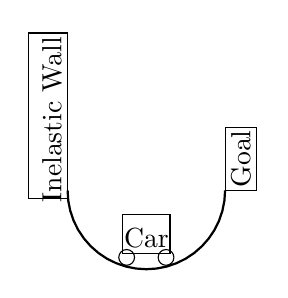
\begin{tikzpicture}
\draw [black,thick,domain=180:360] plot ({cos(\x)}, {sin(\x)});
\node [rotate=90] at (-1.2,0.9) { Inelastic Wall};
\draw (-1.5,-.1) rectangle (-1,2.0);
\node[] at (0,-0.6) { Car};
\draw (-0.3,-0.8) rectangle (0.3,-0.3);
\draw (1,0.0) rectangle (1.4,0.8);

\draw[] (-0.25,-0.85) circle(0.1);
\draw[] (0.25,-0.85) circle(0.1);
\node [rotate=90] at (1.2,0.4) { Goal};
\end{tikzpicture}
\end{center}
\caption{Mountain Car}
\label{mcar}
\end{figure}

In our experiments, we chose $\Ls=\{(x_i^s,y_j^s), 1\leq i,j \leq k_1\}$, where $x_i^s$ and $y_j^s$ were generated according to \eqref{centers} with $k=k_1$. We also fixed $\beta=100$ and $\gamma=2$, and varied $k=5, 7, 9, 11$ and $k_1=30,40,50$, the discount factor was set to $\alpha=0.95$, and $\epsilon=1e^{-5}$. The approximate value function computed by the WMPADP algorithm is shown in Fig.~\ref{ValFunc} and the actual value function is presented in Fig.~\ref{actvalfunc}. The approximate value functions computed in the various settings were used to generate corresponding greedy policies whose performance is shown in Table~\ref{episode}. The performance is evaluated via the number of steps taken by the car to reach the goal using the respective greedy policy.
\FloatBarrier
\begin{table}[H]
\begin{tabular}{|c|c|c|} \hline
$k$ & $k_1$ &Steps to reach the goal\\ \hline	
$5$ &30 &285 \\ \hline
5 &40 &285 \\ \hline
5 &50 &285 \\ \hline

7 &30 &322 \\ \hline
7 &40 &322 \\ \hline
7 &50 &327 \\ \hline

9 &30 &218 \\ \hline
9 &40 &317 \\ \hline
9 &50 &324 \\ \hline

11 &30 &267 \\ \hline
11 &40 &260 \\ \hline
11 &50 &257 \\ \hline
\end{tabular}
\caption{Number of steps taken by the $\emph{Greedy}$ policy}
\label{episode}
\end{table}
The near-optimal policy derived from the actual value function for this problem is known to achieve the goal within $150$ steps \cite{rl}. However, finding the actual value function in this case requires significantly more computation.
\FloatBarrier
\begin{figure}[H]
\begin{tikzpicture}
\begin{axis}
\addplot3 [surf] gnuplot [raw gnuplot] {
set dgrid3d 50,50 spline;
splot 'mfiles/val.dat';       
};
\end{axis}
\end{tikzpicture}
\caption{Actual Value Function Corresponding to the Mountain Car Problem}
\label{actvalfunc}
\end{figure}


\FloatBarrier
\begin{figure*}[H]
\begin{minipage}{1\textwidth}
\resizebox{\columnwidth}{!}{
\begin{tabular}{ccc}
   \begin{tikzpicture}
    \begin{axis}
    \addplot3 [surf] gnuplot [raw gnuplot] {
        set dgrid3d 30,30 spline;
        splot 'mfiles/data730.dat';       
    };
    \end{axis}
    \end{tikzpicture}
&
  \begin{tikzpicture}
    \begin{axis}
    \addplot3 [surf] gnuplot [raw gnuplot] {
        set dgrid3d 40,40 spline;
        splot 'mfiles/data740.dat';       
    };
    \end{axis}
    \end{tikzpicture}
&
  \begin{tikzpicture}
    \begin{axis}
    \addplot3 [surf] gnuplot [raw gnuplot] {
        set dgrid3d 50,50 spline;
        splot 'mfiles/data750.dat';       
    };
    \end{axis}
    \end{tikzpicture}\\
${k=5,k_1=30,V_{\max}=2.83e3 V_{\min}=0.73e3}$ & $k=5,k_1=40,V_{\max}=3.29e3, V_{\min}=0.74e3$	& $k=5,k_1=50,V_{\max}=3.20e3, V_{\min}=0.77e3$\\

   \begin{tikzpicture}
    \begin{axis}
    \addplot3 [surf] gnuplot [raw gnuplot] {
        set dgrid3d 30,30 spline;
        splot 'mfiles/data930.dat';       
    };
    \end{axis}
    \end{tikzpicture}
&
  \begin{tikzpicture}
    \begin{axis}
    \addplot3 [surf] gnuplot [raw gnuplot] {
        set dgrid3d 40,40 spline;
        splot 'mfiles/data940.dat';       
    };
    \end{axis}
    \end{tikzpicture}
&
  \begin{tikzpicture}
    \begin{axis}
    \addplot3 [surf] gnuplot [raw gnuplot] {
        set dgrid3d 50,50 spline;
        splot 'mfiles/data950.dat';       
    };
    \end{axis}
    \end{tikzpicture}\\
${k=7,k_1=30,V_{\max}=2.60e3, V_{\min}=0.45e3}$ &$k=7,k_1=40,V_{\max}=2.83e3, V_{\min}=0.47e3$	&$k=7,k_1=50,V_{\max}=2.80e3, V_{\min}=0.48e3$\\
   \begin{tikzpicture}
    \begin{axis}
    \addplot3 [surf] gnuplot [raw gnuplot] {
        set dgrid3d 30,30 spline;
        splot 'mfiles/data1130.dat';       
    };
    \end{axis}
    \end{tikzpicture}
&
  \begin{tikzpicture}
    \begin{axis}
    \addplot3 [surf] gnuplot [raw gnuplot] {
        set dgrid3d 40,40 spline;
        splot 'mfiles/data1140.dat';       
    };
    \end{axis}
    \end{tikzpicture}
&
  \begin{tikzpicture}
    \begin{axis}
    \addplot3 [surf] gnuplot [raw gnuplot] {
        set dgrid3d 50,50 spline;
        splot 'mfiles/data1150.dat'; 
    };
    \end{axis}
    \end{tikzpicture}\\
${k=11,k_1=30,V_{\max}=2.32e3, V_{\min}=0.18e3}$ &$k=11,k_1=40,V_{\max}=2.42e3, V_{\min}=0.20e3$	&$k=11,k_1=50,V_{\max}=2.42e3, V_{\min}=0.20e3$
\end{tabular}
}
\end{minipage}
\caption{Approximate Value Function for various values of $k$ and $k_1$}
\label{ValFunc}
\end{figure*}




\chapter{Approximate Linear Program}

\chapter{Generalized Reduced Linear Program}
%\section{Curse of Dimentionality}
\emph{Curse-of-Dimensionality} is a term used to denote the fact that the number of states grows exponentially in the number of state variables. Most MDPs arising in practical applications suffer from the curse, i.e., have large number of states and it is difficult to compute $J^*/J_u\in \R^n$ exactly in such scenarios. Approximate dynamic programming (ADP) \cite{lspi,lspe,ALP,wang2014approximate} methods compute an approximate value function $\tilde{J}$ instead of $J^*/J_u$. In order to tackle the curse, ADP methods resort to dimensionality reduction by parameterizing the value function and/or the policy. Value-function based ADP methods form an important subclass of ADP methods whose brief overview is given below.
\section{Value Function Based Approximate Dynamic Programming}
In the value-function based ADP schemes a parameterized family is chosen and the approximate value-function $\tilde{J}$ is picked from the chosen parameterized class.
Once the approximate value function $\tilde{J}$ is computed, a sub-optimal policy $\tilde{u}$ can be obtained as the one-step greedy policy with respect to $\tilde{J}$ by making use of \eqref{subpol}.
The following lemma characterizes the degree of sub-optimality of the greedy policy $\tilde{u}$.
\begin{lemma}\label{subopt}
Let $\tilde{J}$ be the approximate value function and $\tilde{u}$ be as in \eqref{subpol}, then 
\begin{align}
||J^*-J_{\tilde{u}}||_\infty \leq \frac{2}{1-\alpha}||J^*-\tilde{J}||_\infty.
\end{align}
\end{lemma}
\begin{proof}
We know that
\begin{align}
\label{top} (T_{\tilde{u}}) \tilde{J}(s) 	&= g(s)+\alpha \sum_{s'} p_{\tilde{u}(s)} (s,s') \tilde{J}(s'),\\
\label{bot} J_{\tilde{u}}(s)		&=g(s)+\alpha \sum_{s'} p_{\tilde{u}(s)}(s,s')J_{\tilde{u}}(s').
\end{align}
Hence we can write by subtracting \eqref{top} from \eqref{bot} 
\begin{align}
J_{\tilde{u}}-\tilde{J}&=T_{\tilde{u}}\tilde{J}-\tilde{J} +\alpha P_{\tilde{u}}(J_{\tilde{u}}-\tilde{J}),\mb\text{or},\nn\\
J_{\tilde{u}}-\tilde{J}&=(I-\alpha P_{\tilde{u}})^{-1}(T_{\tilde{u}}\tilde{J}-\tilde{J}),\mb \text{hence}\nn\\
||J_{\tilde{u}}-\tilde{J}||_\infty&\leq \frac{1}{1-\alpha}||T_{\tilde{u}}\tilde{J}-\tilde{J}||_\infty.\nn
\end{align}
We know from \eqref{subpol} that $T_{\tilde{u}}\tilde{J}=T\tilde{J}$. Also from the fact that $J^*=TJ^*$ and the contraction property of $T$, we know $||T\tilde{J}-J^*||_\infty\leq \alpha ||\tilde{J}-J^*||_\infty$ and $||T_{\tilde{u}}\tilde{J}-\tilde{J}||_\infty\leq (1+\alpha)||\tilde{J}-J^*||_\infty$. Hence we have
\begin{align}
||J_{\tilde{u}}-J^*||_\infty&=||J_{\tilde{u}}-J^*+\tilde{J}-\tilde{J}||_\infty\nn\\
&\leq  ||J_{\tilde{u}}-\tilde{J}||_\infty+||\tilde{J}-J^*||_\infty\nn\\
&\leq \frac{1}{1-\alpha}||T_{\tilde{u}}\tilde{J}-\tilde{J}||_\infty +||J^*-\tilde{J}||_\infty\nn\\
&\leq \frac{1+\alpha}{1-\alpha}||J^*-\tilde{J}||_\infty +||J^*-\tilde{J}||_\infty\nn\\
&\leq \frac{2}{1-\alpha}||J^*-\tilde{J}||_\infty\nn.
\end{align}
\end{proof}
The quality of any ADP method depends on the approximation guarantees it offers for the quantities $||J^*-\tilde{J}||$ and $||J^*-J_{\tu}||$, where $||\cdot||$ is an appropriate norm. The term  $||J^*-\tilde{J}||$ denotes the error in prediction and $||J^*-J_{\tu}||$ denotes the loss in performance resulting from the sub-optimal policy $\tu$ with respect to the optimal policy $u^*$. Of the two error terms, $||J^*-J_{\tu}||$ is more important because ultimately we are interested in coming up with a useful policy. In the context of ADP methods, the control and prediction problems are said to be addressed when the error terms $||J^*-\tilde{J}||$ and $||J^*-J_{\tu}||$ are bounded by ``small'' constants.\\
\section{Linear Function Approximation}
The most widely used parameterized class to approximate the value-function is the linear function approximator (LFA). Under LFA, the value-function is approximated as $\tilde{J}=\Phi r^*$, with $\Phi=[\phi_1|\ldots|\phi_k]$ being an $n\times k$ feature matrix and $r^*$ is the parameter to be learnt.\\
%ADP methods vary in the way they compute the $\tj$ and $\tu$, and in what follows we present a short overview of some of the chief ADP methods while discussing their successes and shortcomings.
There are two important approaches to value function approximation. Both the approaches start out with a basic solution method and appropriately introduce function approximation in it. The two approaches are:
\begin{enumerate}
\item The Projected Bellman Equation (PBE) which combines the BE and the linear least squares projection operator to project high dimensional quantities onto the subspace of the LFA.
\item The approximate linear programming formulation which introduces the LFA in the linear programming formulation. 
\end{enumerate}


%\section{Approximate Linear Programming}
The LP formulation in \eqref{mdplp} can be represented in short as,
\begin{align}\label{mdplpshort}
\min_{J\in \R^n} &c^\top J\nn\\
\text{s.t}\mb &J\geq T J,\\
\textbf{or}\nn\\
\label{shortalter}
\min_{J\in \R^n} &c^\top J\nn\\
\text{s.t}\mb &EJ\geq H J,\\
\end{align}
where $J\geq TJ$ is a shorthand for the $nd$ constraints in \eqref{mdplp} and $E$ is an $nd\times n$ matrix given by $E=[I,\ldots,I]^\top$, i.e., $E$ is obtained by stacking $d$ identical $n\times n$ identity matrices one over the other. Note that \eqref{mdplpshort} and \eqref{shortalter} are identical programs and differ only in notation. We use notation of type \eqref{mdplpshort} whenever we prefer brevity and we use notation \eqref{shortalter} in some definitions and proof for the sake of clarity.
\begin{comment}
We also follow the convention that constraints $(i-1)\times n+1,\ldots,i\times n$ correspond to the $i^{th}$ action, i.e., the first $n$ constraints correspond to action $1$, and the constraints from $n+1$ to $2n$ correspond to action $2$ and so on. \\
\end{comment}
The approximate linear program (ALP) is obtained by making use of LFA in the LP, i.e., by letting $J=\Phi r$ in \eqref{mdplpshort} and is given as
\begin{align}\label{alp}
\min_{r\in \R^k} &c^\top \Phi r\nn\\
\text{s.t}\mb &\Phi r\geq T \Phi r.
\end{align}
Unless specified otherwise we use $\tr$ to denote the solution to the ALP and $\tj=\Phi \tr$ to denote the corresponding approximate value function. We now state the assumptions and definitions used for the rest of the paper.
\begin{assumption}\label{one}
The first column of the feature matrix $\Phi$ (i.e., $\phi_1$) is $\one \in \R^n$. In other words, the constant function is part of the basis.
\end{assumption}
\begin{assumption}\label{probdist}
$c=(c(i),i=1,\ldots,n)\in \R^n$ is a probability distribution, i.e., $c(i)\geq 0$ and $\sum_{i=1}^n c(i)=1$.
\end{assumption}
\begin{definition}
Given a function $\chi\colon S\ra \R^+$ we define the quantity $\beta_{\chi}$ as
\begin{align}
\beta_{\chi}=\max_{s \in S} \frac{\underset{a \in A}{\max}\big(\alpha\sum_{s'}p_a(s,s')\chi(s')\big)}{\chi(s)}.
\end{align}
\end{definition}
\begin{definition}
The function $\chi$ is then said to be a \emph{Lyapunov} function if $\beta_{\chi}<1$.
\end{definition}
\begin{assumption}\label{lyap}
$\psi\colon S \ra \R^+$ is a Lyapunov function and is present in the column span of the feature matrix $\Phi$.
\end{assumption}
It is straightforward to check that the function $\one$ is a Lyapunov function and trivially is present in the column span of $\Phi$. 
\begin{definition}\label{modlone}
The modified $L_1$-norm is defined as
\begin{align}
||J||_{1,c}=\sum_{s \in S} c(s)|J(s)|,
\end{align}
where $c$ obeys Assumption~\ref{probdist}.
\end{definition}
\begin{definition}\label{modnorm}
The modified $L_\infty$-norm is defined as follows:
\begin{align}
||J||_{\infty,\rho}=\max_{s \in S} \rho(s) |J(s)|,
\end{align}
where $\rho \colon \S \ra \R^+$, $J\in \R^n$.
\end{definition}
In Definition~\ref{modnorm}, the use of the weighting function $\rho$ allows us to measure the error taking into account the relative importance of the various states. A lower value of $\rho(s)$ means that the state $s$ is less important and vice-versa.\\
We recall below Theorem~$4.2$ of \cite{ALP} which bounds the error in the approximate value function.
\begin{theorem}\label{restateval}
Let $\tr$ be the solution to the ALP in \eqref{alp}, $\tilde{J}_c=\Phi \tilde{r}_c$, $\psi$ be a Lyapunov function and $c$ be a distribution as in \eqref{probdist}, then 
\begin{align}
||J^*-\tj||_{1,c}\leq \frac{2c^\top \psi}{1-\beta_{\psi}}\min_{r}||J^*-\Phi r||_{\mn}.
\end{align}
\end{theorem}
We now recall Theorem~$3.1$ of \cite{ALP} that characterizes the loss in performance of the greedy policy.
\begin{theorem}\label{restatepol}
Let $\tilde{u}$ be the greedy policy with respect to the solution $\tj$ of the ALP, then 
\begin{align}
||J^*-J_{\tu}||_{1,c}\leq \frac{1}{1-\alpha}||J^*-\tj||_{1,c'},
\end{align}
where $c'=(1-\alpha)c^\top(I-\alpha P_{\tu})^{-1}$.
\end{theorem}
Theorems~\ref{restateval} and ~\ref{restatepol} together imply that the ALP addresses both the control and prediction problems. Please refer to \cite{ALP} for a more detailed treatment of the ALP.\\
Note that the ALP is a linear program in $k$ ($<<n$) variables as opposed to the LP in \eqref{mdplpshort} which has $n$ variables. Nevertheless, the ALP has $nd$ constraints (same as the LP) which is an issue when $n$ is large and calls for constraint approximation/reduction techniques.

%\section{Constraint sampling}
The most important work in the direction of constraint reduction is constraint sampling \cite{CS} wherein a reduced linear program (RLP) is solved instead of the ALP. While the objective function of the RLP is the same as that of the ALP, the RLP has only $m<<nd$ constraints sampled from the original ALP according to a given probability distribution. The reduced linear program is then given by
\small
\begin{align}\label{rlp}
\min_{J\in \R^n} &c^\top J\nn\\
\text{s.t}\mb &J(s)\geq g_a(s)+\alpha\sum_{s'}p_a(s,s')J(s'), \mb\forall (s,a) \in \I,
\end{align}
\normalsize
where $\I$ is the index set containing the $m$ sampled state-action pairs. Using the index set $\I$ we define an $nd\times m$ matrix $\M$, called the constraint sampling matrix as below.
\begin{definition}\label{csampmat}
Let $\I=\{(s_1,a_1),\ldots,(s_m,a_m)\}$ be the sampled state-action pairs and let $q_i\stackrel{\Delta}{=}s_i+(a_i-1)\times n,\forall i=1,\ldots,m$. Then the constraint sampling matrix associated with the index set $\I$ is given by
\begin{align}
\M(i,j)&=1, \mb\text{if}\mb q_i=j\nn\\
&=0, \mb\text{otherwise}.
\end{align}
\end{definition}
The RLP can then be represented in short as
\begin{align}\label{rlpshort}
\min_{r\in \N} &c^\top \Phi r\nn\\
\text{s.t}\mb & \M^\top E \Phi r \geq \M^\top H \Phi r,
\end{align}
where $\M$ is a constraint sampling matrix as in Definition~\ref{csampmat} and $\N\subset \R^k$ is a bounded set such that $\tr \in \N$. Note that the feasible set of the RLP is a superset of the feasible set of the ALP.\\
The RLP based on constraint sampling has been found to perform well empirically in application domains ranging from controlled queuing networks (see section $6.2$ of \cite{ALP} and section $7$ of \cite{SALP}) to Tetris (see \cite{CST} and section $6$ of \cite{SALP}). However, the theoretical guarantees for the RLP are available only under a restricted setting \cite{CS}. We present the main result of \cite{CS} on constraint sampling, and to that end define the following:
\begin{definition}\label{sampdist}
Given a policy $u$ and Lyapunov function $\psi$ in the column span of $\Phi$, we define probability distributions $\mu_u$, $\mu_{u,\psi}$ and constant $\theta$ as 
% Lyapunov function $\psi$ in the column span of $\Phi$, we define the probability distribution $\mu_{u,\pis}$ as
\begin{align}
\mu^\top&\stackrel{\Delta}{=}(1-\alpha)c^\top (I-\alpha P_u)^{-1},\nn\\
\mu_{u,\psi}(s,a)&\stackrel{\Delta}{=}\frac{\mu_{u}(s) \psi(s)}{\mu_u^\top \psi d},\nn\\
\theta&\stackrel{\Delta}{=}\frac{(1+\beta_{\psi})}{2}\frac{\mu_{u^*}^\top \psi}{c^\top J^*}\sup_{r\in \N}||J^*-\Phi r||_{\mn}.
\end{align}
\end{definition}
We now recall Theorem~$3.1$ of \cite{CS} below.
\begin{theorem}\label{csresult}
Let $\epsilon$ and $\delta$ be scalars in $(0,1)$. Let $u^*$ be the optimal policy and $\I$ an index set containing the $m$ state-action pairs sampled independently according to the distribution $\psi_{u^*,\psi}$, for some Lyapunov function $\psi$, where
\begin{align}
m\geq \frac{16d\theta}{(1-\alpha)\epsilon}\big(k\ln\frac{48d\theta}{(1-\alpha)\epsilon}+\ln\frac{2}{\delta}\big).
\end{align}
Let $\tilde{r}$ be an optimal	solution of the ALP and let $\hat{r}$ be the solution of the corresponding RLP, then with probability at least $1-\delta$, we have
\begin{align}
||J^*-\Phi \hat{r}||_{1,c}\leq ||J^*-\Phi \tilde{r}||_{1,c}+\epsilon||J^*||_{1,c}.
\end{align}
\end{theorem}
\textbf{Motivation for our work:}\\
The result in Theorem~\ref{csresult} has a significant limitation in that the sampling distribution $\mu_{u^*,\psi}$ requires the knowledge of $u^*$. The optimal policy $u^*$ might not be available in practice and hence it would not be possible to even formulate the specific RLP for which the bound in Theorem~\ref{csresult} applies. However, as mentioned before, the RLP has performed reasonably well even when the sampling distribution is not $\mu_{u^*,\psi}$. Thus there is a gap between the theoretical understanding of the RLP and its practical efficacy which merits our attention. The gap also indicates that the RLP might be a special case of a generalized constraint reduction scheme with provable performance guarantees. Understanding such a generalized method would result in an ALP based ADP techinque that would have theoretical performance guarantees while being practically useful. In particular, we wish to answer the following open questions.
\begin{itemize}
\item  As a natural generalization of the RLP, what happens if we define a generalized reduced linear program (GRLP) whose constraints are positive linear combinations of the original constraints of the ALP?
\item Unlike \cite{CS} which provides error bounds for a specific RLP formulated using an idealized sampling distribution, is it possible to provide error bounds for any GRLP (and hence any RLP)?
\end{itemize}
In this paper, we address both of the questions above.

\section{Generalized Reduced Linear Program}
In this section we present the generalized reduced linear program (GRLP) which is obtained by appropriately extending the definition of the RLP. An important property that should carry over from the RLP is that the feasible set of the GRLP should also be a superset of the feasible set of the ALP. A natural way to achieve this is to replace the set of sampled constraints in the RLP by a set of constraints which are obtained as linear combinations of the original constraints of the ALP. Formally, we define the generalized reduced linear program (GRLP) as below:
\begin{align}\label{grlp}
\min_{r\in \chi} &c^\top \Phi r,\nn\\
\text{s.t}\mb & W^\top E\Phi r\geq W^\top H \Phi r, 
\end{align}
where $W \in \R_+^{nd\times m}$ is an $nd\times m$ matrix with all nonnegative entries and $\chi \subset \R^k$ is any bounded set such that $\hj \in \chi$. Thus the $i^{th}$ ($1\leq i\leq m$) constraint of the GRLP is a positive linear combination of the original constraints of the ALP. Constraint reduction is achieved by choosing $m<<nd$. The key difference between the RLP in \eqref{rlpshort} and the GRLP in \eqref{grlp} despite their similar structure is that while $\M$ is a matrix of only zeros and ones, $W$ is a matrix of positive entries alone. Also note that an RLP is trivially a GRLP as well. Unless specified otherwise we use $\hr$ to denote the solution to the GRLP in \eqref{grlp}, $\hj=\Phi \hr$, to denote the corresponding approximate value function and $\hu$ to denote the greedy policy with respect to $\hj$.\par
Note that we want to avoid certain uninteresting and trivial cases of $W$ matrix such as $W=0$ or an entire column of $W$ being zero (which means no constraint is generated with respect to that column). Thus it is intuitive to demand that every column of $W$ should be non-negative and have at least one entry which is strictly positive. Also, normalizing columns of $W$ so that they sum to $1$ does not make any difference to the constraints of the RLP. Keeping these in mind we also assume the following throughout the rest of the paper:
\begin{assumption}\label{wassump}
$W \in \R^{nd\times m}_+$ is a full rank $nd\times m$  matrix (where $m<<nd$) and each of its column sums equals $1$.
\end{assumption}
The above assumption is just a technical condition that eliminates uninteresting choices such as $W=0$ or cases when certain columns of $W$ have all zeros, which implies that the corresponding column generates no constraint.
%\begin{figure}
\centering
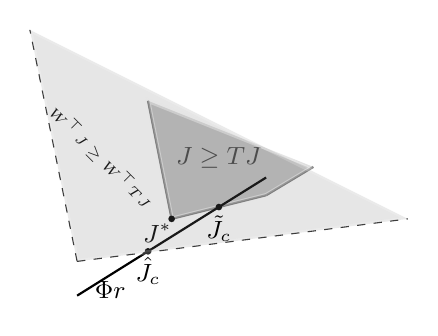
\begin{tikzpicture}[domain=-10:7.7,scale=0.6,font=\small,axis/.style={very thick, ->, >=stealth'}]
\draw[line,thick,-](0.5,3.5)--(1,1);
\draw[line,thick,-](1,1)--(3,1.5);
\draw[line,thick,-](3,1.5)--(4,2.1);
\node[](one) at (2,2.3){\text{$J\geq TJ$}};
\node[rotate=-45](seven) at (-0.5,2.3){\text{\tiny $W^\top J\geq W^\top TJ$}};
\node[](two) at (-0.3,-0.5){\text{$\Phi r$}};
\node[](three) at (0.7,0.7){\text{$J^*$}};
%\draw[line,thick,-](0,0)--(4,2.5);
 \draw [ultra thick, draw=white, fill=gray, opacity=0.5]
       (0.5,3.5)--(1,1)--(3,1.5)--(4,2.1) -- cycle;
\draw[line,thick,-](-1,-0.625)--(3,1.8750);
 \fill (1,1)  circle[radius=2pt];
 \fill (2,1.25)  circle[radius=2pt];
 \fill (0.5,0.3125)  circle[radius=2pt];
\draw[line,dashed,-](-1,0.1)--(6,1);
\draw[line,dashed,-](-1,0.1)--(-2,5);
 \draw [ultra thick, draw=white, fill=gray, opacity=0.2]
       (-1,0.1)--(6,1)--(-2,5) -- cycle;
\node[] (four) at (2,0.8){\text{$\tilde{J}_c$}};
\node[] (six) at (0.5,-0.1){\text{$\hat{J}_c$}};
\end{tikzpicture}
\caption{The outer lightly shaded region corresponds to GRLP constraints and the inner dark shaded region corresponds to the original constraints. The main contribution of the paper is to bound $||J^*-\hat{J}_c||$.}
\label{schematic}
\end{figure}


The rest of the paper develops analytically various performance bounds and our main results provide the following:
\begin{enumerate}
\item A bound for $||J^*-\hj||$, the error between the approximate value function $\hj$ as computed by the GRLP and the optimal value function $J^*$;
\item a bound for $||J^*-J_{\hu}||$, the loss in performance due to the greedy policy $\hu$ measured with respect to the optimal policy; and
\item an important result on constraint sampling.
\end{enumerate}
We achieve the above via two novel $\max$-norm contraction operators namely the least upper bound (LUB) projection operator (denoted by $\Gamma$) and the approximate least upper bound (ALUB) projection operator (denoted by $\hat{\Gamma}$). We bound the error due to constraint approximation by analyzing the fixed points of the operators $\Gamma$ and $\hg$. We first establish our results in the $L_\infty$-norm and then extend the same in a modified $L_\infty$-norm. The schematic in Fig. ~\ref{schematic} provides a pictorial representation of what shall follow in the next three sections.
\FloatBarrier
%\begin{figure}[h!]
\centering
%\resizebox{columnwidth}{}{
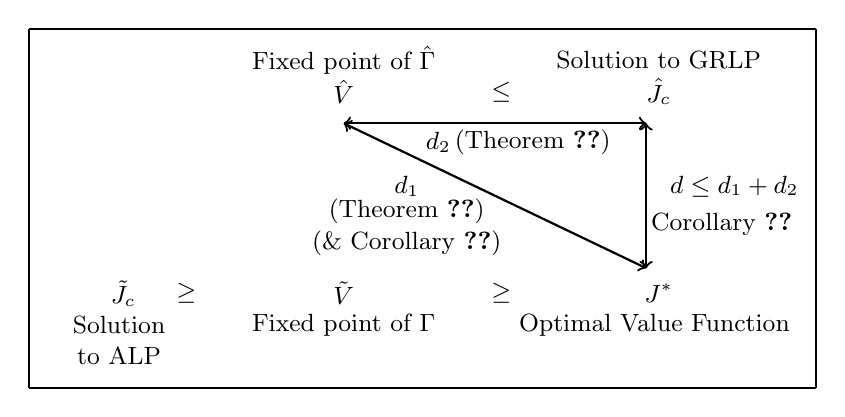
\begin{tikzpicture}[domain=0:7.7,scale=0.8,font=\small,axis/.style={very thick, ->, >=stealth'}]
\draw [line,thick,-] (0,-1)--(0,4.7);
\draw [line,thick,-] (0,4.7)--(12.5,4.7);
\draw [line,thick,-] (12.5,4.7)--(12.5,-1);
\draw [line,thick,-] (0,-1)--(12.5,-1);
\node[](one) at (1.5,0.5) {$\tj$};
\node[](four) at (2.5,0.5) {$\geq$};
\node[](two) at (5,0.5) {$\tv$};
\node[](three) at (10,0.5) {$J^*$};
\node[](five) at (7.5,0.5) {$\geq$};
\node[](six) at (10,3.7) {$\hj$};
\node[](seven) at (5,3.7) {$\hv$};
\node[](eight) at (7.5,3.7) {$\leq$};
\node[](nine) at(1.5,0){\text{Solution }};
\node[](twenty) at(1.5,-0.5	){\text{to ALP }};
\node[](ten) at(5,0){\text{Fixed point of }$\Gamma$};
\node[](eleven) at(10,0){\text{Optimal Value Function }};
\node[](twelve)at (10,4.2){\text{Solution to GRLP}};
\node[](thirteen)at (5,4.2){\text{Fixed point of }$\hg$};
\draw [line,thick,<->] (5,3.2)--(9.8,0.9);
\draw [line,thick,<->] (5,3.2)--(9.8,3.2);
\draw [line,thick,<->] (9.8,3.2)--(9.8,0.9);
\node[](fourteen)at (6,2.2){$d_1$};
\node[](fifteen)at (6.5,2.9){$d_2$};
\node[](sixteen)at (11.2,2.2){$d\leq d_1+d_2$};
\node[](eighteen)at (11,1.6){\text{Corollary~\ref{cmt2}}};
\node[](seventeen)at (8,2.9){\text{(Theorem~\ref{mt2}})};
\node[](fourteen)at (6,1.8){\text{(Theorem~\ref{mt1})}};
\node[](fourteen)at (6,1.3){\text{(\& Corollary~\ref{cmt1})}};
%\node[rotate=-25](fourteen)at (7.5,1.5){\text{(Theorem~\ref{mt1})}};
%\node[draw, circle](two) at (5.5,1) {$s_{n+1}=s'$};
%\draw[->, =>latex](one) edge[bend left=42.5](two);
%\node [above=1.1cm]at (2.8,1.2) {${p_{a_n}(s,s')}$};
%\node [right] at(0,0){$g_{a_n}(s_n)$};
\end{tikzpicture}
%}
\caption{A schematic of the error analysis. Here $d=||J^*-\hj||_{1,c}.$}
\label{schematic}
\end{figure}




\section{Least Upper Bound Projection}\label{sec:lubp}
The least upper bound (LUB) projection operator $\Gamma \colon \R^n \ra\R^n$ is defined as below:
\begin{definition}\label{lubpop}
Given $J\in \R^n$, its least upper bound projection is denoted by $\Gamma J$ and is defined as 
\begin{align}\label{gamdef}
(\Gamma J)(i)\stackrel{\Delta}{=}\underset{j=1,\ldots,k}{\min} (\Phi r_{e_j})(i), \mb \forall i=1,\ldots,n,
\end{align}
where $V(i)$ denotes the $i^{th}$ component of the vector $V\in \R^n$. Also in \eqref{gamdef}, $e_j$ is the vector with $1$ in the $j^{th}$ place and zeros elsewhere, and $r_{e_j}$ is a solution to the linear program in \eqref{lubplp} for $c=e_j$.
\begin{align}\label{lubplp}
r_c\stackrel{\Delta}{=}\min_{r\in \chi} &c^\top \Phi r,\nn\\
\text{s.t}\mb &\Phi r\geq  TJ.
\end{align}
\end{definition}
\vspace{-10pt}
\begin{remark}
\mb\\
\vspace{-10pt}
\begin{enumerate}
\item The definition of LUB operator $\Gamma \colon \R^n \ra \R^n$ involves $n$ associated linear programs.
\item Observe that $\Gamma J\geq TJ$ (follows from the fact that if $a\geq c$ and $b\geq c$, then $\min(a,b)\geq c$, where $a, b, c \in \R$).
\item Given $\Phi$ and $J\in \R^n$, define $\F\stackrel{\Delta}{=}\{\Phi r|\Phi r\geq TJ\}$. Thus $\F$ is the set of all vectors in the span of $\Phi$ that upper bound $TJ$. By fixing $c$ in the linear program in \eqref{lubplp} we select a unique vector $\Phi r_c \in \F$. The LUB projection operator $\Gamma$ picks $n$ vectors $\Phi r_{e_i},i=1,\ldots,n$ from the set $\F$ and $\Gamma J$ is obtained by computing their component-wise minimum.
\item Even though $\Gamma J$ does not belong to the span of $\Phi$, $\Gamma J$ collates the various best upper bounds that can be obtained via the linear program in \eqref{lubplp}.
\item The LUB operator $\Gamma$ in \eqref{gamdef} bears close similarity to the ALP in \eqref{alp}.
\end{enumerate}
\end{remark}
\begin{definition}\label{bestproj}
The LUB projection of $J^*$ is denoted by $\bj=\Gamma J^*$.
\end{definition}
We now characterize the LUB projection operator $\Gamma$ in the following lemmas (all the proofs are presented in the Appendix). As mentioned earlier, the error analysis depends on two $\max$-norm contraction operators the first of which is $\Gamma$. The important result of this section is Theorem~\ref{fxpres} and it relates the fixed point $\tilde{V}$ of $\Gamma$ to $J^*$.
\begin{lemma}\label{bestbnd}
Let $r^*\in \R^k$ be defined as $r^*\stackrel{\Delta}{=}\arg\min_{r\in R^k}||J^*-\Phi r||_\infty$, then 
\begin{align}
||J^*-\bj||_\infty\leq 2||J^*-\Phi r^*||_\infty.
\end{align}
\end{lemma}
\begin{proof}
The result follows from the definition of $\Gamma$ in \eqref{gamdef} and the construction of $V_0$, Assumption~\ref{one}, and the fact that $\Phi r^*+||J^*-\Phi r^*||_\infty \one\geq TJ^*$. To see this, note that
\begin{align}
&\Gamma J^*=\hj \geq J^*,\nn\\
&\Phi r^* +||J^*-\Phi r^*||_\infty\geq TJ^*= J^*.\nn\\
&\text{Thus,}\nn\\
&\Phi r^* +||J^*-\Phi r^*||_\infty\geq \Gamma J^*\geq TJ^*.
\end{align}
\end{proof}

\begin{lemma}\label{gmonotone}
For $J_1, J_2\in \R^n$ such that $J_1\geq J_2$, we have $\Gamma J_1\geq \Gamma J_2$.
\end{lemma}
\begin{proof}
Choose any $i\in \{1,\ldots,n\}$ and let $r^1_{e_i}$ and $r^2_{e_i}$ be solutions to the linear program in \eqref{lubplp} for $c=e_i$ with $J=J_1$ and $J=J_2$ respectively. Since $J_1\geq J_2$, we have $TJ_1\geq TJ_2$ and $e_i^\top \Phi r^1_{e_i} \geq e_i^\top \Phi r^2_{e_i}$, i.e., $(\Phi r^1_{e_i})(i)\geq (\Phi r^2_{e_i})(i)$. The result follows from the fact that $(\Gamma J)(i)=(\Phi r_{e_i})(i),\mb\forall J\in \R^n$, and our choice of $i$ was arbitrary.
\end{proof}
\begin{lemma}\label{lpsol}
Let $A\in \R^{u\times v}$, $b,c\in R^u$, $x_0 \in R^v$ and $b_0=Ax_0$. Then
\begin{align}
\min\{c^\top Ax:Ax\geq b+b_0\} =\min\{c^\top Ax:Ax\geq b\}+c^\top b_0.
\end{align}
\end{lemma}
\begin{proof}
The claim can be shown by a simple change of variables.
\end{proof}
\begin{lemma}\label{gshift}
Let $J_1\in \R^n$ and $t\in \R$ be a constant. If $J_2=J_1+k\one$, then $\Gamma J_2=\Gamma J_1+\alpha t\one$.
\end{lemma}
\begin{proof}
Consider the $i^{th}$ linear programs associated with $\Gamma J_1$ and $\Gamma J_2$. The result follows by using Lemma~\ref{lpsol} with $A=\Phi$, $b=TJ$, $c=e_i$, $b_0=\alpha t\mathbf{1}$ and $x_0=\alpha t e_i$.
\end{proof}
\begin{comment}
\begin{proof}
Choose any $i\in \{1,\ldots,n\}$, let $r^1_{e_i}$ and $r^2_{e_i}$ be solutions to the linear program in \eqref{lubplp} for $c=e_i$ with $J=J_1$ and $J=J_2$ respectively. By Assumption~\ref{one} and Lemma~\ref{shift}, we know that $r^1_{e_i}+\alpha k e_1$ is feasible for the $i^{th}$ linear program associated with $\Gamma J_2$ and we claim that $(\Phi r^2_{e_i})(i)=(\Phi r^1_{e_i})(i)+\alpha k$. On the contrary, if $(\Phi r^2_{e_i})(i)\ne (\Phi r^1_{e_i})(i)+\alpha k$, then $(\Phi r^2_{e_i})(i)< (\Phi r^1_{e_i})(i)+\alpha k$ and since $r^2_{e_i}-\alpha k e_1$ is feasible for the $i^{th}$ linear program associated with $\Gamma J_1$ we will have $(\Phi r^2_{e_i})(i)-k\alpha<(\Phi r^1_{e_i})(i)$. Thus we have arrived at a contradiction because we assumed that $r^1_{e_i}$ is a solution for the $i^{th}$ linear program associated with $\Gamma J_1$. So 
\begin{align}\label{equality}
&(\Phi r^2_{e_i})(i)=(\Phi r^1_{e_i})(i)+\alpha k, \mb\forall i \in \{1,\ldots,n\},\\ \mb &\text{since $i$ was arbitrary}.\nn
\end{align}
From \eqref{equality} and Assumption~\ref{one} it follows that $\Gamma J_2=\Gamma J_1+\alpha k \one$.
\end{proof}
\end{comment}
\begin{theorem}\label{gmaxcontra}
The operator $\Gamma  \colon \R^n\ra \R^n$ obeys the $\max$-norm contraction property with factor $\alpha$.
\end{theorem}
\begin{proof}
Given $J_1,J_2\in \R^n,$ let $\epsilon=||J_1-J_2||_\infty$. Thus,
\begin{align}\label{ineq}
J_2-\epsilon\one\leq J_1\leq J_2+\epsilon \one.
\end{align}
From Lemmas~\ref{gmonotone} and ~\ref{gshift}, we can write
\begin{align}\label{ineq}
\Gamma J_2-\alpha \epsilon\one\leq \Gamma J_1\leq \Gamma J_2+\alpha \epsilon\one.
\end{align}
\end{proof}
\begin{corollary}
The iterative scheme in \eqref{pvi} based on the LUB projection operator $\Gamma$ in \eqref{gamdef} converges to a unique fixed point $\tv$.
\begin{align}\label{pvi}
V_{n+1}&=\Gamma V_n,\mb \forall n\geq 0.
\end{align}
\end{corollary}
\begin{lemma}\label{gfp}
 $\tv$, the unique fixed point of the iterative scheme \eqref{pvi}, obeys $\tv\geq T\tv$.
\end{lemma}
\begin{proof}
Consider the $i^{th}$ linear program associated with $\Gamma \tv$. We know that $\Phi r_{e_i}\geq T \tv,\mb \forall i=1,\ldots, n$. The result follows from noting that $\tv$ is the unique fixed point of $\Gamma $ and that $\tv(i)=\underset{j=1,\ldots,n}{\min}(\Phi r_{e_j})(i)$.
\end{proof}
\begin{lemma}\label{relation1}
 $\tv$, the unique fixed point of the iterative scheme \eqref{pvi}, and the solution $\tj$ to the ALP in \eqref{alp}, obey the relation $\tj\geq\tv\geq J^*$.
\end{lemma}
\begin{proof}
Since $\tv\geq T\tv$ it follows that $\tv\geq J^*$. Let $\Phi r_1, \Phi r_2,\ldots,\Phi r_n$ be solutions to the ALP in \eqref{alp} for $c=e_1, e_2,\ldots,e_n$ respectively. Now consider the iterative scheme in \eqref{pvi} with $V_0(i)=\underset{j=1,\ldots, n}{\min}(\Phi r_j)(i)$. It is clear from the definition of $V_0$ that $\tj(i)\geq\Phi r_i(i)\geq V_0(i),\mb \forall i=1,\ldots,n$. Also from the monotone property of $T$, we have 
\begin{align}\label{lineq}
\Phi r_i&\geq V_0,\nn\\
T\Phi r_i&\geq T V_0,\mbox{we also have}\nn\\
\Phi r_i\geq T\Phi r_i&\geq T V_0,\mb\text{by taking component-wise minimum},\nn\\
V_0&\geq T V_0.
\end{align}
From the first three inequalitites in \eqref{lineq}, $\Phi r_i\geq T \Phi r_i\geq T V_0, \mb\forall i=1\to n$ and hence $V_0\geq TV_0$. Since $V_1=\Gamma V_0$, from the definition of $\Gamma$ in \eqref{gamdef} we have $V_0\geq V_1$, and recursively $V_{n}\geq V_{n+1}, \mb\forall n\geq 0$. So it follows that $\tj\geq V_0\geq V_1\ldots\geq \tv$.
\end{proof}
\begin{theorem}\label{fxpres}
Let $\tv$ be the fixed point of the iterative scheme in \eqref{pvi} and let $\bj$ be the best possible projection of $J^*$ as in Definition~\ref{bestproj}, then
\begin{align}
||J^*-\tv||_\infty\leq \frac{1}{1-\alpha}||J^*-\bj||_\infty.
\end{align}
\end{theorem}
\begin{proof}
Let $\epsilon=||J^*-\bj||_\infty$, and $\{V_n\},n\geq 0$ be the iterates of the scheme in \eqref{pvi} with $V_0=\bj$, then
\begin{align}
||J^*-\tv||_\infty&\leq ||J^*-V_0+V_0-V_1+V_1\ldots-\tv||_\infty\nn\\
&\leq ||J^*-V_0||_\infty+||V_0-V_1||_\infty+\ldots\nn
\end{align}
Since $||V_1-V_0||_\infty=||\Gamma \bj-\Gamma J^*||_\infty\leq\alpha||\bj-J^*||_\infty$, from Theorem~\ref{gmaxcontra},
\begin{align}
||J^*-\tv||_\infty&\leq \epsilon+\alpha\epsilon+\alpha^2\epsilon+\ldots\nn\\
&=\frac{\epsilon}{1-\alpha}.
\end{align}
\end{proof}


\section{Approximate Least Upper Bound Projection}\label{sec:alubp}
We define an approximate least upper bound (ALUB) projection operator which has a structure similar to the GRLP and is an approximation to the LUB operator.
\begin{definition}\label{alubpop}
Given $J\in \R^n$, its approximate least upper bound (ALUB) projection is denoted by $\hg J$ and is defined as 
\begin{align}\label{tgamdef}
(\hg J)(i)\stackrel{\Delta}{=}\underset{j=1,\ldots,k}{\min} (\Phi r_{e_j})(i), \mb \forall i=1,\ldots,n,
\end{align}
where $r_{e_j}$ is a solution to the linear program in \eqref{alubplp} for $c=e_j$, and $e_j$ is the same as in Definition~\ref{lubpop}.
\begin{align}\label{alubplp}
r_c\stackrel{\Delta}{=}\min_{r\in \chi} &c^\top \Phi r,\nn\\
\text{s.t}\mb &W^\top E \Phi r\geq W^\top HJ, W \in \R^{nd\times m}_+ .
\end{align}
\end{definition}
Note that $W$ in \eqref{alubplp} is the same matrix that is used in \eqref{grlp} and satisfies Assumption~\ref{wassump}.
\begin{comment}
The main result of this section is Corollary~\ref{cmt1} which is the stepping stone for the final error bound in Corollary~\ref{cmt2}. The result in this section relates $\hv$, the fixed point of $\hg$ to $J^*$. In Corollary~\ref{cmt2}, we are particularly interested in the term $||\Gamma J^*-\hg J^*||_\infty$ which is precisely the error due to constraint approximation.
\end{comment}
\begin{lemma}\label{tgmonotone}
For $J_1, J_2\in \R^n$ such that $J_1\geq J_2$, we have $\hg J_1\geq \hg J_2$.
\end{lemma}
\begin{proof}
The proof follows from Assumptions~\ref{wassump} and ~\ref{one} using arguments along the lines of Lemma~\ref{gmonotone}.
\end{proof}
\begin{lemma}\label{tgshift}
Let $J_1\in \R^n$ and $t\in \R$ be a constant. If $J_2=J_1+t\one$, then $\hg J_2=\hg J_1+\alpha t\one$.
\end{lemma}
\begin{proof}
The proof follows from Assumption~\ref{wassump} and ~\ref{one}, as well as Lemma~\ref{lpsol} using arguments along the lines of Lemma~\ref{gshift}. In particular, consider the $i^{th}$ linear program corresponding to $\hg J_1$ and $\hg J_2$. Now, the result follows by letting $A=W^\top E \Phi$, $b=W^\top H J$, $c=e_i$, $b_0=\alpha t \mathbf{1}$, $x_0=\alpha t e_i$.
\end{proof}
\begin{theorem}\label{tgmaxcontra}
The operator $\hg \colon \R^n\ra \R^n$ obeys the $\max$-norm contraction property with factor $\alpha$ and the following iterative scheme based on the ALUB projection operator $\hg$, see \eqref{apvi}, converges to a unique fixed point $\hv$.
\begin{align}\label{apvi}
V_{n+1}&=\hg V_n,\mb\forall n\geq 0.
\end{align}
\end{theorem}
\begin{proof}
Follows along similar lines as the proof of Theorem~\ref{gmaxcontra}.
\end{proof}
\begin{lemma}\label{relation2}
The unique fixed point $\hv$ of the iteration in \eqref{apvi} and the solution $\hj$ of the GRLP obey $\hj\geq\hv$.
\end{lemma}
\begin{proof}
Follows in a similar manner as the proof of Lemma~\ref{relation1}. To elaborate, let $\Phi r_1, \Phi r_2,\ldots,\Phi r_n$ be solutions to the GRLP in \eqref{grlp} for $c=e_1, e_2,\ldots,e_n$ respectively. Now consider the iterative scheme in \eqref{apvi} with $V_0(i)=\underset{j=1,\ldots,n}{\min}(\Phi r_j)(i)$. It is clear from the definition of $V_0$ that $\hj(i)\geq\Phi r_i(i)\geq V_0(i), \mb \forall i=1,\ldots,n$. Also from the monotone property of $T$ we have 
\begin{align}
\Phi r_i&\geq V_0,\nn\\
H\Phi r_i&\geq H V_0,\mbox{we also have}\nn\\
E\Phi r_i\geq H\Phi r_i&\geq HV_0,\mb\text{by taking component-wise minimum},\nn\\
E V_0\geq H V_0.
\end{align}
%$\Phi r_i\geq T \Phi r_i\geq T V_0, \mb\forall i=1,\ldots, n$ and hence $V_0\geq TV_0$.
Since $V_1=\hg V_0$, from the definition of $\hg$ in \eqref{gamdef} and the construction of $V_0$, we have $V_0\geq V_1$, and recursively $V_{n}\geq V_{n+1}, \mb\forall n\geq 0$. So it follows that $\hj\geq V_0\geq V_1\ldots\geq \hv$.
\end{proof}
\begin{theorem}\label{mt1}
Let $\hv$ be the fixed point of the iterative scheme in \eqref{apvi} and let $\bj$ be the best possible approximation of $J^*$ as in Definition~\ref{bestproj}, then
\begin{align}
||J^*-\hv||_\infty\leq \frac{||J^*-\bj||_\infty+||\Gamma J^*-\hg J^*||_\infty}{1-\alpha}.
\end{align}
\end{theorem}
\begin{proof}
Let $\epsilon=||J^*-\bj||_\infty$, and $\{V_n\},n\geq 0$ be the iterates of the scheme in \eqref{apvi} with $V_0=\hg J^*$, then
\begin{align}
||J^*-\hg J^*||_\infty&\leq||J^*-\Gamma J^*||_\infty+||\Gamma J^*-\hg J^*||_\infty\nn\\\vspace{10pt}
&= \epsilon+\beta,
\end{align}
where $\beta=||\Gamma J^*-\hg J^*||_\infty$. Now
\begin{align}
||J^*-\hv||_\infty&\leq ||J^*-V_0+V_0-V_1+V_1\ldots-\hv||_\infty\nn\\
&\leq ||J^*-V_0||_\infty+||V_0-V_1||_\infty+||V_1-V_2||_\infty+\ldots\nn\\
&=||J^*-V_0||_\infty+||\hg J^*-\hg V_0||_\infty+\ldots\nn\\\vspace{10pt}
&\leq (\epsilon+\beta)+\alpha(\epsilon+\beta)+\ldots\nn\\
&=\frac{\epsilon+\beta}{1-\alpha}.
\end{align}
\end{proof}

\begin{corollary}\label{cmt1}
Let $\hv$, $\bj$ be as in Theorem~\ref{mt1} and let $r^*\stackrel{\Delta}{=}\arg\min_{r\in \R^k}||J^*-\Phi r||_\infty$, then
\begin{align}
||J^*-\hv||_\infty\leq \frac{2||J^*-\Phi r^*||_\infty+||\Gamma J^*-\hg J^*||_\infty}{1-\alpha}.
\end{align}
\end{corollary}
\begin{proof}
The result is obtained by using Lemma~\ref{bestbnd} to replace the term $||J^*-\bj||_\infty$ in Theorem~\ref{mt1}.
\end{proof}

%\begin{figure*}[t!]
\begin{minipage}{1\textwidth}
\centering
%\resizebox{columnwidth}{2cm}{

\begin{tikzpicture}[domain=-10:7.7,scale=0.7,font=\small,axis/.style={very thick, ->, >=stealth'}]
\draw[line,thick,-] (-21.5,-0.7)--(-21.5,0.8);
\draw[line,thick,-] (-21.5,0.8)--(-3.5,0.8);
\draw[line,thick,-] (-3.5,0.8)--(-3.5,-0.7);
\draw[line,thick,-] (-3.5,-0.7)--(-21.5,-0.7);
\node[](one)at (-20,0.5){\text{Choose right $c$}};
\node[](two)at (-20,0){\text{\& $\Phi$ to}};
\node[](two)at (-19,-0.5){\text{reduce $||J^*-\Phi r^*||_\infty$}};
\draw [line,thick,->] (-18.5,0.5)--(-18,0.5);
\node[](one)at (-16,0.5){\text{Obtain the right ALP}};
\draw [line,thick,->] (-14,0.5)--(-13.5,0.5);
\node[](one)at (-10.2,0.5){\text{Choose a \emph{good} $W$ by computing}};
\node[](one)at (-10.2,0.0){\text{$||\Gamma\bj-\hg \bj||_\infty$ for various $W$s}};
\draw [line,thick,->] (-7.0,0.5)--(-6.5,0.5);
\node[](one)at (-5,0.5){\text{Arrive at the}};
\node[](one)at (-5,0){\text{ right GRLP}};
%\draw[->, =>latex](one) edge[bend left=42.5](two);
%\node[rotate=-25](fourteen)at (7.5,1.5){\text{(Theorem~\ref{mt1})}};
%\node[draw, circle](two) at (5.5,1) {$s_{n+1}=s'$};
%\draw[->, =>latex](one) edge[bend left=42.5](two);
%\node [above=1.1cm]at (2.8,1.2) {${p_{a_n}(s,s')}$};
%\node [right] at(0,0){$g_{a_n}(s_n)$};
\end{tikzpicture}
%}
\caption{A step by step method to arrive at the right GRLP based on the result in \eqref{finalbnd}.}
\label{desmeth}
\end{minipage}
\end{figure*}



\section{A simple bound}
%\vspace{-5pt}
The following lemmas relate the fixed point $\hv$ of $\hg$ to the solution $\hj$ of the GRLP in \eqref{grlp}.
\begin{lemma}\label{srw}
$\hat{r} \in \R^k$ is a solution to GRLP in \eqref{grlp} iff it solves the following program:
\begin{align}\label{grlpeqprog}
\min_{r\in \chi} &||\Phi r-\hv||_{1,c}\nn\\
\text{s.t}\mb & W^\top \Phi r\geq W^\top T \Phi r.
\end{align}
\end{lemma}
\begin{proof}
We know from Lemma~\ref{relation2} that $\hj\geq\hv$, and thus minimizing $||\Phi r-\hv||_{1,c}=\sum_{i=1}^n c(i) |(\Phi r)(i)-\hv(i)|=c^\top \Phi r-c^\top \hv$, is the same as minimizing $c^\top \Phi r$.
\end{proof}
\begin{theorem}\label{mt2}
Let $\hv$ be the solution to the iterative scheme in \eqref{apvi} and let $\hj=\Phi \hr$ be the solution to the GRLP. Let $\bj$ be the best possible approximation to $J^*$ as in Definition~\ref{bestproj}, and $||\Gamma J^* -\hg J^*||_\infty$ be the error due to ALUB projection and let $r^*\stackrel{\Delta}{=}\underset{r\in \R^k}{\arg\min}||J^*-\Phi r||_\infty$, then
\begin{align}
||\hj-\hv||_{1,c}\leq\frac{4||J^*-\Phi r^*||_\infty+||\Gamma J^*-\hg J^*||_\infty}{1-\alpha}.
\end{align}
\end{theorem}
\begin{proof}
Let $\gamma=||J^*-\Phi r^*||_\infty$, then  it is easy to see that
\begin{align}
||J^*-T\Phi r^*||_\infty&=||TJ^*-T\Phi r^*||_\infty\leq\alpha\gamma,\mb\text{and}\nn\\\vspace{10pt}
||T\Phi r^*-\Phi r^*||_\infty&\leq(1+\alpha)\gamma.
\end{align}
From Assumption~\ref{one} there exists $r'\in \R^k$ such that $\Phi r'=\Phi r^*+\frac{(1+\alpha)\gamma}{1-\alpha}\one$ and $r'$ is feasible to the ALP. Now
\begin{align}
||\Phi r'-J^*||_\infty&\leq ||\Phi r^* -J^*||_\infty+||\Phi r'-\Phi r^*||_\infty\nn\\&\leq \gamma+\frac{(1+\alpha)\gamma}{1-\alpha}=\frac{2\gamma}{1-\alpha}.
\end{align}
Since $r'$ is also feasible for GRLP in \eqref{grlp} we have
\begin{align}
||\hj-\hv||_{1,c}&\leq||\Phi r'-\hv||_{1,c}\nn\\\vspace{10pt}
&\leq||\Phi r'-\hv||_\infty\mb\text{(Since $c$ is a distribution)}\nn\\
&\leq||\Phi r'-J^*||_\infty+||J^*-\hv||_\infty.\nn
\end{align}
The result follows from Corollary~\ref{cmt1}.
\begin{comment}
From Corollary~\ref{cmt1} we have
\begin{align}
||\hj-\hv||_{1,c}&\leq\frac{4\gamma+\beta}{1-\alpha}\nn
\end{align}
\end{comment}
\end{proof}\\
\textbf{Prediction Error bound in the $L_\infty$-norm}\\
\begin{corollary}\label{cmt2}
Let $\hj$, $\hv$, $r^*$ and $J^*$ be as in Theorem~\ref{mt2}, then
\begin{align}\label{finalbnd}
||J^*-\hj||_{1,c}\leq\frac{6 ||J^*-\Phi r^*||_\infty+2||\Gamma J^*-\hg J^*||_\infty}{1-\alpha}.
\end{align}
\end{corollary}
\begin{proof}
\begin{align}
||J^*-\hj||_{1,c}&\leq||J^*-\hv||_{1,c}+||\hv-\hj||_{1,c}\nn\\\vspace{10pt}
&\leq||J^*-\hv||_\infty+||\hv-\hj||_{1,c}\nn
\end{align}
The result now follows from Corollary~\ref{cmt1} and Theorem~\ref{mt2}.
\end{proof}
The results presented in Corollary~\ref{cmt2} is in the $L_\infty$-norm. In the next section, we use of Lyapunov functions to provide an improved bound in a modified $L_\infty$-norm.

\section{Improved Bounds}\label{sec:improv}
In this section, we present improved error bounds by making use of Lyapunov functions. 

\begin{comment}
To this end we first define a modified $L_\infty$ norm as follows
\begin{align}
||J||_{\infty,\rho}=\max_{s \in S} \rho(s) |J(s)|,
\end{align}
where $\rho \colon \S \ra \R^+$. The use of weighting function $\rho$ allows us to measure the error taking into account the relative importance of the various states. A lower value of $\rho(s)$ means that the state $s$ is less important and vice-versa.\\
We now define a Lyapunov function
\begin{definition}
Given a function $\chi\colon S\ra \R^+$ we define the quantity $\beta_{\chi}$ as
\begin{align}
\beta_{\chi}=\max_{s \in S} \frac{\underset{a \in A}{\max}\big(\alpha\sum_{s'}p_a(s,s')\chi(s')\big)}{\chi(s)}.
\end{align}
The function $\chi$ is then said to be a \emph{Lyapunov} function if $\beta_{\chi}<1$.
\end{definition}
It is straightforward to check the function $\one$ is a Lyapunov function.\\

Our aim is to bound the error $||\hj-J^*||$ in a suitable modified $L_\infty$ norm. We make the following assumption for analysis in this section
\begin{assumption}\label{lyap}
$\psi\colon S \ra \R^+$ is a Lyapunov function and is present in the column span of the feature matrix $\Phi$.
\end{assumption}
\end{comment}

\begin{lemma}\label{bestbndmn}
Let $r^*\in \R^k$ be defined as $r^*\stackrel{\Delta}{=}\arg\min_{r\in R^k}||J^*-\Phi r||_{\infty,1/\psi}$, then 
\begin{align}
||J^*-\bj||_{\infty,1/\psi}\leq 2||J^*-\Phi r^*||_{\infty,1/\psi}.
\end{align}
\end{lemma}
\begin{proof}
The result follows from the definition of $\Gamma$ in \eqref{gamdef}, Assumption~\ref{lyap} and the fact that $\Phi r^*+||J^*-\Phi r^*||_{\infty,1/\psi} \psi\geq TJ^*$.
\end{proof}

Since most of our analysis in sections~\ref{sec:lubp} and ~\ref{sec:alubp} depended on showing that $\Gamma$ is a contraction map in the $L_\infty$ norm we first show that $\Gamma$ is also a contraction map in the modified $L_\infty$ norm.
\begin{lemma}\label{gshiftmn}
Let $J_1\in \R^n$ and $k\in \R$ be a constant. If $J_2=J_1+k\psi$, then $\Gamma J_2\leq \Gamma J_1+\beta_{\psi} k\psi$.
\end{lemma}
\begin{proof}
The result follows in a similar manner as the proofs for Lemmas~\ref{gshift} and ~\ref{tgshift} by using the result in Lemma~\ref{lpsol}.
\end{proof}
\begin{comment}
\begin{proof}
Choose any $i\in \{1,\ldots,n\}$, let $r^1_{e_i}$ and $r^2_{e_i}$ be solutions to the linear program in \eqref{lubplp} for $c=e_i$ with $J=J_1$ and $J=J_2$ respectively. By Assumption~\ref{one} and Lemma~\ref{shift}, we know that $r^1_{e_i}+\beta_{\psi} k \psi$ is feasible for the $i^{th}$ linear program associated with $\Gamma J_2$ and it follows that 
\begin{align}\label{inequality}
(\Phi r^2_{e_i})(i)&\leq(\Phi r^1_{e_i}(i)+\beta_{\psi} k\psi)(i), \mb\forall i \in \{1,\ldots,n\},\\ \mb &\text{since $i$ was arbitrary}.\nn
\end{align}
The proof follows by noting the fact that $(\Gamma J_2)(i)=(\Phi r^2_{e_i})(i)$.
\end{proof}
\end{comment}
\begin{theorem}\label{gmaxcontramn}
The operator $\Gamma  \colon \R^n\ra \R^n$ is a contraction operator in modified $L_\infty$ with factor $\beta_{\psi}$.
\end{theorem}
\begin{proof}
Given $J_1,J_2\in \R^n$ let $\epsilon=||J_1-J_2||_{\infty,1/\psi}$. Thus
\begin{align}\label{ineq}
J_2-\epsilon\psi\leq J_1\leq J_2+\epsilon \psi.
\end{align}
From Lemmas~\ref{gmonotone} and ~\ref{gshiftmn}, we can write
\begin{align}\label{ineq}
\Gamma J_2-\beta_{\psi} \epsilon\psi\leq \Gamma J_1\leq \Gamma J_2+\beta_{\psi} \epsilon\psi.
\end{align}
Thus
\begin{align}
||\Gamma J_1-\Gamma J_2||_{\infty,1/\psi}\leq \beta_{\psi} ||J_1-J_2||_{\infty,1/\psi}.
\end{align}
\end{proof}
\begin{corollary}\label{hgmaxcontramn}
$\hg$ is also a contraction map in the modified $L_\infty$ norm.
\end{corollary}
\begin{proof}
Follows from arguments similar to Theorem~\ref{gmaxcontramn}.
\end{proof}
\begin{lemma}\label{cmt1mn}
Let $\hv$, $\bj$ be as in Theorem~\ref{mt1} and let $r^*\stackrel{\Delta}{=}\arg\min_{r\in \R^k}||J^*-\Phi r||_{\infty,1/\psi}$ then
\begin{align}
||J^*-\hv||_{\infty,1/\psi}\leq \frac{2||J^*-\Phi r^*||_{\infty,1/\psi}+||\Gamma J^*-\hg J^*||_{\infty,1/\psi}}{1-\beta_{\psi}}.
\end{align}
\end{lemma}
\begin{proof}
The proof follows from Lemma~\ref{gmaxcontramn}, Corollary~\ref{hgmaxcontramn} and by replacing the $||\cdot||_\infty$ norm by $||\cdot||_{\infty,1/\psi}$ in the arguments presented in sections~\ref{sec:lubp} and ~\ref{sec:alubp} leading to Corollary~\ref{cmt1}.
\end{proof}\\
We now recall Lemma~$4.3$ of \cite{ALP}.
\begin{lemma}\label{restate}
Let $\psi$ be a Lyapunov function that belongs to the column span of $\Phi$ , $r \in \R^k$ be an arbitrary vector and let $r'$ be such that
\begin{align}
\Phi r'=\Phi r+||J^*-\Phi r||_{\mn}(\frac{1+\beta_{\psi}}{1-\beta_{\psi}})\psi.
\end{align}
Then $r'$ is feasible for the ALP in \eqref{alp}.
\end{lemma}
\begin{theorem}\label{mt2mn}
Let $\hv$ be the solution to the iterative scheme in \eqref{apvi} and let $\hj=\Phi \hr$ be the solution to the GRLP. Let $\bj$ be the best possible approximation to $J^*$ as in Definition~\ref{bestproj}, and $||\Gamma J^* -\hg J^*||_{\infty,1/\psi}$ be the error due to ALUB projection and let $r^*\stackrel{\Delta}{=}\underset{r\in \R^k}{\arg\min}||J^*-\Phi r||_{\infty,1/\psi}$, then
\begin{align}
||\hj-\hv||_{1,c}&\leq \frac{c^\top \psi}{1-\beta_\psi}(4||J^*-\Phi r^*||_{\mn}
%\nn\\&
+||\Gamma J^*-\hg J^*||_{\mn}).
\end{align}
\end{theorem}
\begin{proof}
Let $\gamma=||J^*-\Phi r^*||_{\infty,1/\psi}$, then by choosing $r'$ as in Lemma~\ref{restate} we have
\begin{align}
||\Phi r'-J^*||_{\mn}&\leq ||\Phi r^*-J^*||_{\mn}+||\Phi r'-\Phi r^*||_{\mn}\nn\\
&=\gamma+\frac{1+\beta_\psi}{1-\beta_\psi}\gamma\nn\\
&=\frac{2}{1-\beta_\psi}\gamma.\nn
\end{align}
Since $r'$ is also feasible for the GRLP in \eqref{grlp} we have
\begin{align}
||\hj-\hv||_{1,c}&\leq||\Phi r'-\hv||_{1,c}\nn\\
&=\sum_{s\in S}c(s)\psi(s)\frac{|\Phi r'(s)-\hv(s)|}{\psi(s)}\nn\\
&\leq c^\top \psi ||\Phi r'-\hv||_{\infty,1/\psi}\nn\\
&\leq c^\top \psi (||\Phi r'-J^*||_{\infty,1/\psi}+||J^*-\hv||_{\infty,1/\psi}).
\end{align}
The result follows from Corollary~\ref{cmt1}.\\
\textbf{Main Result~$1$: Prediction Error bound in modified $L_\infty$-norm}
\end{proof}
\begin{theorem}\label{cmt2mn}
Let $\hj$, $\hv$, $r^*$ and $J^*$ be as in Theorem~\ref{mt2mn}, then
\begin{align}\label{finalbndmn}
||J^*-\hj||_{1,c}&\leq\frac{c^\top\psi}{1-\beta_\psi}(6 ||J^*-\Phi r^*||_{\mn}
%\nn\\&
+2||\Gamma J^*-\hg J^*||_{\mn}).
\end{align}
\end{theorem}
\begin{proof}
\begin{align}
||J^*-\hj||_{1,c}&\leq||J^*-\hv||_{1,c}+||\hv-\hj||_{1,c}\nn\\
&\leq c^\top \psi ||J^*-\hv||_{\mn}+||\hv-\hj||_{1,c}.\nn
\end{align}
The result now follows from Lemma~\ref{cmt1mn} and Theorem~\ref{mt2mn}.
\end{proof}\\

\textbf{Main Result $2$: Control Error bound in modified $L_\infty$-norm}\\
We now bound the performance of the greedy policy $\hu$.
\begin{theorem}\label{polthe}
Let $\hu$ be the greedy policy with respect to the solution $\hj$ of the GRLP and $J_{\hu}$ be its value function. Let $r^*$ be as in Theorem~\ref{mt2mn}, then
\begin{align}\label{polthebnd}
||J_{\hu}-\hj||_{1,c}&\leq 2\big(\frac{c^\top \psi}{1-\beta_{\psi}}\big)^2 \big(6 ||J^*-\Phi r^*||_{\mn}
%\nn\\&
+2||\Gamma J^*-\hg J^*||_{\mn}\big).
\end{align}
\end{theorem}
\begin{proof}
\begin{align}\label{polderv}
||J_{\hu}-\hj||_{1,c}&=||(I-\alpha P_{\hu})^{-1}(T\hj-\hj)||_{1,c}\nn\\
&\leq c^\top(I-\alpha P_{\hu})^{-1}|T\hj-\hj|\nn\\
&\leq c^\top (I-\alpha P_{\hu})^{-1} \psi ||T\hj-\hj||_{\mn}\nn\\
&\leq \frac{c^\top \psi}{1-\beta_{\psi}}||T\hj-\hj||_{\mn}\nn\\
&\leq \frac{c^\top \psi}{1-\beta_{\psi}}||T\hj-TJ^* +J^*- \hj||_{\mn}\nn\\
&\leq \frac{c^\top \psi}{1-\beta_{\psi}}(||T\hj-TJ^*||_{\mn} +||J^*- \hj||_{\mn})\nn\\
&\leq \frac{c^\top \psi}{1-\beta_{\psi}}(1+\beta_{\psi})||J^*- \hj||_{\mn},
\end{align}
where in the second inequality, for $x=(x_1,\ldots,x_n)^\top\in \R^n$, $|x|=(|x_1|,\ldots,|x_n|)^\top\in \R^n$. Now
\begin{align}
||J^*-J_{\hu}||_{1,c}&\leq ||J^*-\hj||_{1,c}+||J_{\hu}-\hj||_{1,c}\nn\\
&\leq c^\top \psi ||J^*-\hj||_{\mn}+c^\top \psi\frac{1+\beta_\psi}{1-\beta_\psi}||J^*- \hj||_{\mn}\nn\\
&=\frac{2c^\top \psi}{1-\beta_{\psi}}||J^*- \hj||_{\mn}.
\end{align}
The result now follows by substituting the value of $||J^*- \hj||_{\mn}$ from Corollary~\ref{cmt2mn}.
\end{proof}
\begin{note}
By letting $\etmn=||\Gamma J^*-J^*+J^*-\hg J^*||_{\mn}\leq 2||J^*-\Phi r^*||_{\infty,1/\psi}+||J^*-\hg J^*||_{\mn}$ (inequality follows from Lemma~\ref{bestbndmn}), we can also modifiy the bounds in \eqref{finalbnd} and \eqref{polthe} as
\begin{align}
\label{loose1}||J^*-\hj||_{1,c}&\leq\frac{c^\top\psi}{1-\beta_\psi}(10 ||J^*-\Phi r^*||_{\mn}
%\nn\\&
+2||J^*-\hg J^*||_{\mn}).\\
\label{loose2}||J_{\hu}-\hj||_{1,c}&\leq 2\big(\frac{c^\top \psi}{1-\beta_{\psi}}\big)^2 \big(10 ||J^*-\Phi r^*||_{\mn}
%\nn\\&
+2||J^*-\hg J^*||_{\mn}\big).
\end{align}
Here the term $||J^*-\hg J^*||$ in \eqref{loose1} and \eqref{loose2} captures the error due to the use of both $\Phi$ and $W$. Though, \eqref{loose1} and \eqref{loose2} might be loser bounds than \eqref{finalbndmn} and \eqref{polthebnd} respectively, the aim here is to capture the error due to function approximation as well as constraint reduction in a single term.
\end{note}


%\section{Result on Constraint Sampling}


\section{Discussion}
In this section we discuss the implications and insights provided by the results presented in Theorems~\ref{cmt2mn} and ~\ref{polthe}.
\subsection{On Error Terms}
\begin{itemize}
\item The error bounds in the main results (Theorems~\ref{cmt2mn} and \ref{polthe}) contain two factors namely
\begin{enumerate}
\item $\min_{r\in \R^k} ||J^*-\Phi r||_{\mn}$,
\item $||\Gamma J^*-\hg J^*||_{\mn}$.
\end{enumerate}
The first factor is related to the best possible approximation that can be achieved with the chosen feature matrix $\Phi$. This term is inherent to the ALP formulation and it appears in the bounds provided by \cite{ALP}.\\
The second factor is related to constraint approximation and is completely defined in terms of $\Phi$, $W$ and $T$, and does not require knowledge of stationary distribution of the optimal policy. It makes intuitive sense since given that $\Phi$ approximates $J^*$, it is enough for $W$ to depend on $\Phi$ and $T$ without any additional requirements.
\item Unlike the result in \cite{CS} which holds only for a specific RLP formulated under ideal assumptions, our bounds hold for any GRLP and as a result for any given RLP. Another interesting feature of our result is that it holds with probability $1$. 
\item A salient feature of the ALP formulation is the use of Lyapunov functions to control/shape the error across the states based on their relative importance. Since the error bounds are in a modified $L_\infty$-norm, the GRLP framework retains this salient feature of the ALP.
\end{itemize}
The fact that both the prediction and control problems can be addressed by the GRLP makes it a complete ADP method, and by addressing the constraint approximation, the GRLP framework is an important addition to the theory of ALP.
\subsection{On Constraint Reduction and Approximation}
We claim the following based on the error bounds that we derived for the GRLP.\\
{Claim $1$)} It is not always necessary to sample constraints according to the stationary distribution of the optimal policy.\\
{Claim $2$)} Constraint approximation is not only restricted to constraint sampling but also can be extended to include linear approximation of the constraints.\\
The following result (Theorem~\ref{st}) supports Claim~$1$ in the above.\\
\textbf{Main Result~$3$: On Constraint Sampling}\\
The error term $\etmn$ gives new insights into constraint sampling. 
\begin{comment}
Before we state our result, we define what we call a \emph{constraint sampling} matrix
\begin{definition}
Let the index set $\I=\{i_1,\ldots,i_m\}$ ( $1\leq i_1<\ldots<i_m\leq n\times d$) denote the constraints to be sampled. We call the $nd\times m$ matrix $W$ to be the corresponding \emph{constraint sampling} matrix and is defined as
\begin{align}
W(i,j)&=1, \mb\text{if}\mb q_i=j\nn\\
&=0, \mb\text{otherwise}
\end{align}
\end{definition}
\end{comment}
\begin{theorem}\label{st}
Let $s\in S$ be a state whose constraint was sampled. Then
\begin{align}\label{sampexp}
|\Gamma J^*(s)-\hg J^*(s)|<|\Gamma J^*(s)-J^*(s)|.
\end{align}
\end{theorem}
\begin{proof}
Let $r_{e_s}$ and $\hat{r}_{e_s}$ be solutions to the linear programs in \eqref{lubplp} and \eqref{alubplp} respectively for $c=e_s$ and $J=J^*$. It is easy to note that $r_{e_s}$ is feasible for the linear program in \eqref{alubplp} for $c=e_s$ and $J^*$, and hence it follows that $(\Phi r_{e_s})(s)\geq (\Phi \hat{r}_{e_s})(s)$. However, since all the constraints with respect to state $s$ have been sampled we know that $(\Phi \hat{r}_{e_s})(s)\geq J^*$. The proof follows from noting that $(\Gamma J^*)(s)=(\Phi r_{e_s})(s)$ and $\hg J^*(s)=(\Phi \hat{r}_{e_s})(s)$.
\end{proof}\\
The expression in \eqref{sampexp} in Theorem~\ref{st} says that the additional error $|\Gamma J^*(s) -\hg J^*(s)|$ due to constraint sampling is less than the original projection error $|\Gamma J^*(s)-J^*(s)|$ due to function approximation. This means that for the RLP to perform well it is enough to retain those states for which the linear function approximation via $\Phi$ is known to perform well. The modified $L_\infty$ norm in \eqref{finalbnd} comes to our rescue to control the error due to those states that are not sampled. Thus the sampling distribution need not be the stationary distribution of the optimal policy as long as it samples the \emph{important} states, an observation that might theoretically explain the empirical successes of the RLP \cite{ALP,CST,SALP}.\\
To understand the implication of Claim~$2$ we need to look at the Lagrangian of the ALP and GRLP in \eqref{lag} and \eqref{lag2} respectively, i.e., 
\begin{align}\label{lag}
\tilde{L}(r,\lambda)=c^\top \Phi r+\lambda^\top (T\Phi r-\Phi r), \\ \label{lag2}\hat{L}(r,q)=c^\top \Phi r+q^\top W^\top (T\Phi r-\Phi r).
\end{align}
The insight that the GRLP is a linear function approximation of the constraints (i.e., the Lagrangian multipliers) can be obtained by noting that $ Wq\approx \lambda$ in \eqref{lag2}. Note that while the ALP employs LFA in its objective function (i.e., use of $\Phi r$), the GRLP employs linear approximation both in the objective function ($\Phi r$) as well as the constraints (use of $W$). Further, $W$ can be interpreted as the feature matrix that approximates the Lagrange multipliers as $\lambda\approx Wq$, where $\lambda \in \R^{nd}, r\in \R^m$. One can show \cite{dolgov} that the optimal Lagrange multipliers are the discounted number of visits to the ``state-action pairs'' under the optimal policy $u^*$, i.e., 
\begin{align}
\lambda^*(s,u^*(s))&=\big(c^\top(I-\alpha P_{u^*})^{-1}\big)(s)\nn\\
				&= \big(c^\top(I+\alpha P_{u^*}+\alpha^2 P_{u^*}^2+\ldots)\big)(s),\nn\\
			\lambda^*(s,a)&=0, \forall a \neq u^*(s),\nn
\end{align}
where $P_{u^*}$ is the probability transition matrix with respect to the optimal policy. Even though we might not have the optimal policy $u^*$ in practice, the fact that $\lambda^*$ is a probability distribution and that it is a linear combination of $\{P_{u^*},P^2_{u^*},\ldots\}$ hints at the kind of features that might be useful for the $W$ matrix.\\
\subsection{Numerical Illustration}
We take up an example in the domain of controlled queues from \cite{ALP} for which the ALP has been known to work well. For this domain, we make use of our results and observations to select various useful $W$ matrices and present their performance.\\
The queuing system consists of $n=10^4$ states and $d=4$ actions. We chose $n=10^4$ because it was possible to solve both the GRLP and the exact LP (the latter with significant effort) so as to enumerate the approximation errors. We hasten to mention that while we could run the GRLP for queuing systems with $n>10^4$ without much computational overhead, solving the exact LP was not possible for $n>10^4$ as a result of which the approximation error could not be computed.\\
\textbf{Queuing Model:}
The queuing model used here is similar to the one in Section~$5.2$ of \cite{ALP}. We consider a single queue with arrivals and departures. The state of the system is the queue length with the state space given by $S=\{0,\ldots,n-1\}$, where $n-1$ is the buffer size of the queue. The action set $A=\{1,\ldots,d\}$ is related to the service rates. We let $s_t$ denote the state at time $t$. The state at time $t+1$ when action $a_t \in A $ is chosen is given by $s_{t+1}= s_{t}+1$ with probability $p$, $s_{t+1}= s_{t}-1$ with probability $q(a_t)$ and $s_{t+1}= s_t$, with probability $(1-p-q(a_t))$. For states $s_t=0$ and $s_t=n-1$, the system dynamics is given by 	$s_{t+1}= s_{t}+1$ with probability $p$ when $s_t=0$ and $s_{t+1}=s_t-1$ with probability $q(a_t)$ when $s_t=n-1$.
The service rates satisfy $0<q(1)\leq \ldots\leq q(d)<1$ with $q(d)>p$ so as to ensure `stabilizability' of the queue. The reward associated with the action $a \in A$ in state $s\in S$ is given by $g_a(s)=-(s+60q(a)^3)$.\\
\textbf{Choice of $\Phi:$} We make use of polynomial features in $\Phi$ (i.e., $1,s,\ldots,s^{k-1}$) since they are known to work well for this domain \cite{ALP}. This takes care of the term $||J^*-\Phi r^*||_\infty$ in \eqref{finalbnd}. \\
\textbf{Selection of $W$:} For our experiments, we choose two contenders for the $W$-matrix and compare them with the ideal sampling matrix $W_i$ (\cite{CS}) and random positive matrix $W_r$. Our choices of the $W$ matrix are as below.\\
{$\mathbf{(i)}$} $W_c$- matrix that corresponds to sampling according to $c$. This is justified by the insights obtained from Theorem~\ref{st} on the error term $\et$, i.e., the idea of selecting the important states.\\
{$\mathbf{(ii)}$} $W_a$ state-aggregation matrix, a heuristic derived using the fact that $\lambda^*$ is a linear combination of $\{P_{u^*},P^2_{u^*},\ldots\}$. Our choice of the $W_a$ matrix to correspond to aggregation of near by states is motivated by the observation that $P^n$ captures $n^{th}$ hop connectivity/neighborhood information.
The aggregation matrix $W_a$ is defined as below: $\forall i=1,\ldots,m$,
\begin{align}\label{wdes}
W_a(i,j)&=1, \mb\forall j\mb\text{s.t}\mb j=(i-1)\times\frac{n}{m}+k+(l-1)\times n, \nn\\&\mb\quad\quad k=1,\ldots,\frac{n}{m}, l=1,\ldots,d,\nn\\
&=0,\mb\text{otherwise}.
\end{align}
We ran our experiments on a moderately large queuing system denoted by $Q_L$ with $n=10^4$ and $d=4$ with $q(1)=0.2$, $q(2)=0.4$, $q(3)=0.6$, $q(4)=0.8$, $p=0.4$ and $\alpha=0.98$. We chose $k=4$ (i.e., we used $1, s,s^2$ and $s^3$ as basis vectors) and we chose $W_a$ \eqref{wdes}, $W_c$, $W_i$ and $W_r$ with $m=50$. We set $c(s)=(1-\zeta) \zeta^s, \mb\forall s=1,\ldots,9999$, with $\zeta=0.9$ and $\zeta=0.999$ respectively. The results in Table~\ref{pref} show that the performance exhibited by $W_a$ and $W_c$ is better by several orders of magnitude over `random' in the case of the large system $Q_L$ and is closer to the ideal sampler $W_i$. Also note that a better performance of $W_a$ and $W_c$ in the larger system $Q_L$ tallies with a lower value of $\et$ in the smaller system $Q_S$.
\FloatBarrier
\begin{table}[H]
%\resizebox{\columnwidth}{!}{
\begin{tabular}{|c|c|c|c|c|}\hline
Error Terms&	$W_i$&	$W_c$& $W_a$& $W_r$ \\\hline
$||J^*-\hj||_{1,c}$ for $\zeta=0.9$& $32$&	$32$& $220$& $5.04\times 10^4$ \\\hline
$||J^*-\hj||_{1,c}$ for $\zeta=0.999$& $110$&	$180.5608$& $82$& $1.25\times 10^7$ \\\hline
\end{tabular}
%}
\caption{Shows values of Error Terms for $Q_L$.}
\label{pref}
\end{table}

\FloatBarrier
\begin{table}[H]
%\resizebox{\columnwidth}{!}{
\begin{tabular}{|c|c|c|c|}\hline
Performance Metric&	$W_i$&	$W_c$& $W_a$ \\\hline
$||J_{\hu}||_{1,c}$ for $\zeta=0.9$& $-441.25$&	$-450.59$& $-446.49$ \\\hline
$||J_{\hu}||_{1,c}$ for $\zeta=0.999$& $-2.0611e+04$&	$-2.0611e+04$& $-2.0612e+04$ \\\hline
\end{tabular}
%}
\caption{Shows performance metrics for $Q_L$. Here $||J^*||_{1,c}=-439.26$ for $\zeta=0.9$ and $||J^*||_{1,c}=-2.0603e+04$ for $\zeta=0.999$   and a random policy yields a total reward of $-1.2661e+03
$.}
\label{pref}
\end{table}
Empirical evidence for the performance of RLP with various sampling distributions can also be found in \cite{CST,CS}.
\subsection{Reinforcement Learning}
Reinforcement Learning (RL) algorithms are useful in scenarios where the system is available in the form of a simulator or only samples can be obtained via direct interaction. In particular, in the RL setting, the model parameters $g$ and $P$ are not known explicitly and the underlying MDP needs to be solved by using sample trajectories. In short, RL algorithms are sample trajectory based solution schemes for solving MDPs whose model information is not known. RL methods learn by filtering out the noisy sample via stochastic approximation and they also employ function approximation in order to handle MDPs with large number of states. Most RL algorithms are sample trajectory based extensions of ADP methods.\\
The RL extension of the ALP formulation has been applied to the optimal stopping problem in \cite{ALP-Bor}. Function approximation is employed to approximate the square root of the Lagrange multipliers. However, since the approximation is not linear, convergence of the resulting RL algorithm cannot be guaranteed. Our results theoretically justify linear function approximation of the Lagrange multipliers, an immediate implication of which is that the RL extension of the ALP can be guaranteed to converge if the updates in \cite{ALP-Bor} use LFA for the Lagrange multipliers instead of a non-linear approximator.
\begin{comment}
We now consider the mountain car example. The problem is to make an under-powered car climb a one-dimensional hill (Fig.~\ref{mcar}), whose position $x$ lies in the interval $[-1.2,0.5]$. There are $3$ actions available to the car, i.e., $A=\{0,1,2\}$. Here $a=0$ and $a=2$ correspond to accelerating to the left and the right respectively. Further, $a=1$ corresponds to no acceleration. The velocity $y$ is limited to $[-0.07,0.07]$. The dynamics is given by
\begin{align}
y_{t+1}&=y_t+0.001 (a_t-1)-0.0025 \cos(3x_t),\\
x_{t+1}&=x_t+y_t.
\end{align}
The state space is continuous with $S=[-1.2,0.5]\times[-0.07,0.07]$ and the state is given by $s=(x,y), x\in [-1.2,0.5], y \in [-0.07,0.07]$. The goal-state is reached once the car crosses the position $x\geq 0.5$. The reward in the goal-state is $100$ and the reward is $0$ in all the other states. 
\FloatBarrier
\begin{figure}[H]
\begin{center}
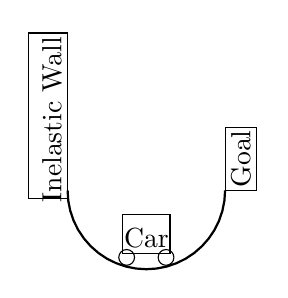
\begin{tikzpicture}
\draw [black,thick,domain=180:360] plot ({cos(\x)}, {sin(\x)});
\node [rotate=90] at (-1.2,0.9) { Inelastic Wall};
\draw (-1.5,-.1) rectangle (-1,2.0);
\node[] at (0,-0.6) { Car};
\draw (-0.3,-0.8) rectangle (0.3,-0.3);
\draw (1,0.0) rectangle (1.4,0.8);

\draw[] (-0.25,-0.85) circle(0.1);
\draw[] (0.25,-0.85) circle(0.1);
\node [rotate=90] at (1.2,0.4) { Goal};
\end{tikzpicture}
\end{center}
\caption{Mountain Car}
\label{mcar}
\end{figure}


\begin{figure}
\centering
\includegraphics[scale=1.0]{careps1.eps}
\caption{Mountain Car}
\label{mcar}
\end{figure}
\end{comment}


\section{Conclusion}
The approximate linear programming (ALP) is an approximate dynamic programming method that addresses the prediction and control problems successfully. However, an important shortcoming of the ALP is that it has large number of constraints, which is tackled in practice by sampling a tractable number of constraints from the ALP to formulate and solve a reduced linear program (RLP). Though RLP has been found to work well empirically in various domains ranging from queues to Tetris games, performance guarantees are available only in the case of a specific RLP formulated under idealized assumptions. Thus there has been a gap in the theory of constraint reduction.\\
In this paper, we introduced a novel framework based on the generalized reduced linear program formulation to study constraint reduction. The constraints of the GRLP were obtained as positive linear combinations of the original ALP. We provided an error bound that relates the optimal value function to the solution of the GRLP. Our error bound contained two terms, one inherent to the ALP formulation and the other due to constraint reduction. We also made qualitative and quantitative observations about the nature of the error term that arose due to constraint reduction. Our analysis also revealed the fact that it is not always necessary to sample according to the stationary distribution of the optimal policy and, in fact, potentially several different constraint sampling/approximation strategies might work. In particular, we also theoretically justified linear function approximation of the constraints. We also discussed the results and provided a numerical example in the domain of controlled queues. To conclude, we observe that by providing a novel theoretical framework to study constraint approximation, this paper provides important results that add to the theory of ALP.





\chapter{Stochastic Approximation and Reinforcement Learning}
\section{Lack of Model Information}

\section{Reinforcement Learning}

\section{Two Timescale Stochastic Approximation}

\section{Actor Critic Algorithms}



\chapter{Stability of Iterates in Two Timescale Stochastic Approximation}
\section{Introduction}
A typical stochastic approximation \cite{kushner} (SA) scheme can be specified as under:
\begin{align}\label{rmsa}
x_{n+1}=x_n+a(n)[h(x_n)+M_{n+1}], n\geq 0,
\end{align}
where the iterates $x_n \in \R^d$, $h\colon \R^d \ra \R^d$, and $M_{n+1}$ are zero-mean noise terms and $a(n)$ are diminishing step sizes. The earliest and most representative example of an SA scheme is the 
Robbins-Monro (RM) algorithm, an iterative procedure to compute the zeros of a function using only 
its noisy observations. Here, $h$ is the function whose unique zero say $x^* \in \R^d$ needs to be 
computed and at any point $x_n$, the value of the function $h(x_n)$ is corrupted by an additive noise 
$M_{n+1}$. Other instances of SA schemes are the stochastic gradient schemes wherein $h$ is the 
gradient of some other function $f\colon \R^d \ra \R$, i.e., $h(x)=\nabla f(x)$. Stochastic gradient 
schemes are found to be useful in actor-critic \cite{NAC,IAC,KAC,BAC,BSPSA,Pet-Sch,ALP-Bor,SB1} and policy gradient \cite{Bax-Bar,Amari,SMSM,Kak,SP} reinforcement learning algorithms as well as stochastic optimization algorithms \cite{SPSA,TTSPSA,SB-VB,Mar-Tsit,SB-VB2,SB3,BTS,BO,BADA}.\\
\indent The conditions under which the above scheme converges have been studied widely (\cite{kushner,SA}) 
in the literature. In general, analysis of SA schemes involves two important steps namely,
\begin{enumerate}
\item establishing $\emph{stability}$ of the iterates $x_n$, i.e., showing that 
$\sup_n \parallel x_n\parallel <\infty$ with probability one, and  \label{stb}
\item establishing $\emph{convergence}$ to a desired solution $x^*$, i.e., showing that 
$x_n \rightarrow x^*$ almost surely as $n \rightarrow \infty$. \label{conv}
\end{enumerate}
%Often \ref{stb} is required to show \ref{conv} (\cite{SA}).
In situations where stability of iterates cannot be established analytically, a common procedure 
is to pick a suitable compact subset of the parameter space onto which one would projects the iterates, 
thereby ensuring their boundedness, i.e., $\sup_n \parallel x_n\parallel <\infty$.\\
\indent The ODE method (\cite{SA,BMSTAB}) is a useful analytical tool to study the stability as well as 
convergence of the stochastic iterates. In the ODE method, one considers \eqref{rmsa} to be a 
$\emph{noisy-discretized}$ version of the ODE,
\begin{align}\label{odebasic}
\dot{x}(t)=h(x(t)).
\end{align}
An important notion associated with the ODE method is that of $\emph{timescale}$ that is
defined using the quantity $t(n)=\sum_{m=0}^{n-1} a(m),\mb n\geq 1$. Let $\phi(t,x), t\geq 0$ 
denote the trajectory of \eqref{odebasic} with initial condition $x(0)=x$. When $\sup_n\parallel
x_n\parallel <\infty$, 
the trajectory $\phi(t,x)$ sampled at instants $t(n)$, i.e., $\{\phi(t(n),x_0), n\geq 0\}$ approximates the 
iterates ${x_n}$ (Lemma~$1$, Chapter $2$,\cite{SA}). The SA scheme can then be shown to converge to a 
compact connected internally chain transitive invariant set of the ODE in \eqref{odebasic}. 
Thus the convergence of iterates in the SA scheme \eqref{rmsa} can be understood by looking at the 
asymptotic equilibria of the ODE in \eqref{odebasic}.\\
\indent
The ODE method can also be used to establish the stability of iterates $\{x_n\}$ which involves 
understanding the behavior of \eqref{rmsa} when $\parallel x_n\parallel$ gets larger. The idea is to observe
the evolution of the continuously interpolated trajectory obtained from the iterates $\{x_n\}$ every 
$T$ instants and then rescaling it to the unit ball if the trajectory goes out of it. 
The rescaled iterates $\{\tilde{x}_n\}$ then differ from the original iterates $\{x_n\}$ only by a 
constant factor. The rescaled iterates track the rescaled ODE,
\begin{align}
\dot{x}(t)=h_{c}(x(t)), \text{where}\mbox{ } h_c(x)\stackrel{def}{=}\frac{h(cx)}{c}, \forall c\geq 1.
\end{align}
As $c \ra \infty$, one obtains the following $\emph{limiting}$ ODE (assuming the limit exists):
\begin{align}\label{lode}
\dot{x}(t)=h_\infty(x(t)), \text{where} \mbox{ } h_\infty(x)=\lim_{c \ra \infty} h_c(x).
\end{align}
When the ODE \eqref{lode} is globally asymptotically stable to the origin, \cite{BMSTAB} shows that 
$\sup_n \parallel x_n\parallel <\infty$ almost surely. This is because outside a set of zero probability,
as $\parallel x_n\parallel$ grows larger, the scaling factor tends to $\infty$ and 
$\tilde{x}_n$ can be approximated 
by the trajectory of the limiting ODE \eqref{lode}. Since the ODE \eqref{lode} is stable to the origin, 
the scaled iterates $\{\tilde{x}_n\}$ fall back to the origin. The stability of $\{x_n\}$ then follows 
upon noting that these iterates differ from $\tilde{x}_n,n\geq 1$ only by a scaling factor.\\
\indent The SA scheme in \eqref{rmsa} is a $\emph{single}$ timescale stochastic approximation scheme. 
A two-timescale stochastic approximation scheme \cite{TTSAP,BADA,SB-VB2,TTSPSA,BO,BTS} 
is as under:
\begin{subequations}\label{ttsaintro}
\begin{align}
\label{frec} x_{n+1}&=x_n+a(n)[h(x_n,y_n)+M^{(1)}_{n+1}],\\
\label{srec} y_{n+1}&=y_n+b(n)[g(x_n,y_n)+M^{(2)}_{n+1}], 
\end{align}
\end{subequations}
where, $x_n \in \R^{d_1}, y_n \in \R^{d_2}$, $a(n)$ and $b(n)$ are both diminishing step-size schedules 
except that $\frac{b(n)}{a(n)} \rightarrow 0$ as $n\rightarrow \infty$. 
The two timescales here are, the $\emph{slower}$, corresponding to $t^s(n)=\sum^{n-1}_{m=0} b(m)$, 
and the $\emph{faster}$,  corresponding to  $t^f(n)=\sum^{n-1}_{m=0} a(m)$ respectively, on which 
the two recursions proceed. The terms $\emph{faster}$ and $\emph{slower}$ signify the rates of growth 
of $t^f(n)$ and $t^s(n)$ respectively. Many iterative schemes might involve calls to subroutines which 
themselves are iterative in nature. Thus the $\emph{outer}$-loop in such schemes must typically wait for 
the iterates in the $\emph{inner}$-loop to converge before proceeding to its next step. 
Instead, the same effect can also be achieved by a two-timescale recursion with outer and inner loop 
iterates on the slower and faster timescales respectively. The condition $\frac{b(n)}{a(n)} \ra 0$ 
ensures that the slower timescale iterates do not move much compared to the faster timescale iterates, 
thereby producing the effect equivalent to that of a $\emph{nested}$-loop. As a result,
multi-timescale stochastic approximation is commonly used in algorithms that involve estimation of 
$\emph{nested}$ quantities \cite{NAC,IAC,KAC,TTSAP,SB-VB2,BTS}. Study of two timescale SA schemes is 
also important as it is easy to extend the arguments made for two timescale recursions to those with 
even more timescales.\\
\indent Under the assumption that $\sup_n\parallel x_n\parallel <\infty$, $\sup_n\parallel y_n\parallel
<\infty$, the ODE method can 
be applied to establish the convergence of iterates in \eqref{ttsaintro}, see \cite{TTSAP} 
and Chapter~$6$, \cite{SA}. In this paper, we provide {\em the first} conditions in the literature
that imply stability of the iterates in \eqref{ttsaintro}. These are conditions that imply 
$\sup_n\parallel x_n\parallel <\infty$ and $\sup_n\parallel y_n\parallel
<\infty$ with probability one. Stability results 
for the single timescale recursions, see \cite{BMSTAB} and Chapter $3$ of \cite{SA}, cannot be applied 
directly to the two-timescale scheme in \eqref{ttsaintro}, because the iterates $\{x_n\}$ and $\{y_n\}$ 
are coupled and they evolve along separate timescales. Nonetheless, while our analysis resembles 
\cite{SA,TTSAP} 
in that we study scaled ODEs, it differs considerably from \cite{SA} in that we study two separate 
sets of scaled ODEs for the two different timescales. Since the iterates $x_n$ evolve on the faster 
timescale, it is natural to first characterize the growth of $\{x_n\}$ before studying the stability
of $\{y_n\}$. So, we first study the following scaled ODE and its limiting version:
\begin{align}
\label{hcf} \dot{x}(t)&={h}_c(x(t),y), \text{where}\mbox{ } {h}_c(x,y)\stackrel{def}{=}\frac{h(cx,cy)}{c}, 
c \geq 1,\\
\label{hif} \dot{x}(t)&=h_\infty(x(t),y), \text{where}\mbox{ } {h}_\infty(x,y)=\lim_{c \ra \infty}h_c(x,y).
\end{align}
Equations \eqref{hcf} and \eqref{hif} also allude to the fact that the slower timescale iterates 
appear to be constant, i.e., $y(t)\equiv y$ $\forall t$, when viewed from the faster timescale 
\cite{SA}.\\
Under the assumption that the limiting ODE \eqref{hif} has a unique globally asymptotically stable 
equilibrium $\lambda_\infty(y)$, where $\lambda_\infty \colon \R^{d_2} \ra \R^{d_1}$
is a Lipschitz continuous map with $\lambda_\infty(0)=0$, we show that $\parallel x_n\parallel
\leq K^*(1+\parallel y_n\parallel)$ 
for some $K^*>0$. Subsequently, we analyze the slower recursion using the following ODE:
\begin{align}\label{gc} 
\dot{y}(t)=g_c(y(t)), \text{where } \mbox{ } g_c(y)=\frac{g(c\lambda_\infty(y),cy)}{c}.
\end{align}
We show that $\sup_n \parallel y_n\parallel <\infty$ with probability one, when the limiting 
ODE $\dot{y}(t)=g_\infty(y(t))$ (with $g_\infty(y)=\underset{c\ra\infty}{\lim}g_c(y)$) is stable 
to the origin. By making use of the fact that $\parallel x_n\parallel \leq K^*(1+\parallel y_n\parallel)$ 
(see above), 
we establish the stability of two timescale SA iterates given in \eqref{ttsaintro}.\\
\indent The paper is organized as follows. In section~\ref{oderes} we summarize certain results 
(mostly from \cite{SA,TTSAP}) regarding the scaled ODEs that will be used in our arguments. 
In sections~\ref{faster} and ~\ref{slower}, we present the analysis for the faster and slower 
timescale recursions, respectively. In section~\ref{example}, we apply our analysis to establish 
the stability of iterates in a two-timescale stochastic approximation algorithm arising in an 
application in reinforcement learning. Conclusions are provided in section~\ref{disc}. 
Finally, an Appendix at the end presents the Gronwall inequalities that are used in the proofs 
and a result whose proof follows along the lines of a similar result in \cite{SA}.


\section{Results for the Scaled ODE}\label{oderes}
Let $u \colon\R^{d_1+d_2}\ra\R^{d_1}$ be a Lipschitz map, i.e., there exists $L>0$ such that 
$\parallel u(x_1)-u(x_2)\parallel \leq L\parallel x_1-x_2\parallel, x_1,x_2\in \R^{d_1+d_2}$. 
Let $\eta^{q(t)}(t,p)$ denote the solution to the ODE
\begin{align}\label{auto}
\dot{p}(t)=u(p(t),q(t)), \mb t \geq 0,
\end{align}
with initial condition $p\in \R^{d_1}$ and the external input $q(t) \in \R^{d_2}$. The superscript $q(t)$ in $\eta^{q(t)}(t,p)$ is to be understood as a symbol that indicates the fact that the external input is $q(t)$. 
%Thus $q(t)$ in $\eta^{q(t)}(t,p)$ is not to be interpreted as a function of time. 
We denote by $\eta^q(t,p)$ the solution to the ODE
\begin{align}\label{autofix}
\dot{p}(t)=u(p(t),q), \mb t \geq 0.
\end{align}
Thus, in \eqref{autofix}, $q(t)=q, \forall t\geq 0$ for some $q\in \R^{d_2}$. Hence, in \eqref{autofix},
the external input is a constant as opposed to being a function of time as with \eqref{auto}.
Let $B(p_0,r)=\{p\colon \parallel p-p_0\parallel \leq r\}$ denote the closed ball of radius $r$ 
around $p_0$. The 
lemma below is a generalization of Lemma~$1$, Chapter $3$ of \cite{SA}.
\begin{lemma}\label{attract}
Let $K\subset \R^{d_1}$ be a compact set and $q\in \R^{d_2}$ be a fixed external input to the ODE in 
\eqref{autofix}. If this ODE has a unique globally asymptotically stable equilibrium (a.s.e) 
$\lambda(q) \in \R^{d_1}$, then given any $\delta>0$, there exists a $T_\delta>0$ such that for all 
initial conditions $p \in K$, we have
\begin{align}
 \eta^q(t,p) \in B(\lambda(q),\delta), \forall t\geq T_\delta.\nn
\end{align}
\end{lemma}
\begin{proof}
Since $\lambda(q)$ is the unique globally a.s.e, it is Lyapunov stable. Hence, there exists a 
$\delta'>0$ (assume $\delta'<\delta$ without loss of generality) such that any trajectory starting 
in $B(\lambda(q),\delta')$ stays within $B(\lambda(q),\delta)$ forever, i.e., for any $s\geq 0$,
\begin{align}
\eta^q(s,p)\in B(\lambda(q),\delta') \Rightarrow \eta^q(t,p) \in B(\lambda(q),\delta), \mb \forall t \geq s.
\end{align}
Let $p \in K$ be a given initial condition and since $\lambda(q)$ is a globally a.s.e, there exists a 
$T_{p}$ such that $\eta^q(T_p,p)\in B(\lambda(q),\delta'/2)$. Let $p'$ be some other initial condition, 
then for $t \in [0,T_p]$,
\begin{align}
\eta^q(t,p)&=p+\int_0^t u(\eta^q(s,p),q)ds,\nn\\
\eta^q(t,p')&=p'+\int_0^t u(\eta^q(s,p'),q)ds.\nn
\end{align}
Subtracting the two equations above, we get
\begin{align}
\parallel \eta^q(t,p)-\eta^q(t,p')\parallel &\leq \parallel p-p'\parallel +L\int_0^t \parallel
\eta^q(s,p)-\eta^q(s,p')\parallel ds\nn\\
&\leq \parallel p-p'\parallel e^{LT_p}, \forall t \in [0,T_p].
\end{align}
The last inequality above follows from the Gronwall inequality (see Appendix). Given any $p\in K$, one can always choose $p'$ close enough to $p$ such that $\parallel p-p'\parallel e^{LT_p}<\delta'/2$ and 
$\eta^q(T_p,p') \in B(\lambda(q),\delta')$. Thus there is a neighborhood $U_p$ of $p$ such that for all $p' \in U_p$, $\eta^q(t,p') \in B(\lambda(q),\delta'), \forall t\geq T_p$. Now $\underset{p\in K}{\cup} U_p$ is a cover for $K$ and since $K$ is compact there exists a finite sub-cover $\{U_{p_1}, \ldots,U_{p_n}\}$ such that $K \subset \cup_{i=1}^nU_{p_i}$. 
Let $T_\delta=\max\{T_{p_i}, i=1,\ldots,n\}$, then for any $p
\in K$,
\begin{align}
\eta^q(T_\delta,p)\in B(\lambda(q),\delta') \Rightarrow \eta^q(t,p) \in B(\lambda(q),\delta), \mb \forall t \geq T_\delta.
\end{align}
\end{proof}
\begin{assumption}\label{scalefns}
Let functions $u_c \colon \R^{d_1+d_2} \ra \R^{d_1}, c\geq 1$ be a family of Lipschitz continuous functions 
with Lipschitz constant $L$. Let $u_c \ra u_\infty$ as $c \ra \infty$ uniformly on compacts to some 
$u_\infty \in \mathcal{C}(R^{d_1+d_2})$.
\end{assumption}
\begin{lemma}
$u_\infty\colon \R^{d_1+d_2}\ra \R^{d_1}$ is also a Lipschitz continuous function with Lipschitz constant $L$.
\end{lemma}
\begin{proof}
Given $x_1,x_2 \in \R^{d_1+d_2}$, we have
\begin{align}
\parallel u_\infty(x_1)-u_\infty(x_2)\parallel &\leq\parallel u_\infty(x_1)-u_c(x_1)\parallel
+\parallel u_c(x_1)-u_c(x_2)\parallel +\parallel u_c(x_2) -u_\infty(x_2)\parallel \nn\\
&\leq 2\epsilon(c)+L\parallel x_1-x_2\parallel,
\end{align}
where since $c$ is arbitrary, we let $c\ra \infty$, whereby $\epsilon(c)\ra 0$. The second inequality above 
follows from Assumption~\ref{scalefns}. So we have
\begin{align}
\parallel u_\infty(x_1)-u_\infty(x_2)\parallel \leq L\parallel x_1-x_2\parallel.
\end{align}
\end{proof}
Let $\eta^{q(t)}_c(t,p)$ and $\eta^{q(t)}_\infty(t,p)$ be solutions\footnote{When the external input is 
constant, i.e., $q(t)=q, \forall t\geq 0$, we denote the same by $\eta^{q}_c(t,p)$ and $\eta^{q}_\infty(t,p)$,
respectively.} to the ODEs \eqref{odec} and \eqref{odei}, respectively, with $p(0)=p$. 
\begin{align}\label{odec}
\dot{p}(t)=u_c(p(t),q(t)),
\end{align}
\begin{align}\label{odei}
\dot{p}(t)=u_\infty(p(t),q(t)).
\end{align}
Lemma~\ref{near} below is a generalization of Lemma~$2$, Chapter~$3$ of \cite{SA}.
\begin{lemma}\label{near}
Let $p \in \R^{d_1}$, $q\in \R^{d_2}$, $[0,T]$ be a given time interval and $r>0$ be a small positive constant. Let $q'(t) \in B(q,r), \mb \forall t\in [0,T]$, then 
\begin{align}
\parallel \eta^{q'(t)}_c(t,p)-\eta^q_\infty(t,p)\parallel \leq (\epsilon(c)+Lr)Te^{LT}, 
\mb \forall t \in [0,T], \nn
\end{align}
where $\epsilon(c)$ is independent of $p$ and $q$ and $\epsilon(c) \ra 0$, as $c \ra \infty$.
\end{lemma}
\begin{proof}
\begin{align}
\eta^{q'(t)}_c(t,p)&=p+\int_0^t u_c(\eta^{q'(t)}_c(s,p),q'(t))ds,\nn\\
\eta^q_\infty(t,p)&=p+\int_0^t u_\infty(\eta^q_\infty(s,p),q)ds,
\end{align}
and hence
\begin{align}
\parallel \eta^{q'(t)}_c(t,p)-\eta^q_\infty(t,p)\parallel \leq \int_0^t \parallel u_c(\eta^{q'(t)}_c(s,p),
q'(t))-u_\infty(\eta^q_\infty(s,p),q)\parallel ds.
\end{align}
Since $u_c$ and $u_\infty$ are Lipschitz continuous, we have
\begin{align}
&\parallel u_c(\eta^{q'(t)}_c(s,p),q'(t))-u_\infty(\eta^q_\infty(s,p),q)\parallel \nn\\
&\leq \parallel u_c(\eta^{q'(t)}_c(s,p),q'(t))-u_c(\eta^q_\infty(s,p),q'(t))\parallel \nn\\
&+\parallel u_c(\eta^q_\infty(s,p),q'(t))-u_\infty(\eta^q_\infty(s,p),q'(t))\parallel \nn\\
&+\parallel u_\infty(\eta^q_\infty(s,p),q'(t))-u_\infty(\eta^q_\infty(s,p),q)\parallel \nn\\
&\leq L\parallel \eta^{q'(t)}_c(s,p)-\eta^q_\infty(s,p)\parallel +\epsilon(c)+L\parallel
q-q'(t)\parallel \nn\\
&\leq L\parallel \eta^{q'(t)}_c(s,p)-\eta^q_\infty(s,p)\parallel +\epsilon(c)+Lr,\nn
\end{align}
where $\epsilon(c)$ is independent of $p \in K$, and $\epsilon(c) \ra 0$ as $c \ra \infty$. The last line 
follows from the fact that $q'(t)\in B(q,r), \mb \forall t\in [0,T]$. Now we have
\begin{align}
\parallel \eta^{q'(t)}_c(s,p)-\eta^q_\infty(s,p)\parallel \leq \epsilon(c)T+Lr T +L\int^t_0\parallel
\eta^{q'(t)}_c(s,p)-\eta^q_\infty(s,p)\parallel ds.
\end{align}
The claim now follows from the Gronwall inequality.
\end{proof}
\begin{lemma}\label{within}
Let $q\in \R^{d_2}$ and let $\lambda_\infty(q)$ be the unique globally asymptotically stable equilibrium 
of \eqref{odei}. Given any $\epsilon >0$ and $T>0$, there exist $c_{\epsilon,T}> 0 $, $\delta_{\epsilon,T} 
> 0$ and $r_{\epsilon,T} > 0$ such that $\forall t\in [0,T), \forall p \in 
B(\lambda_\infty(q),\delta_{\epsilon,T}), \mb \forall c>c_{\epsilon,T}$ and external input $q'(s)$ with 
\begin{align}
q'(s) \in B(q,r_{\epsilon,T}), s\in [0,T],
\end{align}
we have
\begin{align}
\eta^{q'(t)}_c(t,p) \in B(\lambda_\infty(q),2\epsilon), \forall t \in [0,T].
\end{align}
\end{lemma}
\begin{proof}
Given any $\epsilon >0$, it follows from Lyapunov stability that there exists $\delta_{\epsilon,T}>0$ such that any trajectory of \eqref{odei} starting in $B(\lambda_\infty(q),\delta_{\epsilon,T})$ stays within the ball $B(\lambda_\infty(q),\epsilon)$. Without loss of generality we can assume $\delta_{\epsilon,T}<\epsilon$. From Lemma~\ref{near} we know that there exist $c_{\epsilon,T}$ and $r_{\epsilon,T}$ such that
\begin{align}
\parallel \eta^{q'(t)}_c(t,p)-\eta^{q}_\infty(t,p)\parallel&\leq \epsilon.
\end{align}
Hence, $\forall t \in [0,T],\mb \forall q'(t)\in B(q,r_{\epsilon,T}), \mb\forall p \in B(\lambda_\infty(q),\delta_{\epsilon,T})$ and $\forall c> c_{\epsilon,T}$,
\begin{align}
\parallel \eta^{q'(t)}_c(t,p)-\lambda_\infty(q)\parallel &\leq \parallel \eta^{q'(t)}_c(t,p)-\eta^{q}_\infty
(t,p)\parallel + \parallel \eta^{q}_\infty(t,p)-\lambda_\infty(q)\parallel \nn\\
&\leq \delta/2+\epsilon\nn\\
&\leq 2\epsilon.
\end{align}
The claim follows.
\end{proof}
\begin{lemma}\label{neartraj}
 Let $p\in B(0,1) \subset \R^{d_1}$, $q\in K'\subset\R^{d_2}$ and let $\lambda_\infty(q)$ be the unique globally asymptotically stable equilibrium of \eqref{odei}. Then, given $\epsilon > 0$, there exists $c_\epsilon\geq 1$, $r_{\epsilon}>0$ and $T_\epsilon>0$ such that for any external input $q'(s)$ satisfying
\begin{align}\label{qcond}
q'(s) \in B(q,r_{\epsilon}), \forall s\in [0,T],
\end{align}
we have
\begin{align}
\parallel \eta^{q'(t)}_c(t,p)-\lambda_\infty(q)\parallel \leq 2\epsilon, \forall t\geq T_\epsilon, 
\forall c>c_\epsilon.
\end{align}
\end{lemma}
\begin{proof}
Given any $\epsilon >0$, it follows from Lyapunov stability that there exists $\delta>0$ such that any 
trajectory of \eqref{odei} starting in $B(\lambda_\infty(q),\delta)$ stays within the ball 
$B(\lambda_\infty(q),\epsilon)$. Without loss of generality we can assume $\delta<\epsilon$. 
Let $K=B(0,1)\cup B(\lambda_\infty(q),\delta)$, then from Lemma~\ref{attract}, there exists a $T_{\delta/2}$ 
such that $\eta^q_\infty(t,p) \in B(\lambda_\infty(q),\delta/2)$, $\forall t\geq T_{\delta/2}$. 
Pick $T_{\epsilon}\stackrel{\Delta}{=} T_{\delta/2}$ as given by Lemma~\ref{attract} and divide the 
time-line into intervals $T_\epsilon$ apart, i.e., $t\in \underset{n}{\cup}[nT_\epsilon,(n+1)T_\epsilon), n\geq0$. We know $\eta^q_\infty(t,p) \in B(\lambda_\infty(q),\delta/2), \forall t\geq T_\epsilon$. From Lemma~\ref{near}, it follows that there exists $c^1_{\epsilon,T_\epsilon}$ and $r^1_{\epsilon,T_\epsilon}$ such that 
$\parallel \eta^{q'(t)}_c(T_\epsilon,p)-\eta^q_\infty(T_\epsilon,p)\parallel \leq \delta/2, \forall c> c^1_{\epsilon,T_\epsilon}$ and $q'(t)$ satisfying \eqref{qcond}. This implies that $\eta^{q'(t)}_c(T_\epsilon,p) \in B(\lambda_\infty(q),\delta) \subset B(\lambda_\infty(q),2\epsilon), \forall c> c^1_{\epsilon,T_\epsilon}$ and $q'(t)$ satisfying \eqref{qcond}. Thus starting from $p$, the trajectory $\eta^{q'(t)}_c(t,p)$ falls into the ball $B(\lambda(\infty),\delta)$ for all $c>c^1_{\epsilon,T_\epsilon}$ and $q'(t)$ satisfying \eqref{qcond}.

It is easy to note that the trajectory $\eta^{q'(t)}_c(t,p)$ of the ODE \eqref{odec} in the time interval 
$[T_\epsilon,2T_\epsilon)$ starting from $p$ is the same as the trajectory of the ODE \eqref{odec} in the 
time interval $[0,T_\epsilon]$ but starting from the initial condition 
$\eta^{q'(T_\epsilon)}_c(T_\epsilon,p)$. Now we know from Lemma~\ref{near} that 
$\eta^{q'(t)}_c(t,\eta^{q'(t)}_c(T_\epsilon,p))$ and $\eta^{q}_\infty(t,\eta^{q'(t)}_c(T_\epsilon,p))$ 
track each other closely in the time $t\in [0,T_\epsilon)$.
Formally, $\forall t\in [T_\epsilon,2T_\epsilon)$,
\begin{align}\label{intermed}
&\parallel \eta^{q'(t)}_c(t, p)-\eta^q_\infty(t-T_\epsilon,\eta^{q'(t)}_c(T_\epsilon,p))\parallel
\nn\\&=\parallel \eta^{q'(t)}_c(t-T_\epsilon,\eta^{q'(t)}_c(T_\epsilon,p))-\eta^q_\infty(t-T_\epsilon,\eta^{q'(t)}_c(T_\epsilon,p))\parallel \nn\\&\leq \delta/2.
\end{align}
Since $\eta^q_\infty(T_\epsilon, \eta^{q'(t)}_c(T_\epsilon,p)) \in B(\lambda_\infty(q),\delta/2)$ and from \eqref{intermed} we can conclude that $\eta^{q'(t)}_c(2T_\epsilon,p) \in B(\lambda_\infty(q),\delta)$. Also, since $\eta^{q'(t)}_c(T_\epsilon,p) \in B(\lambda_\infty(q),\delta)$, we know from Lemma~\ref{within} that there exists $c^2_{\epsilon,T_\epsilon}$ and $r^2_{\epsilon,T_\epsilon}$ such that $\eta^{q'(t)}_c(t,p) \in B(\lambda_\infty(q),2\epsilon), \forall t\in [T_\epsilon,2T_\epsilon)$.\\
Notice that by arguing in a similar manner one can show that $\eta^{q'(t)}_c(nT_\epsilon,p)\in B(\lambda_\infty(q),$ $\delta), \forall n\geq 0$ and $\eta^{q'(t)}_c(t,p) \in B(\lambda_\infty(q),2\epsilon), \forall t\in [nT_\epsilon,(n+1)T_\epsilon)$. The proof is complete by choosing $c_\epsilon=\max(c^1_{\epsilon,T_\epsilon},c^2_{\epsilon,T_\epsilon})$ and $r_\epsilon=\min(r^1_{\epsilon,T_\epsilon},r^2_{\epsilon,T_\epsilon})$.
\end{proof}
\begin{comment}
\begin{proof}
Given any $\epsilon >0$, it follows from Lyapunov stability that there exists $\delta>0$ such that any trajectory of \eqref{odei} starting in $B(\lambda_\infty(q),\delta)$ stays within the ball $B(\lambda_\infty(q),\epsilon)$. Without loss of generality we can assume $\delta<\epsilon$. Let $K=B(0,1)\cup B(\lambda_\infty(q),\delta)$, then from Lemma~\ref{attract} we know that there exists a $T_{\delta/2}$ such that $\eta^q_\infty(t,p) \in B(\lambda_\infty(q),\delta/2), \forall t\geq T_{\delta/2}$. Let $T_{\epsilon}\stackrel{\Delta}{=} T_{\delta/2}$ and let us divide the time-line into intervals $T_\epsilon$ apart, i.e., $t=\underset{n}{\cup}[nT_\epsilon,(n+1)T_\epsilon), n\geq0$. We know $\eta^q_\infty(t,p) \in B(\lambda_\infty(q),\delta/2), \forall t\geq T_\epsilon$. From Lemma~\ref{near}, it follows that there exists $c_\epsilon$ and $r_\epsilon$ such that $\parallel
\eta^{q'}_c(T_\epsilon,p)-\eta^q_\infty(T_\epsilon,p)\parallel \leq \delta/2, \forall c> c_\epsilon$ and $\forall q'\in B(q,r_\epsilon)$. This implies that 
$\eta^{q'}_c(T_\epsilon,p) \in B(\lambda_\infty(q),\delta), \forall c> c_\epsilon$ and $\forall q'\in B(q,r_\epsilon)$ and as a result $\parallel \eta^{q'}_c(T_\epsilon,p)-\lambda(\infty)\parallel \leq \parallel
\eta^{q}_\infty(T_\epsilon,p)-\lambda(\infty)\parallel + \parallel \eta^{q'}_c(T_\epsilon,p)-\eta^{q}_\infty(T_\epsilon,p)\parallel \leq \epsilon$. We now need to show that $\eta^{q'}_c(t,p)$ stays within the ball of radius $2\epsilon$ around $\lambda(\infty)$ for all $t>T_\epsilon$. To show the same, we first look at the time interval $[T_\epsilon,2T_\epsilon)$.\\
It is easy to note that the trajectory $\eta^{q'}_c(t,p)$ of ODE \eqref{odec} in the time interval $[T_\epsilon,2T_\epsilon)$ starting from $p$ is the same as the trajectory of the ODE \eqref{odec} in the time interval $[0,T_\epsilon]$ but starting from the initial condition $\eta^{q'}_c(t,p)$, i.e., $\eta^{q'}_c(t, p)=\eta^{q'}_c(t-T_\epsilon,\eta^{q'}_c(T_\epsilon,p)), \forall t \in [T_\epsilon,2T_\epsilon)$. Now we know from Lemma~\ref{near} that $\eta^{q'}_c(t,\eta^{q'}_c(T_\epsilon,p))$ and $\eta^{q}_\infty(t,\eta^{q'}_c(T_\epsilon,p))$ track each other closely in the time $t\in [0,T_\epsilon)$.
Formally,
\begin{align}\label{intermed}
&\parallel \eta^{q'}_c(t, p)-\eta^q_\infty(t-T_\epsilon,\eta^{q'}_c(T_\epsilon,p))\parallel
\nn\\&=\parallel \eta^{q'}_c(t-T_\epsilon,\eta^{q'}_c(T_\epsilon,p))-\eta^q_\infty(t-T_\epsilon,\eta^{q'}_c(T_\epsilon,p))\parallel, \forall t\in [T_\epsilon,2T_\epsilon)\nn\\&\leq \delta/2, 
\end{align}
Now, since $\eta^q_\infty(t,\eta^{q'}_c(T_\epsilon,p))$ starts from within $B(\lambda(\infty),\delta)$ we know that it stays within $B(\lambda(\infty),\epsilon)$. Thus
\begin{align}
\parallel \eta^{q'}_c(t,p)-\lambda(\infty)\parallel &\leq \parallel \eta^{q'}_c(t-T_\epsilon,\eta^{q'}_c
(T-\epsilon,p))-\eta^q_\infty(t-T_\epsilon,\eta^{q'}_c(T-\epsilon,p))\parallel \nn\\
&+\parallel \eta^{q'}_c(t-T_\epsilon,\eta^{q'}_c(T-\epsilon,p))-\lambda(\infty)\parallel, 
\forall t \in [T_\epsilon,2T_\epsilon)\nn\\
&\leq \delta/2+\epsilon\nn\\
&\leq 2 \epsilon
\end{align}
Also, we know that any trajectory of ODE in \eqref{odei} starting from within $B(\lambda(\infty),\delta)$ falls into the ball $B(\lambda(\infty),\delta/2)$ within $T_\epsilon$. Thus $\eta^q_\infty(T_\epsilon,\eta^{q'}_c(T_\epsilon,p)) \in B(\lambda(\infty),\delta/2)$ and from \eqref{inter} it follows that $\eta^{q'}_c(2T_\epsilon,p)=\eta^{q'}_c(T_\epsilon,\eta^{q'}_c(T_\epsilon,p))\in B(\lambda(\infty),\delta)$.
Thus 
\end{proof}\
\end{comment}


\section{Stability of Two Timescale Stochastic Approximation Algorithms}\label{ttsa}
Our goal is to study the stability of the iterates in the following coupled stochastic recursions (we repeat the same here for convenience):
\begin{subequations}\label{ttsarec}
\begin{align}
\label{fast}x_{n+1}&=x_n+a(n)[h(x_n,y_n)+M^{(1)}_{n+1}],\\
\label{slow}y_{n+1}&=y_n+b(n)[g(x_n,y_n)+M^{(2)}_{n+1}],
\end{align}
\end{subequations}
where the iterates $x_n \in \mathbf{R}^{d_1}$ and $y_n \in \mathbf{R}^{d_2}$. As and when necessary we use 
$z_n \in \mathbf{R}^{d_1+d_2}$ to denote $z_n=(x_n,y_n)$, $n\geq 0$. 
\begin{comment}
We now define certain $\emph{scaled}$ functions, since we would require them in our analysis. 
\begin{definition}
\mbox{ }\\
\begin{enumerate}
\item Define $h^f_c \colon \R^{d+k} \ra \R^d$, such that $h^f_c(x,y)\stackrel{def}{=}\frac{h(cx,y)}{c}, c\geq 1$.
\item Define $h^s_c \colon \R^{d+k} \ra \R^k$, such that $h^f_c(x,y)\stackrel{def}{=}\frac{h(cx,cy)}{c}, c\geq 1$. 
\item Define $g_c \colon \R^{d+k} \ra \R^{k}$, such that $g_c(x,y)\stackrel{def}{=}\frac{g(cx,cy)}{c}, c\geq 1$.
\end{enumerate}
\end{definition}
\begin{lemma}\label{lipschitz}
The maps  $h^f_c$, $h^s_c$ and $g_c$ , are Lipschitz continuous.
\end{lemma}
\begin{proof}
See Appendix.
\end{proof}\\
\end{comment}
We now state the conditions that will be seen to show stability of two timescale SA schemes.
\begin{assumption}\label{lip}
\mbox{ }\\
\begin{enumerate}
\item $h\colon\mathbf{R}^{d_1+d_2} \rightarrow \mathbf{R}^{d_1}$ and $g\colon\mathbf{R}^{d_1+d_2} 
\rightarrow \mathbf{R}^{d_2}$ are Lipschitz continuous functions.
\item $\{M^{(1)}_n\}$, $\{M^{(2)}_n\}$ are martingale difference sequences w.r.t.~the increasing sequence 
of $\sigma$-fields $\{\mathcal{F}_n\}$, where
\begin{align}
\mathcal{F}_n\stackrel{def}{=} \sigma(x_m,y_m,M^{(1)}_m,M^{(2)}_m,m\leq n), n \geq 0,\nn
\end{align}
and such that
\begin{align}
\mathbf{E}[\parallel M^{(i)}_{n+1}\parallel^2|\mathcal{F}_n]\leq K(1+\parallel x_n\parallel^2+
\parallel y_n\parallel^2), i=1, 2, n\geq 0,
\end{align}
for some constant $K>0$.
\item  $\{a(n)\}$, $\{b(n)\} $ are step-size schedules satisfying
\begin{align}
&a(n) > 0,\mbox{ } b(n) >0,\mbox{ } \underset{n}{\sum} a(n) = \underset{n}{\sum} b(n) =\infty, \underset{n}{\sum}(a(n)^2+b(n)^2) < \infty,\nn\\ &\frac{b(n)}{a(n)} \rightarrow 0 \mb \text{as}\mb n \ra \infty.
\end{align}
\item \label{scalex} The functions $h_c(x,y)\stackrel{def}{=}\frac{h(cx,cy)}{c} ,\mb c>1$, satisfy $h_c \rightarrow h_\infty$ as $c \rightarrow \infty$, uniformly on compacts for some $h_\infty$. Also, the ODE
\begin{align}\label{odefastinf}
\dot{x}(t)=h_\infty(x(t),y)
\end{align}
has a unique globally asymptotically stable equilibrium $\lambda_\infty(y)$, where $\lambda_\infty \colon \mathbf{R}^{d_2} \ra \mathbf{R}^{d_1}$, is a Lipschitz map. Further $\lambda_\infty(0)=0$, i.e., the ODE $\dot{x}(t)=h_\infty(x(t),0)$ has the origin in $\R^{d_1}$ as its unique globally a.s.e.
\item  \label{scaley}  The functions $g_c(y) \stackrel{def}{=}\frac{g(c\lambda_\infty(y),cy)}{c}, c\geq 1$, satisfy $g_c \rightarrow g_\infty$ as $c \rightarrow \infty$, uniformly on compacts for some $g_\infty$. Also, theODE
\begin{align}\label{odeslowinf}
\dot{y}(t)=g_\infty(y(t))
\end{align}
has the origin in $\R^{d_2}$ as its unique globally asymptotically stable equilibrium.
\end{enumerate}
\end{assumption}


\subsection{Faster Timescale Results}\label{faster}
It is easy to see that in a two timescale scheme, the slower timescale iterates $\emph{appear}$ 
to be constant when {\em viewed} from the faster timescale, while the faster timescale iterates 
$\emph{appear}$ equilibrated when {\em viewed} from the slower timescale. It is straightforward to show 
that the faster timescale iterates are bounded for a fixed $y \in \R^{d_2}$. However, since $y$ changes 
along the slower timescale, we need a bound on $\parallel x_n\parallel$ in terms of 
$\parallel y_n\parallel$. Conditions $1-4$ of Assumption~\ref{lip} help us achieve such a result (Theorem~\ref{maintheorem} at the end of this section).

In all the statements in this section, we make use of the following definition of `time points'.
\begin{definition}\label{deft}
\text{For $n=1,2,\ldots$ and $T>0$,}
\begin{align}
&t(0)=0,t(n)=\overset{n-1}{\underset{i=0}{\sum}} a(i), \mb n\geq 1,\nn\\
&T_0=0, T_{n}=\min \{t(m) \colon t(m)\geq T_{n-1}+T\}.\nn\\
&\text{Note that}\nn\\
&T_n=t(m(n)), \mbox{for suitable } m(n)  \uparrow \infty  \mbox{ }\text{as} \mbox{ } n\uparrow \infty.
\end{align}
\end{definition}
We hasten to point out that the above variables in Definition~\ref{deft} only hold for the arguments 
in this section. In the next section, corresponding to the slower timescale, we will re-define these 
variables suitably for the slower timescale.\\
\indent We analyze the evolution of iterates on the faster timescale and to this end, we re-write 
\eqref{ttsarec} as a single faster timescale recursion in $z_n$, i.e.,
\begin{align}
\label{combo}z_{n+1}=z_n+a(n)[f(z_n)+N_{n+1}],
\end{align}
where,
\begin{align}
z_n=&(x_n,y_n),\nn\\
f(z_n)=&\left({\begin{array}{c} h(x_n,y_n) \\ \frac{b(n)}{a(n)}g(x_n,y_n) \end{array}}\right),\nn\\
N_{n+1}=&\left({\begin{array}{c}M^{(1)}_{n+1}\\ \frac{b(n)}{a(n)}M^{(2)}_{n+1}\end{array}} \right).\nn
\end{align}
We define the piecewise linear trajectory $\bar{z}(t)=(\bar{x}(t),\bar{y}(t))$ as follows:
\begin{definition}\label{defpl}
\begin{align}
\bar{z}(t)=z_n +(z_{n+1}-z_n)\frac{t-t(n)}{t(n+1)-t(n)}, t \in [t(n),t(n+1)].\nn
\end{align}
\end{definition}
Since the boundedness of $\bar{z}(t)$ is not known, we monitor its growth every $T_n$ time instants and rescale it to the unit ball around the origin in $\R^{d_1+d_2}$. The rescaled trajectory $\hat{z}(t)$ defined below is bounded and tracks the trajectory of a scaled ODE (Lemma~\ref{scaleconv}).
\begin{definition}\label{defs}
Define the piecewise continuous trajectory $\hat{z}(t), t\geq 0$, by
\begin{align}\label{hattraj}
&\hat{z}(t) = \frac{\bar{z}(t)}{r(n)} \text{~for~} t \in [T_n, T_{n+1}),\\
\label{rdef}&\text{~where~} r(n)\stackrel{def}{=}\max(r(n-1),\parallel \bar{z}(T_n)\parallel,1), 
n \geq 1, r(0)=1.
\end{align}
Also, we define $\hat{z}(T^{-}_{n+1})\stackrel{def}{=}\frac{\bar{z}(T_{n+1})}{r(n)}$. This is the same 
as $\hat{z}(T_{n+1})$ if there is no jump at $T_{n+1}$ and is equal to $\lim_{t\uparrow T_{n+1}}\hat{z}(t)$.
\end{definition}
The scaled iterates for $m(n)\leq k \leq m(n+1)-1$ are given by
\begin{subequations}\label{scaledttsarec}
\begin{align}
\hat{x}_{m(n)}&=\frac{x_{m(n)}}{r(n)},\\
\hat{y}_{m(n)}&=\frac{y_{m(n)}}{r(n)},\\
\hat{x}_{k+1}&=\hat{x}_k+a(k)[{h}_c(\hat{x}_k,\hat{y}_k)+\hat{M}^{(1)}_{k+1}],\\
\hat{y}_{k+1}&=\hat{y}_k+a(k)[\epsilon_k+\hat{M}^{(2)}_{k+1}],
\end{align}
\end{subequations}
where $c=r(n)$, $\epsilon_k=\frac{b(k)}{a(k)}\bigg(\frac{g(c\hat{x}_k,c\hat{y}_k)}{c}\bigg)$, $\hat{M}^{(1)}_{k+1}=\frac{M^{(1)}_{k+1}}{r(n)}$, $\hat{M}^{(2)}_{k+1}=\frac{M^{(2)}_{k+1}}{r(n)}$. 
The idea behind the definition of $r(n)$ in \eqref{rdef} is to check every time interval roughly $T$ apart and rescale the iterates only if $\hat{z}(t)$ goes outside of the unit ball.
\begin{lemma}\label{monotoner}
The sequence $\{r(n)\}$ as defined in \eqref{rdef} is monotonically nondecreasing.
\end{lemma}
\begin{proof}
Follows directly from the definition of $r(n)$ in \eqref{rdef}.
\end{proof}
Lemmas~$4-6$, Chapter~$3$ of \cite{SA} continue to hold for $\hat{z}(t)$. In particular, we re-state a part 
of Lemma~$6$, Chapter~$3$ of \cite{SA}, since we require it in the proof of Theorem~\ref{maintheorem}.
\begin{lemma}\label{bdd}
For $0<k\leq m(n+1)-m(n)$, we have almost surely
\begin{align}
\parallel \hat{z}(t(m(n)+k))\parallel \leq K_2,
\end{align}
for some $K_2>0$.
\end{lemma}
\begin{proof}
See $(3.2.6)$ in the proof of Lemma~$6$, Chapter $3$, of \cite{SA}. 
\end{proof}
\begin{lemma}\label{scaleconv}
Let $z_n(t)=(x_n(t),y_n(t)), \mb t\in [T_n,T_{n+1}]$, denote the trajectory of the following ODE:
\begin{subequations}\label{xyodes}
\begin{align}
\label{hfodex} \dot{x}(t)&=h_{r(n)}(x(t),y(t)),\\
\label{hfodey}\dot{y}(t)&=0,
\end{align}
\end{subequations}
with initial conditions $x_n(T_n)=\hat{x}(T_n)$ and $y_n(T_n)=\hat{y}(T_n)$. Then
\begin{align}
\underset{n\ra \infty}{\lim} \parallel \hat{z}(t)-z_n(t)\parallel =0, a.s., \forall t\in [t(m(n)),t(m(n+1))).
\end{align}
\end{lemma}
\begin{proof}
Follows from Lemma~$1$, Chapter~$6$, \cite{SA}.
\end{proof}

\begin{lemma}\label{lemmt}
Outside a set of zero probability, for $n$ large, there exists a $C_1>0$ such that if
\begin{align}\label{xgreat}
\parallel \bar{x}(T_n)\parallel >C_1(1+\parallel \bar{y}(T_n)\parallel),
\end{align}
 then 
\begin{align}
\parallel \bar{x}(T_{n+1})\parallel < \frac{3}{4}\parallel \bar{x}(T_{n})\parallel.
\end{align}
\end{lemma}
\begin{proof}
Note that \eqref{xgreat} implies that $r(n)\geq C_1$, $\parallel \hat{y}(T_n)\parallel <\frac{1}{C_1}$ and 
$\parallel \hat{x}(T_n)\parallel >\frac{1}{1+1/C_1}$. Let $\phi^{y(t)}_\infty(t,x)$ and $\phi^{y(t)}_c(t,x)$ 
be the solutions to the ODEs \begin{align}
\label{iode}\dot{x}(t)&=h_\infty(x(t),y(t)) \text{\mb and}\\
\label{code}\dot{x}(t)&=h_c(x(t),y(t)),
\end{align}
respectively, with initial condition $x$ in both. Let $y'(t-T_n)=y_n(t), \mb \forall t \in [T_n,T_{n+1}]$. 
It is easy to see that 
\begin{align}\label{equal}
x_n(t)=\phi^{y'(t)}(t-T_n,\hat{x}(T_n)), \forall t\in [T_n,T_{n+1}],
\end{align}
where $x_n(t)$ and $y_n(t)$ are as in Lemma~\ref{scaleconv}.\\
%We know from \eqref{hfodey} that for any given $r_{1/4}>0$ there exists a sufficiently large $n$ such that $||\hat{y}(t)-y_n(t)||\leq 1/2 \times r_{1/4}$. 
We also know from Lemma~\ref{neartraj} that there exists $r_{1/4}$, $c_{1/4}$, and $T_{1/4}$ such that  
$\parallel \phi^{y'(t)}_c(t,\hat{x}(T_n))\parallel$ $\leq \frac{1}{4}$, $\mb\forall t \geq T_{1/4}$, 
 $\forall c \geq c_{1/4}$, whenever $y'(t) \in B(0,r_{1/4}), \forall t \in [0,T]$.\\ 
Now, let us pick $C_1>\max(c_{1/4},\frac{2}{r_{1/4}})$ and $T$ in Definition~\ref{deft} as $T\stackrel{def}{=}T_{1/4}$. Since $y'(t-T_n)=y_n(t)=\hat{y}(T_n), \forall t \in [T_n,T_{n+1}]$, we have for our choice of $C_1$, $y'(s)\in  B(0,r_{1/4}), \forall s \in [0,T]$. We also know from Lemma~\ref{scaleconv} that $\parallel 
\hat{x}(T^{-}_{n+1})-x_n(T_{n+1})\parallel <\frac{1}{4}$ for sufficiently large $n$. 
Since $\parallel x_n(T_{n+1})\parallel=\parallel \phi^{y'(t)}(T_{n+1}-T_n,\hat{x}(T_n))\parallel\leq 1/4$, 
we have $\parallel \hat{x}(T^{-}_{n+1})\parallel \leq \parallel \hat{x}(T^{-}_{n+1})-x_n(T_{n+1})\parallel
+\parallel x_n(T_{n+1})\parallel \leq \frac{1}{2}$. Since $\frac{\bar{x}(T_{n+1})}{\bar{x}(T_{n})}=\frac{\hat{x}(T^{-}_{n+1})}{\hat{x}(T_{n})}$, it follows that $\parallel \bar{x}(T^{}_{n+1})\parallel <\frac{1+1/C_1}{2}
\parallel \bar{x}(T_n)\parallel$, and the result holds by assuming without loss of generality that 
$C_1>\max(c_{1/4},\frac{2}{r_{1/4}})>2$.
\end{proof}
\begin{comment}
\begin{lemma}\label{lemmt}
There exists a $C_1$ such that if
\begin{align}\label{xgreat}
||\bar{x}(T_n)||>C_1(1+||\bar{y}(T_n)||),
\end{align}
 then 
\begin{align}
||\bar{z}(T_{n+1})||< \frac{3}{4}||\bar{z}(T_{n})||.
\end{align}
\end{lemma}
\begin{proof}
From condition~\ref{scalex} of Assumption~\ref{lip}, we have $\lambda_\infty(0)=0$ and from Lemma~\ref{neartraj} there exist $\epsilon_0(<1)$, $c_{1/4}$, and $T_{1/4}$ such that  $||\phi^y_c(t,x)||\leq \frac{1}{2}, t \geq T_{1/4}, c \geq c_{1/4}$ and $y \in B(0,\epsilon_0)$. Note that \eqref{xgreat} implies that $r(n)>C_1$, and $||\hat{y}_{m(n)}||<\frac{1}{C_1}$. When we pick $C_1>\max(c_{1/4},\frac{1}{\epsilon_0})$ and $T=T_{1/4}$, since $\frac{\bar{x}(T_{n+1})}{\bar{x}(T_{n})}=\frac{\hat{x}(T^{-}_{n+1})}{\hat{x}(T_{n+1})}$ and $\frac{\bar{y}(T_{n+1})}{\bar{y}(T_{n})}=\frac{\hat{y}(T^{-}_{n+1})}{\hat{y}(T_{n+1})}$ from Lemma~\ref{scaleconv} it follows that $||\bar{x}(T^{}_{n+1})||<\frac{1}{2}||\bar{x}(T_n)||$ and $||\bar{y}(T_{n+1})||\leq \epsilon_0 ||\bar{y}(T_{n})||$. 
\begin{align}
||\bar{z}(T_{n+1})||&=\sqrt{||\bar{x}(T_{n+1})||^2+||\bar{y}(T_{n+1})||^2}\nn\\
&\leq \sqrt{\frac{1}{4} ||\bar{x}(T_{n})||^2+ \epsilon_0||\bar{y}(T_n)||^2}\nn\\\
&\leq \frac{3}{4} ||\bar{z}(T_{n})||\nn
\end{align}
\end{proof}
\end{comment}

\begin{corollary}\label{cormt}
$\parallel \bar{x}(T_n)\parallel \leq C^*(1+\parallel \bar{y}(T_n)\parallel)$ almost surely, for some $C^*>0$.
\end{corollary}
\begin{proof}
On a set of positive probability, let us assume on the contrary that 
there exists a monotonically increasing sequence $\{n_k\}$ for which $C_{n_k} \uparrow \infty$ 
as $k\ra \infty$ and $\parallel \bar{x}(T_{n_k})\parallel \geq C_{n_k}(1+\parallel \bar{y}(T_{n_k})
\parallel)$. Now from Lemma~\ref{lemmt}, we know that if $\parallel \bar{x}(T_n)\parallel>C_1(1+
\parallel \bar{y}(T_n)\parallel)$, then $\parallel \bar{x}(T_k)\parallel$ for $k\geq n$ falls at an 
exponential rate until it is within the ball of radius $C_1(1+\parallel \bar{y}(T_k)\parallel)$. 
Thus corresponding to the sequence $\{n_k\}$, there must exist another sequence $\{n'_k\}$ such that 
$n_{k-1}\leq n'_k\leq n_k$ and $\parallel \bar{x}(T_{n'_k-1})\parallel$ is within the ball of radius 
$C_1(1+\parallel \bar{y}(T_{n'_k-1})\parallel)$ but $\parallel \bar{x}(T_{n'_k})\parallel$ is greater 
than $C_{n_k}(1+\parallel \bar{y}(T_{n'_k})\parallel)$. However, from Lemma~\ref{bdd} we know that the iterates can grow only by a factor of $K_2$ between $m(n'_k-1)$ and $m(n'_k)$. This leads to a contradiction. 
So we conclude that $\parallel \bar{x}(T_n)\parallel \leq C^*(1+\parallel \bar{y}(T_n)\parallel)$ 
for some $C^*>0$.
\end{proof}
\begin{theorem}\label{maintheorem}
We have $\parallel x_n\parallel \leq K^*(1+\parallel y_n\parallel)$ almost surely for some $K^*>0$.
\end{theorem}
\begin{proof}
From Corollary~\ref{cormt}, we know that $\parallel \bar{x}(T_n)\parallel \leq C^*(1+\parallel \bar{y}(T_n)
\parallel)$. From Lemma~\ref{bdd}, we know that $\parallel \bar{z}(t)\parallel \leq K_2 \parallel \bar{z}(T_n)
\parallel, \mb\forall t\in [T_n,T_{n+1})$. The result follows by choosing $K^*=K_2C^*$.
\end{proof}
Note, henceforth the quantity $K^*$ is to be understood as in Theorem~\ref{maintheorem}.
\begin{theorem}\label{ftsres}
Given any $\epsilon>0$ and $y\in \R^{d_2}$, define the set $A^{\epsilon}(y)\subset \R^{d_1}$ as 
$A^{\epsilon}(y)\stackrel{def}{=}\{x\colon \parallel x-\lambda_\infty(y)\parallel <\epsilon\}$. For any 
given $\epsilon>0$, there exists $c_{\epsilon}>0$ such that, if $r(n)>c_\epsilon$ for some $n$, then it follows that $(\hat{x}_{k},\hat{y}_{k}) \in (A^\epsilon(\hat{y}_{k}),\hat{y}_{k}), \forall n\geq k$.
\end{theorem}
\begin{proof}
The proof follows by a repeated application of Lemma~\ref{scaleconv} and Lemma~\ref{neartraj} to the
intervals $[T_k,T_{k+1}], \forall k\geq n$ and using the fact that $r(k)\geq r(n), \forall k\geq n$ 
from Lemma~\ref{monotoner}.
\end{proof}
\begin{comment}
\begin{proof}
Let $(x_n(t),y_n(t))$ denote the solution of the ODEs in \eqref{xyodes} as in Lemma~\ref{scaleconv} with initial conditions $x_n(T_n)=\hat{x}_n$ and $y_n(T_n)=\hat{y}_n$. Now, since $x_n \in B(0,1)$ and $y_n\in B(0,1)$, then from Lemma~\ref{neartraj} if follows that there exists $T_\epsilon$ and $c_\epsilon$ such that $x_n(t)\in A^{\epsilon/2}(\lambda_\infty(y_n(t)),y_n(t)), \forall t\geq T_n+T_\epsilon$. Choose $T$ in Definition~\ref{deft} to be $T\stackrel{def}{=}T_\epsilon$. Now, from Lemma~\ref{scaleconv} it follows that for $n$ large $||x_n(t)-\hat{x}(t)||\leq \epsilon/2, \forall t \in [T_n,T_n+T]$. Thus $(\hat{x}_{m(n+1)},\hat{y}_{m(n+1)}) \in (A^\epsilon(\hat{y}_{m(n+1)}),\hat{y}_{m(n+1)})$. Now if rescaling again happens at iteration $m(n+1)$, i.e., if $r(n+1)>r(n)$ then if follows from Lemma~\ref{neartraj} that $x_{n+1} (t)\in A^{\epsilon/2}(\lambda_\infty(y_n(t)),y_n(t)), \forall t\in[T_{n+1},T_{n+2}]$\footnote{ Note that the results of Lemma~\ref{neartraj} holds for all scaling factors $c>c_\epsilon$ all times $t>T_n+T$}. Again, by appealing to Lemma~\ref{scaleconv} if follows that $(\hat{x}_{k},\hat{y}_{k}) \in (A^\epsilon(\hat{y}_{k}),\hat{y}_{k}), m(n+1)\leq k\leq m(n+2)$. The same argument can be repeated for further rescaling instants and the proof follows.
\end{proof}\qed
\end{comment}


%$||x_{m(n)}||\leq C^*(1+||y_{m(n)}||)$
%\frac{\hat{x}_{m(n)}}{\hat{x}_{m(n+1)}}=
\begin{comment}
\begin{lemma}\label{scaleconv}
The iterates $(\hat{x}_k,\hat{y}_k)$ converge to an internally chain transitive invariant set of the following ODE:
\begin{align}
\label{hfodex} \dot{x}(t)&=h_c(x(t),y(t)),\\
\label{hfodey}\dot{y}(t)&=0.
\end{align}
\end{lemma}
\begin{proof}
Follows from Lemma~$1$, Chapter~$6$, \cite{SA}.
\end{proof}
\end{comment}
\begin{comment}
\begin{theorem}\label{maintheorem}
We have $||x_n||\leq K^*(1+||y_n||)$ for some $K^*>0$.
\end{theorem}
\begin{proof}
From condition~\ref{scalex} of Assumption~\ref{lip}, we have $\lambda_\infty(0)=0$ and from Lemma~\ref{neartraj} there exist $\epsilon_0$, $c_{1/4}$, and $T_{1/4}$ such that  $||\phi^y_c(t,x)||\leq \frac{1}{2}, t \geq T_{1/4}, c \geq c_{1/4}$ and $y \in B(0,\epsilon_0)$. Now $T=T_{1/4}$ implies that $||\bar{x}(T_n)||\leq C^*(1+||\bar{y}(T_n)||)$, for some $C^*>0$. If this does not hold then we will have sequences $T_{n_1}, T_{n_2}, \ldots$, and $C_{n_1}, C_{n_2},\ldots$ such that $||\bar{x}(T_{n_k})||>C_{n_k}(1+||\bar{y}(T_{n_k})||)$ and $C_{n_k} \uparrow \infty$ as $k \rightarrow \infty$. It is easy to check that $r(n_k)\uparrow \infty$ as $k\rightarrow \infty$. Thus from definition of $\hat{y}(t)$ (Definition~\ref{hattraj}) and \eqref{hfodey} in Lemma~\ref{scaleconv} we know that $\hat{y}(T_{n_k})\ra 0$ as $k \ra \infty$. Pick any $k'$ such that $c_{n_{k'}}\geq c_{1/4}$ and $||\hat{y}(T_{n_{k'}})||<\epsilon_0$, then from Lemma~\ref{scaleconv} and Lemma~\ref{neartraj}, it follows that the iterates $\hat{x}_n, n\geq n_{k'}$ do not leave the unit ball so $C_{n_k} \uparrow \infty$, and hence $||\bar{x}(T_n)||\leq C^*(1+||\bar{y}(T_n)||)$. Proof is complete by choosing $K_2$ from Lemma~\ref{bdd} and letting $K^*=K_2C^*$.
%Thus for any $c>c_{1/4}$ and $||\hat{y}_k||<\epsilon_0$, iterates $\hat{x}_k$ in \eqref{scaledttsarec} do not leave the unit ball and contradicts the fact that $C_{n_k} \uparrow \infty$ as $k\ra\infty$. Thus $||\bar{x}(T_n)||\leq C^*(1+||\bar{y}(T_n)||)$ must hold. Due to Gronwall inequality $||\hat{x}(t)||\leq (1+||h(0)||T)e^{LT}, t \in [0,T]$, and proof is comple $K^*=C^*(1+||h(0)||T)e^{LT}$.
\end{proof}\qed
\end{comment}


%We are interested in studying the stability of the iterates in the following (\eqref{ttsarec}) coupled stochastic recursions of the form
\begin{subequations}\label{ttsarec}
\begin{align}
\label{fast}x_{n+1}&=x_n+a(n)[h(x_n,y_n)+M^{(1)}_{n+1}]\\
\label{slow}y_{n+1}&=y_n+b(n)[g(x_n,y_n)+M^{(2)}_{n+1}]
\end{align}
\end{subequations}
where, the iterates $x_n \in \mathbf{R}^d$ and $y_n \in \mathbf{R}^k$. As and when necessary we use $z \in \mathbf{R}^{d+k}$, to denote $z=(x,y)$. We make the following assumptions regarding quantities in \eqref{fast} and \eqref{slow}
\begin{assumption}\label{lip}
\text{$h\colon\mathbf{R}^{d+k} \rightarrow \mathbf{R}^d$ and $g\colon\mathbf{R}^{d+k} \rightarrow \mathbf{R}^k$ are Lipschitz continuous functions.}
\end{assumption}
\begin{assumption}\label{martbdd}
\text{$\{M^{(1)}_n\}$, $\{M^{(2)}_n\}$ are martingale difference sequences w.r.t  the increasing $\sigma$-fields $\mathcal{F}_n$}
\begin{align}
\mathcal{F}_n\stackrel{\Delta}{=} \sigma(x_m,y_m,M^1_m,M^2_m,m\leq n), n \geq 0,\nn
\end{align}
satisfying
\begin{align}
\mathbf{E}[||M^{i}_{n+1}||^2|\mathcal{F}_n]\leq K(1+||x_n||^2+||y_n||^2), i=1, 2, n\geq 0.
\end{align}
\end{assumption}
\begin{assumption}
\text{ $\{a(n)\}$, $\{b(n)\} $ are step-size schedules satisfying}
\begin{align}
a(n) > 0,\mbox{ } b(n) >0,\mbox{ } \underset{n}{\sum} a(n) = \underset{n}{\sum} b(n) =\infty, \underset{n}{\sum}(a(n)^2+b(n)^2) < \infty, \frac{b(n)}{a(n)} \rightarrow 0.
\end{align}
\end{assumption}
\begin{definition}
\begin{align}
h^y_c(x)\stackrel{\Delta}{=}\frac{h(cx,y)}{c}.\nn\\
\hat{h}_c(x,y)\stackrel{\Delta}{=}\frac{h(cx,cy)}{c}.\nn
\end{align}
\end{definition}
\begin{lemma}
Maps $h^y_c(x)$ and $\hat{h}_c(x,y)$ are Lipschitz continuous.
\end{lemma}
\begin{proof}
Given $x_1, x_2 \in \mathbf{R}^d$, we have
\begin{align}
||h^y_c(x_1)-h^y_c(x_2)||&=||\frac{h(cx_1,y)}{c}-\frac{h(cx_2,y)}{c}||\nn\\
			 &\leq\frac{1}{c}L||(cx_1,y)-(cx_2,y)||\nn\\
			 &=\frac{1}{c}Lc||x_1-x_2||\nn\\
			 &=L||x_1-x_2||.\nn
\end{align}
where the second line follows from the Lipschitz property of $h$ in Assumption~\ref{lip}.
Similarly given $z_1, z_2 \in \mathbf{R}^{d+k}$, we have
\begin{align}
||\hat{h}_c(z_1)-\hat{h}_c(z_2)||&=||\frac{h(cx_1,cy_1)}{c}-\frac{h(cx_2,yx_2)}{c}||\nn\\
			 &\leq\frac{1}{c}L||(cx_1,cy_2)-(cx_2,cy_2)||\nn\\
			 &=\frac{1}{c}Lc||z_1-z_2||\nn\\
			 &=L||x_1-x_2||.\nn			 
\end{align}
\end{proof}\\
\begin{assumption}\label{uniconv}
The functions $h^0_c(x) \stackrel{\Delta}{=}\frac{h(cx,0)}{c}, c\geq 1, x \in \mathbf{R}^d$, satisfy $h^0_c(x) \rightarrow h_\infty(x)$ as $c \rightarrow \infty$, uniformly on compacts for some $h_\infty$. Furthermore, the ODE
\begin{align}
\dot{x}(t)=h_\infty(x(t))
\end{align}
has origin as its unique globally asymptotically stable equilibrium.
\end{assumption}
\begin{lemma}\label{ally}
Under Assumption~\ref{lip} we have $h^y_c(x) \rightarrow h_\infty(x)$ as $c \rightarrow \infty$ for all $y \in \mathbf{R}^k$.
\end{lemma}
\begin{proof}
\begin{align}
||h^y_c(x)-h_\infty(x)||&=||h^y_c(x)-h^0_c(x)+h^0_c(x)-h_\infty(x)||\nn\\
			&\leq ||h^y_c(x)-h^0_c(x)||+||h^0_c(x)-h_\infty(x)||\nn\\
			&= \Bigg|\Bigg|\frac{h(cx,y)-h(cx,0)}{c}\Bigg|\Bigg|+||h^0_c(x)-h_\infty(x)||\nn\\
			&\leq \frac{L||y||}{c}+||h^0_c(x)-h_\infty(x)||\nn\\
\end{align}
As $c \rightarrow \infty$ both terms in the last line go to zero.
\end{proof}\\
\begin{corollary}
For any given $y \in \mathbf{R}^k$, $h^y_c(x) \rightarrow h_\infty(x)$ uniformly as $c \rightarrow \infty$.
\end{corollary}
Let $\phi_\infty(t,x)$ denote the solution of the ODE, $\dot{x}(t)=h_\infty(x(t))$ with initial condition $x$.
Lemmas~$1-2$ and Corollary~$3$ of Chapter~$3$ of \cite{SA} continue to hold in this settting. We state those results for the sake of completeness.
\begin{lemma}\label{attract}
There exists a $T^f > 0$ such that for all initial conditions $x$ on the unit sphere, $||\phi_\infty(t,x)|| < \frac{1}{8}$ for all $t > T^f$.
\end{lemma}
\begin{proof}
See Lemma~$3$, Chapter~$3$ of \cite{SA}.
\begin{comment}
Since asymptotic stability implies Liapunov stability, there is a $\delta > 0 $ such that any trajectory starting within distance of $\delta$ of the origin stays within distance $\frac{1}{8}$ thereof. For an inital condition $x$ on the unit sphere, let $T_x$ be a time at which the solution is within distance $\frac{\delta}{2}$ of the origin. Let $x'$ be any other initial condition on the unit sphere. Note that 
\begin{align}
\phi_\infty(t,x) &=x+\overset{t}{\underset{0}{\int}}h_\infty(\phi_\infty(s,x))ds,\mbox{ }\text{and}\nn\\
\phi_\infty(t,x') &=x'+\overset{t}{\underset{0}{\int}}h_\infty(\phi_\infty(s,x'))ds.\nn
\end{align}
Subtracting the above equations and using the Lipschitz property, we get
\begin{align}
||\phi_\infty(t,x)-\phi_\infty(t,x')|| \leq ||x-x'|| + L \overset{t}{\underset{0}{\int}}||\phi_\infty(s,x)-\phi_\infty(s,x')||ds.
\end{align}
Then by Gronwall's inequality section~\ref{gronwall} we find that for $t \leq T_x$,
\begin{align}
||\phi_\infty(t,x)-\phi_\infty(t,x')||\leq ||x-x'||e^{LT_x}.
\end{align}
So there is a neighbourhood $U_x$ of $x$ such that for all $y \in U_x$, $\phi_\infty(T_x,y)$ is within distance of $\delta$ of the origin. By Liapunov stability, this implies that $\phi_\infty(t,x')$ remains within distance of $\frac{1}{8}$ of the origin for all $t\geq T_x$. Since the unit sphere is compact, it can be covered by a finite number of such neighbourhoods $U_{x_1},\ldots,U_{x_n}$ with corresponding times $T_{x_1},\ldots,T_{x_n}$. Then the statement of the lemma holds if $T^f$ is the maximum of $T_{x_1},\ldots,T_{x_n}$.
\end{comment}
\end{proof}\\
The following lemma shows that for a given $y$, solutions of the ODEs $\dot{x}(t)=h^y_c(x(t))$ and $\dot{x}(t)=h_\infty(x(t))$ are close for $c$ large enough. The Lemma~\ref{near} is similar to Lemma~$2$ of Chapter~$3$ of \cite{SA} and is more general due to the presence of the slower timescale variable $y$.
\begin{lemma}\label{near}
Let $K \subset \mathbf{R}^d$ be compact, and let $[0,T]$ be a given time interval. Then for $t \in [0,T]$ and $x_0 \in K$, for a given $y \in \mathbf{R}^k$,
\begin{align}
||\phi^y_c(t,x)-\phi_\infty(t,x_0)||\leq [||x-x_0||+\epsilon(c)T]e^{LT}\nn
\end{align}
where $\epsilon_y(c)$ is independent of $x_0 \in K$  and $\epsilon_y(c) \rightarrow 0$ as $c \rightarrow \infty$. In particular, if $x=x_0$, then
\begin{align}\label{growth}
||\phi^y_c(t,x_0)-\phi_\infty(t,x_0)||\leq \epsilon_y(c)Te^{LT}.
\end{align}
\end{lemma}
\begin{proof}
Note that
\begin{align}
\phi^y_c(t,x)&=x+\overset{t}{\underset{0}{\int}} h^y_c(\phi^y_c(s,x))ds, \text{~and~}\nn\\
\phi_\infty(t,x_0)&=x_0+\overset{t}{\underset{0}{\int}} h_\infty(\phi_\infty(s,x_0))ds\nn
\end{align}
This gives
\begin{align}
||\phi^y_c(t,x)-\phi_\infty(t,x_0)|| \leq ||x-x_0||+\overset{t}{\underset{0}{\int}}||h^y_c(\phi^y_c(s,x))-h_\infty(\phi_\infty(s,x_0))||ds.\nn
\end{align}
Now, using the facts that $\phi_\infty[[0,T],K]$ is compact, $h^y_c \rightarrow h_\infty$ uniformly on compact sets for fixed $y$, and $h^y_c$ has the Lipschitz property, we get
\begin{align}
||h^y_c(\phi^y_c(s,x))-h_\infty(\phi_\infty(s,x_0))||	 &\leq ||h^y_c(\phi^y_c(s,x))-h^y_c(\phi_\infty(s,x_0))||+||h^y_c(\phi_\infty(s,x_0))-h_\infty(\phi_\infty(s,x_0))||\nn\\
							 &\leq L||\phi^y_c(s,x)-\phi_\infty(s,x_0)||+\epsilon_y(c),
\end{align}
where $\epsilon_y(c)$ is independent of $x_0 \in K$ and $\epsilon_y(c) \rightarrow 0$ (from Lemma~\ref{ally}) as $c \rightarrow \infty$. Thus for $t \leq T$, we get
\begin{align}\label{growtheq}
||\phi^y_c(t,x)-\phi_\infty(t,x_0)||\leq||x-x_0||+\epsilon_y(c)T+L\overset{t}{\underset{0}{\int}}||\phi^y_c(s,x)-\phi_\infty(s,x_0)||ds.
\end{align}
The conclusion follows from Gronwall's inequality as in Lemma~$2$, Chapter~$3$ of \cite{SA}.
\end{proof}
We now present Corollary~\ref{fallback} which is similar to Corollary~$3$ of Chapter~$3$ of \cite{SA}.
\begin{comment}

\begin{corollary}\label{fallback}
For a given $y$, there exists $c^y_0 >0$ and $T^f >0$ such that for all initial conditions $x$ on the unit sphere, $||\phi^y_c(t,x)|| < \frac{1}{4}$ for $t \in [T^f,T^f+1]$ and $c>c^y_0$.
\end{corollary}
\begin{proof}
See Corollary~$3$, Chapter~$3$ of \cite{SA}.
Choose $T^f$ as in Lemma~\ref{attract}. Now, using equation \eqref{growtheq} with $K$ taken to be the close unit ball, conclude that $||\phi^y_c(t,x)||< \frac{1}{4}$ for $t \in [T^f,T^f+1]$ and $c^y_0$ such that $\epsilon_y(c^y_0)(T^f+1)e^{L(t+1)}<\frac{1}{8}$.
\end{proof}
\begin{lemma}
For a given $y \in \mathbf{R}^k$ and $c^y_0$ as in Corollary~\ref{fallback}, $\exists~K_1 > 0$ such that $c_0(y) \leq K_1(1+||y||)$.
\end{lemma}
\begin{proof}
We need $\epsilon_y(c^y_0)<\epsilon'$, where $\epsilon'=\frac{1}{8(T+1)e^{L(t+1)}}$
\begin{align}\label{cyochoice}
\epsilon_y(c^y_0)&=||h^y_c(\phi_\infty(s,x_0))-h_\infty(\phi_\infty(s,x_0))||\nn\\
	   &=||h^y_c(\phi_\infty(s,x_0)) - h^0_c(\phi_\infty(s,x_0)) + h^0_c(\phi_\infty(s,x_0)) -h_\infty(\phi_\infty(s,x_0))   ||\nn\\
	   &\leq \frac{L||y||}{c_0(y)}+||h^0_c(\phi_\infty(s,x_0))-h_\infty(\phi_\infty(s,x_0))||
\end{align}
By Assumption~\ref{uniconv}, $\exists~c_1$ such that $||h^0_{c_1}(\phi_\infty(s,x_0))-h_\infty(\phi_\infty(s,x_0))|| < \frac{\epsilon'}{2}$. If we choose $c^y_0 > L||y||\frac{2}{\epsilon'}$, then the inequality in \eqref{cyochoice} is satisfied. Proof is complete by choosing $K_1=\max(c_1,L||y||\frac{2}{\epsilon'})$.
\end{proof}
\end{comment}
\begin{corollary}\label{fallback}
For a given $y \in \mathbf{R}^k$, there exists $K_1>0$ such that for all initial conditions $x \in \mathbf{R}^d$ on the unit sphere, $||\phi^y_c(t,x)||<\frac{1}{4}$ for $t \in [T^f,T^f+1]$ and $c> K(1+||||)$
\end{corollary}
\begin{proof}
Choose $T^f$ as in Lemma~\ref{attract}. Now, using equation \eqref{growtheq} with $K$ taken to be the close unit ball, conclude that $||\phi^y_c(t,x)||< \frac{1}{4}$ for $t \in [T^f,T^f+1]$ and $c$ such that $\epsilon_y(c)(T^f+1)e^{L(t+1)}<\frac{1}{8}$, i.e., 
\begin{align}\label{hold}
\epsilon_y(c)&<\frac{1}{8(T^f+1)e^{L(t+1)}}.
\end{align}
We have
\begin{align}
\epsilon_y(c)&=||h^y_c(\phi_\infty(s,x_0))-h_\infty(\phi_\infty(s,x_0))||\nn\\
	     &=||h^y_c(\phi_\infty(s,x_0)) - h^0_c(\phi_\infty(s,x_0)) + h^0_c(\phi_\infty(s,x_0)) -h_\infty(\phi_\infty(s,x_0))||\nn\\
	     &\leq \frac{L||y||}{c}+||h^0_c(\phi_\infty(s,x_0))-h_\infty(\phi_\infty(s,x_0))||
\end{align}
By Assumption~\ref{uniconv}, $\exists~c_1$ such that $||h^0_{c_1}(\phi_\infty(s,x_0))-h_\infty(\phi_\infty(s,x_0))||< \frac{1}{16(T^f+1)e^{L(t+1)}}$. For \eqref{hold} to hold we need $\frac{L||y||}{c}<\frac{1}{16(T^f+1)e^{L(t+1)}}$. The proof is complete by choosing $K_1=\max(c_1,16L(T^f+1)e^{L(t+1)})$.
\end{proof}

\subsection{Slower Timescale Analysis}\label{slower}
We now use Theorem~\ref{maintheorem} of section~\ref{faster} to prove the stability of the slower timescale iterates. The `time points' in Definition~\ref{deft} are no longer valid here and we re-define these 
suitably below.
\begin{definition}\label{defts}
\text{For $n=1,2,\ldots$ and $T>0$,}
\begin{align}
&t(0)=0,t(n)=\overset{n-1}{\underset{i=0}{\sum}} b(i),\nn\\
&T_0=0, T_{n}=\min \{t(m) \colon t(m)\geq T_{n-1}+T\}.\nn\\
&\text{Note that}\nn\\
&T_n=t(m(n)), \mbox{for suitable } m(n)  \uparrow \infty  \mbox{ }\text{as} \mbox{ } n\uparrow \infty.
\end{align}
\end{definition}
Note that $a(i)$ in Definition~\ref{deft} are now replaced by $b(i)$ (see Definition~\ref{defts}).
We define the interpolated trajectory $\bar{z}(t)=(\bar{x}(t),\bar{y}(t))$ on the slower timescale 
as follows:
\begin{definition}\label{defply}
\begin{align}
\bar{z}(t)=z_n +(z_{n+1}-z_n)\frac{t-t(n)}{t(n+1)-t(n)}, t \in [t(n),t(n+1)].\nn
\end{align}
Also, we define $\hat{z}(T^{-}_{n+1})\stackrel{def}{=}\frac{\bar{z}(T_{n+1})}{r(n)}$. This is 
the same as $\hat{z}(T_{n+1})$ if there is no jump at $T_{n+1}$ and is equal to 
$\lim_{t\uparrow T_{n+1}}\hat{z}(t)$.
\end{definition}
\indent As with the case of the faster timescale, we keep the growth of the trajectory $\bar{z}(t)$ under 
check, by monitoring it roughly every $T$ instants and then normalizing to the unit ball in 
$\mathbf{R}^{d_1+d_2}$ as described below. 
\begin{definition}\label{defs}
Define the piecewise continuous trajectory $\hat{z}(t)=(\hat{x}(t),\hat{y}(t)), t\geq 0$, by
\begin{align}
&\hat{z}(t) = \frac{\bar{z}(t)}{r(n)} \text{~for~} t \in [T_n, T_{n+1}),\\
&\text{~where~} r(n)\stackrel{def}{=}\max(r(n-1),\parallel \bar{z}(T_n)\parallel,1), n \geq 1, r(0)=1.\\
\end{align}
\end{definition}

The scaled iterates for $m(n)\leq k <m(n+1)-1$ are given by
\begin{subequations}\label{scaledttsarec}
\begin{align}
\hat{x}_{m(n)}&=\frac{x_{m(n)}}{r(n)},\\
\hat{y}_{m(n)}&=\frac{y_{m(n)}}{r(n)},\\
\hat{x}_{k+1}&=\hat{x}_k+a(k)[h_c(\hat{x}_k,\hat{y}_k)+\hat{M}^{(1)}_{k+1}],\\
\hat{y}_{k+1}&=\hat{y}_k+b(k)[{g}'_c(\hat{x}_k,\hat{y}_k)+\hat{M}^{(2)}_{k+1}],
\end{align}
\end{subequations}
where $c=r(n)$, $g'_c\stackrel{def}{=}\frac{g(cx,cy)}{c}$, $\hat{M}^{(1)}_{k+1}=\frac{{M}^{(1)}_{k+1}}{r(n)}$ and $\hat{M}^{(2)}_{k+1}=\frac{{M}^{(2)}_{k+1}}{r(n)}$.
\begin{lemma}\label{exbddy}
$\sup_t\mathbf{E}\parallel\hat{y}(t)\parallel^2<\infty$.
\end{lemma}
\begin{proof}
Follows from Lemma~$4$, Chapter~$3$ of \cite{SA} upon using the fact that $\parallel\hat{x}(t)\parallel
\leq K^*(1+\parallel \hat{y}(t)\parallel)$ from Theorem~\ref{maintheorem}. 
\end{proof}
\begin{comment}
\begin{proof}
It is sufficient to show that
\begin{align}
\underset{m(n)\leq k< m(n+1)}{\sup}\mathbf{E}[\parallel \hat{y}(t(k))\parallel^2] < M\nn
\end{align}
for some $M > 0$ independent of $n$.\\
Fix $n$. Then for $m(n) \leq k < m(n+1)$,
\begin{align}
\hat{y}(t(k+1))=\hat{y}(t(k))+b(k)({g}_{r(n)}(\hat{x}(t(k)),\hat{y}(t(k)))+\hat{M}^{(2)}_{k+1}),
\end{align}
%where $\hat{M}^{(2)}_{k+1}=\frac{{M}^{(2)}_{k+1}}{r(n)}$. 
Since $r(n)\geq 1$, it follows from $2$ of Assumption~\ref{lip} that $\hat{M}^{(2)}_{k+1}$ satisfies
\begin{align}
\mathbf{E}[\parallel \hat{M}^{(2)}_{k+1}\parallel^2|\mathcal{F}_k]&\leq K(1+\parallel
\hat{z}(t(k))\parallel)\nn\\
&\leq K(1+K^*+K^*\parallel\hat{y}(t(k))\parallel+\parallel\hat{y}(t(k))\parallel).
\end{align}
Thus $\mathbf{E}[\parallel\hat{M}^{(2)}_{k+1}\parallel^2]\leq K(1+\mathbf{E}[\parallel
\hat{z}(t(k))\parallel^2])\leq K(1+\mathbf{E}[K^*+K^*\parallel\hat{y}(t(k))\parallel + \parallel
\hat{y}(t(k))\parallel]) $, which gives us the bound (using the fact that $\sqrt{1+x^2}\leq (1+x)$)
\begin{align}
\mathbf{E}[\parallel \hat{M}^{(2)}_{k+1}\parallel^2]^{\frac{1}{2}}\leq \sqrt{K}(1+\mathbf{E}[\parallel
\hat{z}(t(k))\parallel^2]^{\frac{1}{2}}).\nn
\end{align}
Using this and the bound $\parallel{g}_c(x,y)\parallel \leq K_0(1+\parallel x\parallel
+\parallel y\parallel)$ mentioned above, we have
\begin{align}
\mathbf{E}\parallel \hat{y}(t(k+1))\parallel \leq \mathbf{E}[\parallel 
\hat{y}(t(k))\parallel]^{\frac{1}{2}}(1+b(k)K_1)+b(k)K_2,\nn
\end{align}
for suitable constants $K_1, K_2 > 0$ . Keeping in mind that
\begin{align}
\overset{m(n+1)-1}{\underset{k=m(n)}{\sum}}b(k) \leq T+1, \parallel \hat{z}(t(m(n)))\parallel \leq 1,\nn
\end{align}
a straightforward recursion leads to
\begin{align}
\mathbf{E}[\parallel \hat{y}(t(k+1))\parallel^2]^{\frac{1}{2}}\leq e^{K_1(T+1)}(1+K_2(T+1)).\nn
\end{align}
\end{proof}\\
\end{comment}
\begin{lemma}\label{bddy}
For $0<k\leq m(n+1)-m(n)$, we have
\begin{align}\label{yclaim}
\parallel\hat{y}(t(m(n)+k))\parallel\leq K_3,
\end{align}
for some $K_3>0$. Also, there exists a $B>0$ such that $\parallel \hat{x}(t(m(n)+k))\parallel <B$.
\end{lemma}
\begin{proof}
The claim \eqref{yclaim} can be shown in a manner similar to the proof of Lemma~$6$, Chapter~$3$, \cite{SA}. The proof is complete by choosing $B=K^*(1+K_3)$.
\end{proof}\\

\begin{comment}
\begin{lemma}\label{ftsres}
Define the set $A^\epsilon (y)\stackrel{def}{=}\{ x\colon ||x-\lambda_\infty(y)||<\epsilon\}$. For any $\epsilon>0$, there exists $c_\epsilon>1$ such that the trajectory $(\hat{x}(t),\hat{y}(t)) \in (A^\epsilon(\hat{y}(t)),\hat{y}(t)),  \mb \forall t\in [T_n,T_{n+1})$ if $r(n)>c_\epsilon$.
%the iterates $(\hat{x}_k,\hat{y}_k)$ of \eqref{scaledttsarec} with $r(n)>c_\epsilon$ converge to a set $(A^\epsilon_k,\hat{y}_k),\mb \forall m(n)\leq k\leq m(n+1)$ as $n \ra \infty$.
\end{lemma}
\begin{proof}
Proof follows from Lemmas~\ref{bddy}, as well as Lemma~$1$, Chapter~$6$, \cite{SA}, and picking $c_\epsilon$ as in Lemma~\ref{neartraj}.
\end{proof}
\end{comment}
\begin{lemma}\label{tracky}
Pick any $\epsilon >0$ and let $y_n(t)$ be the trajectory to the ODE $\dot{y}(t)=g_c(y(t)), t\in [T_n,T_{n+1})$, with $y_n(T_n)=\hat{y}(T_n)$. Then there exists a $c_\epsilon>0$ such that If $r(k)>c_\epsilon$ for some $k>0$, then for sufficiently large $n$ we have
\begin{align}
\sup_{t \in [T_n,T_{n+1})} \parallel \hat{y}(t)-y_n(t)\parallel \leq \epsilon LT e^{L(L+1)T}, a.s.
\end{align}
\end{lemma}
\begin{proof}
Follows in the same manner as Lemma~$1$, Chapter~$2$, \cite{SA} (see Appendix for a sketch of the proof).
\end{proof}
\begin{lemma}\label{haty}
Let $K^*$ be as in Theorem~\ref{maintheorem}, then it follows that $\parallel \hat{y}(T_n)\parallel
\geq \frac{1}{K^*+2}$ for sufficiently large $\parallel \bar{y}(T_n)\parallel$.
\end{lemma}
\begin{proof}
From Theorem~\ref{maintheorem}, we know that
\begin{align}
\parallel r(n)\parallel &\leq \parallel \bar{y}(T_n)\parallel +K^*(1+\parallel \bar{y}(T_n)\parallel).\nn
%\text{Hence,} \mbox{ }\frac{||r(n)||-K^*}{K^*+1}&\leq||\bar{y}(T_n)||.\label{prop}
\end{align}
Also,
\begin{align}
\parallel \hat{y}(T_n)\parallel &=\frac{\parallel \bar{y}(T_n)\parallel }{r(n)}\nn\\
		    &\geq\frac{\parallel \bar{y}(T_n)\parallel}{\parallel\bar{y}(T_n)
\parallel +K^*(1+\parallel \bar{y}(T_n)\parallel)}\nn\\
		    &=\frac{1}{1+\frac{K^*}{\parallel \bar{y}(T_n)\parallel}+K^*}.\label{choicey}		    	
\end{align}
The claim follows for any $\parallel \bar{y}(T_n)\parallel >K^*$.
\end{proof}\\
Let $g_c\colon \R^{d_2} \ra \R^{d_2}$ and $g_\infty \colon \R^{d_2} \ra \R^{d_2}$ be functions as defined in 
condition~\ref{scaley} of Assumption~\ref{lip}, and let $\chi_\infty(t,y)$ denote the solution to the ODE
\begin{align}\label{odeiy}
\dot{y}(t)=g_\infty(y(t)),
\end{align} 
with initial condition $y$, and let $\chi_c(t,y)$ denote the solution to the ODE
\begin{align}\label{odecy}
\dot{y}(t)=g_c(y(t)),
\end{align} 
with initial condition $y$.\\
Note that the ODEs in \eqref{odeiy} and \eqref{odecy} are degenerate versions of the ODE in \eqref{odec} and \eqref{odei} in that there is no external input. However, results of Section~\ref{oderes} continue to hold for \eqref{odeiy} and \eqref{odecy} as well with $q=0$.
\begin{lemma}\label{lemmtslow}
For $n$ large there exists a $C>0$ such that if
\begin{align}\label{ygreat}
\parallel \bar{y}(T_n)\parallel >C,
\end{align}
 then 
\begin{align}
\parallel \bar{y}(T_{n+1})\parallel < \frac{1}{2}\parallel \bar{y}(T_{n})\parallel.
\end{align}
\end{lemma}
\begin{proof}
We make use of condition~\ref{scaley} of Assumption~\ref{lip} that $\mathbf{0}\in \R^{d_2}$ is the unique globally asymptotically stable equilibrium of \eqref{odeiy}, and as a consequence of Lemma~\ref{neartraj} there exist $c_{1/4}$ and $T_{1/4}$ such that $\parallel \chi_c(t,y)\parallel <\frac{1}{4(K^*+2)}, 
\forall t\geq T_{1/4}, c>c_{1/4}$. \\
Also, if $\parallel \bar{y}(T_n)\parallel >K^*$, it follows from Lemma~\ref{haty} that 
$\parallel \hat{y}(T_n)\parallel \geq \frac{1}{K^*+2}$. We know from Lemma~\ref{tracky} that for 
sufficiently large $n$, there exists $C_1>0$ such that $\parallel \hat{y}(T^{-}_{n+1})-y_n(T_{n+1})\parallel
<\frac{1}{4(K^*+2)}$, for $r(n)>C_1$. Now, let us pick $C=\max(c_{1/4},C_1,K^*)$ and $T=T_{1/4}$. 
Then for sufficiently large $n$ it follows that $\parallel \hat{y}(T^{-}_{n+1})\parallel
\leq \parallel \hat{y}(T^{-}_{n+1})-y_n(T_{n+1})\parallel + \parallel y_n(T_{n+1})\parallel
\leq \frac{1}{2(K^*+2)}$. Since $\frac{\bar{y}(T_{n+1})}{\bar{y}(T_{n})}=
\frac{\hat{y}(T^{-}_{n+1})}{\hat{y}(T_{n})}$,  it follows that $\parallel
\bar{y}(T^{}_{n+1})\parallel <\frac{1}{2}\parallel \bar{y}(T_n)\parallel$.
\end{proof}

\begin{corollary}\label{cormts}
$\parallel \bar{y}(T_n)\parallel \leq C'$ a.s., for some $C'>0$.
\end{corollary}
\begin{proof}
Let us assume on the contrary that on a set of positive probability,
there exists a sequence $\{n_k\}$ such that $C_{n_k} \uparrow \infty$ as $k\ra \infty$ and $\parallel
\bar{y}(T_{n_k})\parallel \geq C_{n_k}$. From Lemma~\ref{lemmtslow} we know that if $\parallel
\bar{y}(T_n)\parallel >C$, then $\parallel \bar{y}(T_k)\parallel$ for $k\geq n$ falls at an exponential 
rate to the ball of radius $C$. Thus corresponding to the sequence $\{n_k\}$, there exists another sequence 
$\{n'_k\}$ such that $n_{k-1}\leq n'_k\leq n_k$ and $\parallel \bar{y}(T_{n'_k-1})\parallel$ 
is within the ball of radius $C$  but jumps outside this ball of radius $C$ 
(i.e.,$\parallel \bar{y}(T_{n'_k})\parallel>C$ ) to points which are at a distance greater than 
$C_{n_k}$ from the origin. However, from Lemma~\ref{bddy} we know that the iterates can grow only by a 
factor of $K_3$ between $m(n'_k-1)$ and $m(n'_k)$. This leads to a contradiction and the claim
follows.
\end{proof}

\begin{theorem}\label{maintheoremslow}
Under Assumptions~\ref{lip}, we have $\sup_n\parallel y_n\parallel < \infty$, almost surely.
\end{theorem}
\begin{proof}
From Corollary~\ref{cormts}, we know that $\parallel \bar{y}(T_n)\parallel\leq C'$. 
From Lemma~\ref{bddy}, we know that $\parallel \bar{y}(t)\parallel \leq K_3 \parallel \bar{y}(T_n)\parallel, 
\mb\forall t\in [T_n,T_{n+1})$. The result follows by noting that $\parallel y_n\parallel \leq K_3C'$ almost
surely.
\end{proof}

\begin{comment}
\begin{theorem}\label{maintheoremslow}
Under Assumptions~\ref{lip}, we have $\sup_n||y_n||< \infty$, almost surely.
\end{theorem}
\begin{proof}
Since $0 \in \R^k$ is the unique globally asymptotically stable equilibrium of \eqref{odeiy}, choose $c_{1/8}$, and $T_{1/8}$ according to Lemma~\ref{neartraj} such that $||\chi_c(t,y)||<\frac{1}{4}, \forall t\geq T_{1/8}, c>c_{1/8}$. Pick $\epsilon$ and $c'_{1/8}=c_\epsilon$ in Lemma~\ref{tracky} such that $\epsilon L T_{1/8}e^{LT_{1/8}}<1/4$, for $c>c'_{1/8} $.
We claim that $||\bar{y}(T_{n})||<C_1^*$ for some $C_1^*>0$. Suppose this is not true, then there is a sequence $C_{n_k}, k\geq 0$ such that $C_{n_k}\ra \infty$ as $k\ra \infty$. Then for any $k'$ such that $C_{n_k'}>\max(c_{1/8},c'_{1/8})$, and sufficiently large $k''>m(n_{k'})$, we have $||\hat{y}_n||<1, n\geq k''$, i.e., the iterates $\hat{y}_n$ do not leave the unit ball around origin, and since $||x_n||\leq K^*$, $C_{n_k}$ cannot grow to $\infty$ as $k \ra \infty$, which is a contradiction, so $||\bar{y}(T_{n})||<C_1^*$ for some $C_1^*>0$. From Lemma~\ref{bddy}, we have $||y_n||\leq K_3C_1^*$.
\end{proof}\\
\begin{theorem}\label{stabfull}
$\sup_n||z_n|| < \infty$.
\end{theorem}
\begin{proof}
Follows from Theorems~\ref{maintheoremslow} $\&$ ~\ref{maintheorem}. 
\end{proof}
\end{comment}




\section{An Application in Reinforcement Learning}\label{example}
Reinforcement Learning (RL) algorithms are sample trajectory based methods for solving Markov Decision Processes (MDP). RL algorithms make use of stochastic approximation to $\emph{filter}$ the noise in the estimates obtained from the samples. We apply our analysis to establish the stability of iterates in an actor-critic (AC) algorithm ({Algorithm~$1$} of \cite{NAC}), which is a two-timescale stochastic approximation scheme. Our goal here is to demonstrate the application of our stability results to Algorithm~$1$ of \cite{NAC}. Hence, we present only limited background material and refer the reader to \cite{NAC} for the detailed development of the algorithm. We consider an MDP with finite numbers of states and actions. The state space is denoted by 
$S=\{1,2,\ldots,n\}$, and the action space by $A=\{1,2,\ldots,m\}$. In state $s$ and under action $a$, 
let $c_a(s)$ denote the single-stage cost incurred and $p_a(s,s')$ be the probability of transition to 
$s'$. By policy, we mean a sequence $\pi=\{\pi_1, \pi_2, \ldots, \pi_k, \ldots\}$, 
where each $\pi_k,k=1,2,\ldots,$ specifies a way by which states are mapped to actions and such mapping 
can be $\emph{deterministic}$  or $\emph{randomized}$. In deterministic policies, $\pi_k \colon S \ra A$
while, in randomized policies, $\pi_k(s,a)$ is the probability of performing action $a$ in state $s$. 
When $\pi_k=\pi, \forall k$, we call the policy $\emph{stationary}$. In the following example, we consider 
classes of stationary randomized policies (SRP) denoted by $\Pi$. Under an SRP, the MDP is a Markov chain 
with transition probability kernel denoted by $P_\pi$.\\
\indent The $\emph{average}$-cost associated with a policy $\pi$ is given by
\begin{align}
J(\pi)=\lim_{N\ra \infty}\frac{1}{N}\mathbf{E}[\sum_{n=0}^{N-1} c_{a_n}(s_n)|\pi],
\end{align}
where $a_n$ is sampled from the distribution $\pi(s_n,\cdot), \forall n\geq 0$ and given $s_n$, $s_{n+1}$ is distributed as $p_{a_n}(s_n,\cdot)$. 
The differential cost associated with state-action pair $(s,a)$ under policy $\pi$ is denoted by $Q^\pi(s,a)$, where
\begin{align}
Q^\pi(s,a)=\mathbf{E}[\sum_{n=0}^\infty c_{a_n}(s_n)-J(\pi)].
\end{align}
Similarly, one can define the differential cost associated with state $s$, denoted $V^\pi(s)$, as
\begin{align}
V^\pi(s)=\sum_{a \in A} \pi(s,a)Q^\pi(s,a).
\end{align}
The average and differential costs are related by the Bellman equation as below:
\begin{align}
Q^\pi(s,a)=g^\pi(s)-J(\pi)+\sum_a p_a(s,s') V^\pi(s').
\end{align}
We are interested in finding the $\emph{optimal}$-policy $\pi^*$ such that 
\begin{align}\label{optiideal}
J(\pi^*)=\min_{\pi \in \Pi} J(\pi).
\end{align}
\indent The term $\emph{curse of dimensionality}$ or simply $\emph{curse}$ refers to the exponential 
dependence of the number of states on the number of state variables. Most practical problems suffer 
from the $\emph{curse}$ and \eqref{optiideal} is difficult to solve due to the large search space. So, 
in practice,  we restrict the search space to a smaller set of SRPs wherein each policy $\pi$ is a 
differentiable function of a parameter $\theta \in \R^d$, where $d<<n \times m$. We are interested in 
finding the $\emph{optimal}$-parameter $\theta^*$ such that 
\begin{align}\label{opti}
J(\pi^{\theta^*})=\min_{\theta \in \R^d} J(\pi^\theta).
\end{align}
Henceforth, by abuse of notation, we use the symbols $\pi$ and $\theta$ interchangeably to denote the 
policy $\pi^\theta$.\\
\indent The gradient of $J(\theta)$ is given by
\begin{align}
\nabla J(\theta)= \sum_s d^\pi(s) \sum_a \nabla \pi(s,a) Q^\pi(s,a),
\end{align} 
where $(d^\pi(s),s \in S)$ denotes the stationary distribution under the SRP $\pi$.\\
We now verify our stability conditions for the iterates in Algorithm~$1$ of \cite{NAC} (except for some differences in the aforementioned algorithm and the one we present below). We present the algorithm here for the sake of completeness. 
\FloatBarrier
\begin{algorithm}[H]
\begin{algorithmic}[1]
\caption{The Actor-Critic Algorithm}
\label{algo}
\STATE{Input:
\begin{itemize}
\item Randomized parameterized policy $\pi^\theta(\cdot,\cdot)$,
\item Value function feature vector.
\end{itemize}
}
\STATE{Initialization:
\begin{itemize}
\item Policy parameters $\theta_0 = \theta$,
\item Value function weight vector $v_0 = v$ ,
\item Initial step sizes $a(0) = a , b(0) = b, c(0) = c$,
\item Initial state $s_0$.
\end{itemize}
}
\FOR{$t=0,1,2,\ldots$}
\STATE{Execution
\begin{itemize}
\item Draw action $a_n\sim\pi^{\theta_n}(s_n,\cdot)$ ,
\item Observe next state $s_{n+1} \sim p_{a_n} (s_n ,\cdot)$,
\item Observe cost $c_{a_n}(s_n)$.
\end{itemize}
}
\STATE{Average Cost Update: $\hat{J}_{n+1}=\hat{J}_n+a(n)(c_{a_n}(s_n)-\hat{J}_n)$}
\STATE{TD Error: $\delta_n=c_{a_n}(s_n)-\hat{J}_n+v^\top_nf_{s_{n+1}}-v^\top_nf_{s_n}$}
\STATE{Critic Update: $v_{n+1}=v_n+a(n)\delta_nf_{s_n}$}
\STATE{Actor Update: $\theta_{n+1}=\theta_n-b(n)(\delta_n\psi_{s_na_n}+\epsilon \theta_n)$}\label{ac}
\ENDFOR
\STATE Return the policy and value function parameters $\theta$ and $v$.
\end{algorithmic}
\end{algorithm}
\begin{remark}
We now hasten to point out certain minor differences between Algorithm~$1$ of \cite{NAC} and the
Algorithm~\ref{algo} presented here. Algorithm~$1$ of \cite{NAC} corresponds to the average reward setting
while the algorithm here is for the setting of average cost. Also, the update in equation $(23)$ of 
Algorithm~$1$ of \cite{NAC} makes use of a projection operator in order to ensure boundedness of the 
iterates. However, in the actor update in line~\ref{ac} of Algorithm~\ref{algo} (here),
we do not make use of projection and instead we introduce an additional term $\epsilon \theta_n$ 
(where $\epsilon >0$ is a small positive constant). This is equivalent to adding a quadratic penalty to 
the objective. Thus, the actor update in line~\ref{ac} of Algorithm~\ref{algo} corresponds to the regularized version of the minimization problem in \eqref{opti} given by
\begin{align}\label{optireg}
J(\pi^{\theta^*})=\min_{\theta \in \R^d} J(\pi^\theta)+\epsilon \theta.
\end{align}
\end{remark}
\begin{remark}
In Algorithm~\ref{algo}, the randomized policy $\pi^\theta$ is given via the Gibbs distribution below:
\begin{align}
\pi^\theta(s,a)=\frac{e^{\phi_{sa}^\top \theta}}{\sum_{a'} e^{\phi_{sa'}^\top \theta}},
\end{align}
where $\phi_{sa} \in \R^d$ is a $d$-dimensional feature vector, and $\theta\in \R^d$ is the parameter. 
This policy parameterization has also been suggested in \cite{NAC}.
\end{remark}
We also assume that assumptions ${A1-A3}$ of \cite{NAC} hold. The iterates in Algorithm~\ref{algo} form a 
two-timescale stochastic approximation scheme. While iterates $\{\hat{J}_n\}$ and $\{v_n\}$ evolve on the 
faster timescale, the iterates $\{\theta_n\}$ evolve along the slower timescale. We now write the iterates 
in the standard form as below:
\begin{align}
\label{fast}\hat{J}_{n+1}&=\hat{J}_n+a(n)[h^1(\hat{J}_n,v_n,\theta_n)+M^{(1)}_{n+1}],\\
\label{inter}v_{n+1}&=v_n+a(n)[h^2(\hat{J}_n,v_n,\theta_n)+M^{(2)}_{n+1}],\\
\label{slow}\theta_{n+1}&=\theta_n+b(n)[g(\hat{J}_n,v_n,\theta_n)+M^{(3)}_{n+1}],
\end{align}
where\footnote{For simplicity, we make here the mild technical assumption that given $\theta_n$, the states $s_n$ are independently sampled from the stationary distribution $d^{\pi^{\theta_n}}$ of the Markov chain, a scenario also discussed in Chapter~$6$ of \cite{ndp}.}
\begin{align}
\label{h1func}h^1(\hat{J}_n,v_n,\theta_n)&= \mathbf{E}[c_{a_n}(s_n)|\mathcal{F}_n]-\hat{J}_n=\sum_s d^\pi(s) \sum_a \pi(s,a) c_a(s)-\hat{J}_n,\\
\label{h2func}h^2(\hat{J}_n,v_n,\theta_n)&= \mathbf{E}[\delta_nf_{s_n}|\mathcal{F}_n]\nn\\&=\sum_s d^\pi(s)\sum_a \pi(s,a)[c_a(s)-\hat{J_n}+\sum_{s'}p_a(s,s') v^\top_nf_{s'}-v^\top_nf_s ]f_s,\\
\label{gfunc}g(\hat{J}_n,v_n,\theta_n)&= \mathbf{E}[\delta_n\psi_{s_na_n}|\mathcal{F}_n]=-\sum_s d^\pi(s)\sum_a \nabla \pi(s,a)\hat{A}^\pi(s,a)-\epsilon \theta_n.
\end{align}
Note that, in the above equations, $\pi$ stands for $\pi^{\theta_n}$ and\\ $\mathcal{F}_n\stackrel{def}{=}\sigma(\theta_m,v_m,\hat{J}_m,M^{(1)}_m,M^{(2)}_m,M^{(3)}_m,0\leq m\leq n)$. To handle the $\emph{curse}$, the differential cost $V^\pi(s)$ is approximated as $ V^\pi(s)\approx v^{\pi\top} f_s$ (where $f_s\in \R^k$ is the feature vector of state $s$, $v^\pi \in \R^k$ is a learnt weight vector) and $\hat{A}^\pi(s,a)=c_a(s)-\hat{J}_n+\sum_{s'}p_a(s,s')v^\top_n f_{s'}-v^\top_n f_s$ is the approximate $\emph{advantage}$-function (see \cite{NAC}). The martingale terms are given by
\begin{align}
M^{(1)}_{n+1}&=c_{a_n}(s_n)-\mathbf{E}[c_{a_n}(s_n)|\cf_n],\\
M^{(2)}_{n+1}&=\delta_nf_{s_n}-\mathbf{E}[\delta_nf_{s_n}|\cf_n],\\
M^{(3)}_{n+1}&=\delta_n\psi_{s_na_n}-\mathbf{E}[\delta_n\psi_{s_na_n}|\cf_n].
\end{align}
It is easy to see that there exist $C_i, i=1,2,3$ such that $\mathbf{E}[||M^{(i)}_{n+1}||^2|\cf_n]\leq C_i(1+||\theta_n||^2+||v_n||^2+||\hat{J}_n||^2)$. By letting $x=(\hat{J},v) \in \R^{1+k}$ and $y=\theta\in \R^{d}$, we can rewrite the iterates in \eqref{fast}-\eqref{slow} in the standard format of \eqref{ttsarec} as below:
\begin{subequations}
\begin{align}
x_{n+1}&=x_n+a(n)[h(x_n,y_n)+N^{(1)}_{n+1}],\\
y_{n+1}&=y_n+b(n)[g(x_n,y_n)+N^{(2)}_{n+1}],
\end{align}
\end{subequations}
where $h=(h^1,h^2)$ (see \eqref{h1func}, \eqref{h2func}), $g$ is the same as in \eqref{gfunc}, $N^{(1)}_{n+1}=(M^{(1)}_{n+1},M^{(2)}_{n+1})$ and $N^{(2)}_{n+1}=M^{(3)}_{n+1}$.

We show that Assumption~\ref{lip} holds for the iterates in Algorithm~\ref{algo} in the proposition below.
\begin{proposition}
$\mbox{ }$\\
\begin{enumerate}
\item The functions $h^1\colon \R^{d+1+k} \ra \R, h^2\colon \R^{d+1+k}\ra \R^{k}, g\colon \R^{d+1+k}\ra \R^{d}$ are Lipschitz\label{cllip}.
\item The functions $h^1_c(\hat{J},v,\theta)\stackrel{def}{=}\frac{h^1(c\hat{J},cv,c\theta)}{c}, c\geq 1$ are Lipschitz, and satisfy $h^1_c\ra h^1_\infty$, as $c\ra \infty$, uniformly on compacts. 
%Further, the ODE $\dot{J}(t)=h^1_\infty(\theta,v,J(t))$, has a unique globally asymptotically stable equilibrium $\lambda^1_\infty(\theta,v)$, a Lipschitz map  and $\lambda^1_\infty(\textbf{0})=0, \textbf{0}\in R^{d+k}$.
\item The functions $h^2_c(\hat{J},v,\theta)\stackrel{def}{=}\frac{h^2(c\hat{J},cv,c\theta)}{c}$ are Lipschitz, and satisfy $h^2_c \ra h^2_\infty$ as $c\ra \infty$, uniformly on compacts.
% and the ODE $\dot{v}=h^2_\infty(\theta,v(t),\lambda_\infty(\theta,v(t)))$, has a unique globally asymptotically stable equilibrium $\lambda^2_\infty(\theta)$ a Lipschitz map, and $\lambda^2_\infty(\textbf{0})=0, \textbf{0} \in \R^k$.
\item The ODE $(\dot{\hat{J}}(t),\dot{v}(t))=h_\infty(\hat{J}(t),v(t),\theta)$ has a unique asymptotically stable equilibrium $\lambda_\infty(\theta)$, where $\lambda_\infty\colon \R^{d} \ra \R^{1+k}$ is a Lipschitz map that satisfies $\lambda_\infty(\mathbf{0})=\mathbf{0}$.
\item The functions $g_c(\theta)\stackrel{def}{=}\frac{g(c\theta,c\lambda_\infty(\theta))}{c}$ are Lipschitz 
and satisfy $g_c \ra g_\infty$, as $c \ra \infty$, uniformly on compacts and the ODE $\dot{\theta}=g_\infty(\theta(t))$ has the origin in $\R^k$ as its unique globally asymptotically stable equilibrium.
\end{enumerate}
\end{proposition}
\begin{proof}
\begin{enumerate}
\item $h^1(\hat{J},v,\theta)=\sum_s d^\pi(s) \sum_a \pi(s,a) c_a(s) -\hat{J}$. $h^1$ is clearly Lipschitz 
(in fact linear) in $\hat{J}$. We now show that the derivatives of $h^1$ are bounded w.r.t.~$\theta$.
\begin{align}
\nabla_\theta h^1(\hat{J},v,\theta)&=\sum_s \nabla_\theta d^\pi(s) \sum_a \pi(s,a) c_a(s)+\sum_s d^\pi(s) \sum_a \nabla_\theta \pi(s,a) c_a(s).
%				     &=\sum_s \sum_{s'} \sum_{a'} \nabla_\theta \pi(s',a') \frac{\partial d^\pi(s)}{\partial \pi(s',a') } \sum_a \pi(s,a) c_a(s)+ \sum_s d^\pi(s) \sum_a \nabla_\theta \pi(s,a) c_a(s).
\end{align}
We know from \cite{PJS} that $d^\pi(s)$ is continuously differentiable in $\theta$ and has a 
bounded derivative. Now since
\begin{align}
d^\pi(s)=\sum_{s'} d^\pi(s') \sum_a \pi(s',a) \sum_{s}p_a (s',s),\nn
\end{align}
and $\nabla\pi_\theta(s,a)= \pi(s,a)(\phi_{sa}-\sum_{a'} \phi(s,a')\pi(s,a'))$, it follows
that $d^\pi(s)$ also has a bounded derivative w.r.t $\theta$.
Using similar arguments on the boundedness of the derivatives of $d^\pi(s)$ and $\pi(s,a)$ w.r.t $\theta$ we can show that $h^2$ and $g$ are Lipschitz as well. For more details see \cite{PJS}.

\indent
Given $\theta$, define quantity $\pi_c(\theta)\stackrel{def}{=}\pi^{c\theta}, c \geq 1$. For any $s$, let $a^*=\underset{a}{\arg\max} \phi^\top_{sa}\theta$, and let $\pi^\theta_\infty(s,a)\stackrel{def}{=}\mathbf{1}_{\{a=a^*\}}$, where $\mathbf{1}$ is the indicator function. We show that $\pi_c^\theta(s,a) \ra \pi^\theta_\infty(s,a)$, uniformly on compacts. For any $a\neq a^*$,
\begin{align}
\pi_c^\theta(s,a)&=\frac{e^{c\phi^\top_{sa}\theta}}{\sum_{a'}e^{c\phi^\top_{sa'} \theta}}\nn\\
 &\leq \frac{e^{c\phi^\top_{sa}\theta}}{e^{c\phi^\top_{sa^*} \theta}}\nn\\
&=e^{c(\phi^\top_{sa}-\phi^\top_{sa^*}) \theta}.\nn
\end{align}
Now since $a\neq a^*$ and $\pi^\theta_c(s,a^*)=1-\sum_{a\neq a^*} \pi^\theta_c(s,a)$, we have 
$\pi^\theta_c(s,a)\ra 0$, as $c \ra \infty$, $\forall s \in S, a \in A$, uniformly on compacts. We now
drop the superscript $\theta$ and simply use $\pi_\infty$ and $\pi_c$ for notational simplicity.
\item $h_c^1(\hat{J},v,\theta)=\frac{\sum_s d^{\pi_c}(s)\sum_a \pi_c(s,a)c_a(s)-c\hat{J}}{c}$, thus we have 
$h^1_\infty(\hat{J},v,\theta)=-\hat{J}$.
%and the ODE $\dot{\hat{J}}=-\hat{J}(t)$ has $\lambda^1_\infty(\theta,v)=0$ as its unique globally asymptotically stable equilibrium.
\item In a similar fashion, 
\begin{align}
h^2_c(\hat{J},v,\theta)&\stackrel{def}{=}\bigg(\sum_s d^{\pi_c}(s)\sum_a \pi_c(s,a)[c_a(s)-c\hat{J}\nn\\&+\sum_{s'}p_a(s,s') v^\top_nf_{s'}-v^\top_nf_s]\bigg)/{c},\nn
\end{align}
and $h^2_\infty(\hat{J},v,\theta)=F^\top D^{\pi_\infty}(-I+P_\pi)Fv -\hat{J}$, where $F$ is the feature matrix whose $s^{th}$ row is $f_s$, and $D^\pi$ is a diagonal matrix where the $s^{th}$ diagonal element is 
$d^\pi(s)$. Also, we make the assumption that $F$ has full column rank and $Fe\neq e$, where 
$e=(1,1,\ldots,1)$. This is a technical requirement, see also \cite{NAC,sitavg}.
\item Consider the ODE $(\dot{\hat{J}}(t),\dot{v}(t))=h_\infty(\hat{J},v,\theta)$, where 
$h_\infty=(h^1_\infty,h^2_\infty)$. It is straightforward to see that $\dot{\hat{J}}(t)=-\hat{J}(t)$ is 
stable to the origin in $\R$. Now, we know from \cite{NAC} (provided ${A3}$ of \cite{NAC} holds) that 
$\dot{v}(t)=F^\top D^{\pi_\infty}(-I+P_\pi)Fv$ has the origin in $\R^d$ as its unique asymptotically 
stable equilibrium. Thus, $\lambda(\theta)=(0,\mathbf{0}) \in \R^{1+k}, \forall \theta \in \R^k$, where 
$0 \in \R$ and $\mathbf{0}\in \R^k$.
\item Now 
\begin{align}\label{geq}
g_c(\theta)&=\bigg(\sum_s d^{\pi_c}(s)\sum_a \nabla \pi_c(s,a)[c_a(s)-c \times 0\nn\\&+\sum_{s'}p_a(s,s') c \mb \mathbf{0}^\top f_{s'}-c \mb\mathbf{0}^\top f_s]\bigg)/{c}-\frac{\epsilon c\theta}{c},
\end{align}
and $g_\infty(\theta)=\lim_{c \ra \infty}\frac{g(c\theta)}{c}$. Note that in \eqref{geq} we have made use of 
the fact that $\lambda_\infty(\theta)=(0,\mathbf{0})$. Also, it is easy to see that all the quantities in 
the numerator of the first term on the right hand side of \eqref{geq} are bounded and therefore,
$g_\infty(\theta)=-\theta$. Then the ODE $\dot{\theta}(t)=-\theta(t)$, has the origin in $\R^d$ as its 
unique globally asymptotically stable equilibrium.
\end{enumerate}
The claim follows. \end{proof}

We have thus shown that the iterates $\theta_n$, $v_n$ and $\hat{J}_n$ are stable. It is important to note 
that for the stability analysis we have not explicitly projected the iterates $\theta_n$ as in \cite{NAC}.



\section{Conclusions}\label{disc}

In this paper, we presented and proved conditions that guarantee the stability of two-timescale 
stochastic approximation algorithms. This problem had not been addressed previously in the
literature. The sufficient conditions turn out to be weaker than those needed
to establish convergence (Chapter 6 of \cite{SA}).
Our stability analysis of two-timescale stochastic approximation is quite general and
may easily be extended
to the case of multi-timescale stochastic approximation, where the number of timescales
is more than two. 

\section{Appendix}\label{appendix}
\subsection{Gronwall Inequalities}
Discrete Gronwall Inequality
\begin{lemma}\label{gronwalld}
Let $\{x_n,n\geq 0\}$ (resp.$\{a_n,n\geq 0\}$) be non-negative (resp.~positive) sequences and $C, L\geq 0$ scalars such that for all $n$,
\begin{align}\label{ineq}
x_{n+1} \leq C+L(\overset{n}{\underset{n}{\sum}} a_m x_m)
\end{align}
Then for $T_n=\sum^{n}_{m=0} a_m$,
\begin{align}
x_{n+1}\leq Ce^{LT_n}.\nn
\end{align}
\end{lemma}
Continuous Gronwall Inequality
\begin{lemma}\label{gronwallc}
For continuous $u(\cdot), v(\cdot) \geq 0$ and scalars $0<C,K<T$, we have
\begin{align}
u(t)\leq C+K\int_0^t u(s)v(s) ds, \forall t \in [0,T],\nn\\
\end{align}
implies
\begin{align}
u(t)\leq Ce^{K\int_0^t v(s)ds}, t\in [0,T].\nn
\end{align}
\end{lemma}

Define
\begin{align}
\zeta_n=\sum_{m=0}^{n-1}a(m)M_{m+1}, n\geq 1.
\end{align}

\begin{lemma}\label{trackyfull}
Pick any $\epsilon >0$ and let $y_n(t)$ be the trajectory to the ODE $\dot{y}(t)=g_c(y(t)), t\in [T_n,T_{n+1})$, with $y_n(T_n)=\hat{y}(T_n)$. Then there exists a $c_\epsilon$ such that If $r(k)>c_\epsilon$ for some $k>0$, then for sufficiently large $n$ we have
\begin{align}
\sup_{t \in [T_n,T_{n+1})} \parallel \hat{y}(t)-y_n(t)\parallel \leq \epsilon LT e^{L(L+1)T}, a.s.
\end{align}
\end{lemma}
\begin{proof}
The arguments below follow close those in Lemma~$1$, Chapter~$2$ of \cite{SA}. For the sake of brevity, we present only those steps that differ from the ones in Lemma~$1$, Chapter~$2$ of \cite{SA} and skip the steps that are exactly the same.
\begin{align}\label{dotraj}
\hat{y}(t(n+m))=\hat{y}(t(n))+\sum_{k=0}^{m-1} b(n+k)g'_c(\hat{x}(t(n+k)),\hat{y}(t(n+k)))+\delta_{n,n+m},
\end{align}
where $\delta_{n,n+m}\stackrel{def}{=}\zeta_{n+m}-\zeta_n$.
\begin{align}\label{hatraj}
y^{t(n)}(t(m+n))&=\hat{y}(t(n))+\int_{t(n)}^{t(n+m)} g_c(y^{t(n)}(t))dt\nn\\
&=\hat{y}(t(n))+\sum_{k=0}^{m-1}b(n+k) g_c(y^{t(n)}(t(n+k)))\nn\\
&+ \int_{t(n)}^{t(n+m)}(g_c(y^{t(n)}(y) ) -g_c(y^{t(n)}([y]) ) )dy.
\end{align}
Since $\sup_n\parallel \hat{y}_n\parallel <1$, then for $0\leq k \leq (m-1)$ and 
$t\in (t(n+k),t(n+k+1))$ one can then show that 
\begin{align}
\parallel y^{t(n)}(t)-y^{t(n)}(t(n+k))\parallel \leq C_Tb(n+k),
\end{align}
where $C_T\stackrel{def}{=}\parallel g_c(0)\parallel +L (1+\parallel g_c(0)\parallel T)e^{LT}<\infty$, a.s.
and hence
\begin{align}
\parallel \int_{t(n)}^{t(n+m)} (g_c(y^{t(n)}(t))-g_c(y^{t(n)}([t])))dt\parallel \leq 
C_T L\sum_{k=0}^{\infty}b(n+k)^2 \stackrel{n\uparrow \infty}{\ra} 0, \text{ a.s.}
\end{align}
Also, the martingale $(\zeta_n,\mathcal{F}_n)$ converges a.s, we have
\begin{align}
\sup_{k\geq 0}\parallel \delta_{n,n+k}\parallel \stackrel{n\uparrow \infty}{\ra} 0, \text{ a.s.}
\end{align}
Subtracting \eqref{hatraj} from \eqref{dotraj} and taking norm we have,
\begin{align}
\parallel \hat{y}(t(m+n))-y^{t(n)}(t(m+n))\parallel & \leq\sum_{i=0}^{m-1}b(n+i)\parallel
g'_c(\hat{x}(t(n+i)),\hat{y}(t(n+i)))-g_c(y^{t(n)}(t(n+i)))\parallel \nn\\&
+C_T\sum_{k\geq 0}b(n+k)^2+\sup_{k\geq 0} \parallel \delta_{n,n+k}\parallel, \text{ a.s.}\nn\\
&=\sum_{i=0}^{m-1}b(n+i)\big(\parallel\frac{g(c\hat{x}(t(n+i)),c\hat{y}(t(n+i)))}{c}\nn\\&-\frac{g(c\lambda_\infty(y^{t(n)}(t(n+i))),cy^{t(n)}(t(n+i)))}{c}\parallel\big)\nn\\&+C_T\sum_{k\geq 0}b(n+k)^2+\sup_{k\geq 0}
\parallel \delta_{n,n+k}\parallel, \text{ a.s.}\nn\\
&\leq L\sum_{i=0}^{m-1}b(n+i)\big(\parallel \hat{x}(t(n+i)) -\lambda_\infty(y^{t(n)}(t(n+i)))\parallel
\nn\\&+\parallel \hat{y}(t(n+i)))-y^{t(n)}(t(n+i)))\parallel \big)\nn\\&+C_T\sum_{k\geq 0}b(n+k)^2+
\sup_{k\geq 0} \parallel \delta_{n,n+k}\parallel, \text{ a.s.}\nn\\
&\leq L\sum_{i=0}^{m-1}b(n+i) \big(\parallel \epsilon+\lambda_\infty(\hat{y}(t(n+i))) -
\lambda_\infty(y^{t(n)}(t(n+i)))\parallel \big)\nn\\&+\parallel \hat{y}(t(n+i)))-y^{t(n)}(t(n+i)))\parallel
\nn\\&+C_T\sum_{k\geq 0}b(n+k)^2+\sup_{k\geq 0} \parallel \delta_{n,n+k}\parallel, \text{ a.s.}\nn
\end{align}
\begin{align}
&\leq L\sum_{i=0}^{m-1}b(n+i)\epsilon+ L(L+1) \sum_{i=0}^{m-1}b(n+i) \parallel
\hat{y}(t(n+i)))-y^{t(n)}(t(n+i)))\parallel \nn\\&+C_T\sum_{k\geq 0}b(n+k)^2+\sup_{k\geq 0} 
\parallel \delta_{n,n+k}\parallel, \text{ a.s.}\nn\\
&\leq LT\epsilon+ L(L+1) \sum_{i=0}^{m-1}b(n+i) \parallel \hat{y}(t(n+i)))-y^{t(n)}(t(n+i)))\parallel
\nn\\&+C_T\sum_{k\geq 0}b(n+k)^2+\sup_{k\geq 0} \parallel \delta_{n,n+k}\parallel, \text{ a.s.}\nn
\end{align}
In a manner similar to Lemma~$1$, Chapter~$2$ of \cite{SA}, one can then define $K_{T,n}=LT\epsilon+C_TL\sum_{k\geq 0}b(n+k)^2+\sup_{k\geq 0}\parallel \delta_{n,n+k}\parallel$, $z_i\stackrel{def}{=}\parallel
\hat{y}(t(n+i))-y^{t(n)}(t(n+i))\parallel$ and $d_i\stackrel{def}{=}b(n+i)$. The above inequality becomes
\begin{align}
z_m\leq K_{T,n}+L(L+1)\sum_{i=0}^{m-1}d_iz_i.
\end{align}
Then following the lines of arguments as in Lemma~$1$, Chapter~$2$ of \cite{SA} we have
\begin{align}
\underset{t\in[T_n,T_{n+1}]}{\sup}\parallel \hat{y}(t)-y^{t(n)}\parallel 
\leq K_{T,n}e^{L(L+1)T}+C_T b(n+k), a.s.
\end{align}
The proof follows by noting that $b(n+k)\ra 0$ and $K_{T,n}\ra LT\epsilon$ as $n \ra \infty$.
\end{proof}




% Bibliography or References
\bibtitle{References}
\bibliographystyle{plain}
\bibliography{ref}

%\begin{thebibliography}{99}
%\bibitem{latex}
 % Lamport, L.  LaTeX:~A Documentation System, Addison-Wesley Publishing Company, 1986.
%\end{thebibliography}
\end{document}
